% Options for packages loaded elsewhere
% Options for packages loaded elsewhere
\PassOptionsToPackage{unicode}{hyperref}
\PassOptionsToPackage{hyphens}{url}
\PassOptionsToPackage{dvipsnames,svgnames,x11names}{xcolor}
%
\documentclass[
  a4paper,
  DIV=11,
  numbers=noendperiod]{scrartcl}
\usepackage{xcolor}
\usepackage{amsmath,amssymb}
\setcounter{secnumdepth}{5}
\usepackage{iftex}
\ifPDFTeX
  \usepackage[T1]{fontenc}
  \usepackage[utf8]{inputenc}
  \usepackage{textcomp} % provide euro and other symbols
\else % if luatex or xetex
  \usepackage{unicode-math} % this also loads fontspec
  \defaultfontfeatures{Scale=MatchLowercase}
  \defaultfontfeatures[\rmfamily]{Ligatures=TeX,Scale=1}
\fi
\usepackage[]{newtxtext}
\ifPDFTeX\else
  % xetex/luatex font selection
\fi
% Use upquote if available, for straight quotes in verbatim environments
\IfFileExists{upquote.sty}{\usepackage{upquote}}{}
\IfFileExists{microtype.sty}{% use microtype if available
  \usepackage[]{microtype}
  \UseMicrotypeSet[protrusion]{basicmath} % disable protrusion for tt fonts
}{}
\makeatletter
\@ifundefined{KOMAClassName}{% if non-KOMA class
  \IfFileExists{parskip.sty}{%
    \usepackage{parskip}
  }{% else
    \setlength{\parindent}{0pt}
    \setlength{\parskip}{6pt plus 2pt minus 1pt}}
}{% if KOMA class
  \KOMAoptions{parskip=half}}
\makeatother
% Make \paragraph and \subparagraph free-standing
\makeatletter
\ifx\paragraph\undefined\else
  \let\oldparagraph\paragraph
  \renewcommand{\paragraph}{
    \@ifstar
      \xxxParagraphStar
      \xxxParagraphNoStar
  }
  \newcommand{\xxxParagraphStar}[1]{\oldparagraph*{#1}\mbox{}}
  \newcommand{\xxxParagraphNoStar}[1]{\oldparagraph{#1}\mbox{}}
\fi
\ifx\subparagraph\undefined\else
  \let\oldsubparagraph\subparagraph
  \renewcommand{\subparagraph}{
    \@ifstar
      \xxxSubParagraphStar
      \xxxSubParagraphNoStar
  }
  \newcommand{\xxxSubParagraphStar}[1]{\oldsubparagraph*{#1}\mbox{}}
  \newcommand{\xxxSubParagraphNoStar}[1]{\oldsubparagraph{#1}\mbox{}}
\fi
\makeatother


\usepackage{longtable,booktabs,array}
\usepackage{calc} % for calculating minipage widths
% Correct order of tables after \paragraph or \subparagraph
\usepackage{etoolbox}
\makeatletter
\patchcmd\longtable{\par}{\if@noskipsec\mbox{}\fi\par}{}{}
\makeatother
% Allow footnotes in longtable head/foot
\IfFileExists{footnotehyper.sty}{\usepackage{footnotehyper}}{\usepackage{footnote}}
\makesavenoteenv{longtable}
\usepackage{graphicx}
\makeatletter
\newsavebox\pandoc@box
\newcommand*\pandocbounded[1]{% scales image to fit in text height/width
  \sbox\pandoc@box{#1}%
  \Gscale@div\@tempa{\textheight}{\dimexpr\ht\pandoc@box+\dp\pandoc@box\relax}%
  \Gscale@div\@tempb{\linewidth}{\wd\pandoc@box}%
  \ifdim\@tempb\p@<\@tempa\p@\let\@tempa\@tempb\fi% select the smaller of both
  \ifdim\@tempa\p@<\p@\scalebox{\@tempa}{\usebox\pandoc@box}%
  \else\usebox{\pandoc@box}%
  \fi%
}
% Set default figure placement to htbp
\def\fps@figure{htbp}
\makeatother


% definitions for citeproc citations
\NewDocumentCommand\citeproctext{}{}
\NewDocumentCommand\citeproc{mm}{%
  \begingroup\def\citeproctext{#2}\cite{#1}\endgroup}
\makeatletter
 % allow citations to break across lines
 \let\@cite@ofmt\@firstofone
 % avoid brackets around text for \cite:
 \def\@biblabel#1{}
 \def\@cite#1#2{{#1\if@tempswa , #2\fi}}
\makeatother
\newlength{\cslhangindent}
\setlength{\cslhangindent}{1.5em}
\newlength{\csllabelwidth}
\setlength{\csllabelwidth}{3em}
\newenvironment{CSLReferences}[2] % #1 hanging-indent, #2 entry-spacing
 {\begin{list}{}{%
  \setlength{\itemindent}{0pt}
  \setlength{\leftmargin}{0pt}
  \setlength{\parsep}{0pt}
  % turn on hanging indent if param 1 is 1
  \ifodd #1
   \setlength{\leftmargin}{\cslhangindent}
   \setlength{\itemindent}{-1\cslhangindent}
  \fi
  % set entry spacing
  \setlength{\itemsep}{#2\baselineskip}}}
 {\end{list}}
\usepackage{calc}
\newcommand{\CSLBlock}[1]{\hfill\break\parbox[t]{\linewidth}{\strut\ignorespaces#1\strut}}
\newcommand{\CSLLeftMargin}[1]{\parbox[t]{\csllabelwidth}{\strut#1\strut}}
\newcommand{\CSLRightInline}[1]{\parbox[t]{\linewidth - \csllabelwidth}{\strut#1\strut}}
\newcommand{\CSLIndent}[1]{\hspace{\cslhangindent}#1}



\setlength{\emergencystretch}{3em} % prevent overfull lines

\providecommand{\tightlist}{%
  \setlength{\itemsep}{0pt}\setlength{\parskip}{0pt}}



 


\usepackage{lscape}
\KOMAoption{captions}{tableheading}
\makeatletter
\@ifpackageloaded{caption}{}{\usepackage{caption}}
\AtBeginDocument{%
\ifdefined\contentsname
  \renewcommand*\contentsname{Table of contents}
\else
  \newcommand\contentsname{Table of contents}
\fi
\ifdefined\listfigurename
  \renewcommand*\listfigurename{List of Figures}
\else
  \newcommand\listfigurename{List of Figures}
\fi
\ifdefined\listtablename
  \renewcommand*\listtablename{List of Tables}
\else
  \newcommand\listtablename{List of Tables}
\fi
\ifdefined\figurename
  \renewcommand*\figurename{Figure}
\else
  \newcommand\figurename{Figure}
\fi
\ifdefined\tablename
  \renewcommand*\tablename{Table}
\else
  \newcommand\tablename{Table}
\fi
}
\@ifpackageloaded{float}{}{\usepackage{float}}
\floatstyle{ruled}
\@ifundefined{c@chapter}{\newfloat{codelisting}{h}{lop}}{\newfloat{codelisting}{h}{lop}[chapter]}
\floatname{codelisting}{Listing}
\newcommand*\listoflistings{\listof{codelisting}{List of Listings}}
\makeatother
\makeatletter
\makeatother
\makeatletter
\@ifpackageloaded{caption}{}{\usepackage{caption}}
\@ifpackageloaded{subcaption}{}{\usepackage{subcaption}}
\makeatother
\usepackage{bookmark}
\IfFileExists{xurl.sty}{\usepackage{xurl}}{} % add URL line breaks if available
\urlstyle{same}
\hypersetup{
  pdftitle={Cementing the Divide?},
  pdfauthor={Marten Walk},
  colorlinks=true,
  linkcolor={blue},
  filecolor={Maroon},
  citecolor={Blue},
  urlcolor={Blue},
  pdfcreator={LaTeX via pandoc}}


\title{Cementing the Divide?}
\usepackage{etoolbox}
\makeatletter
\providecommand{\subtitle}[1]{% add subtitle to \maketitle
  \apptocmd{\@title}{\par {\large #1 \par}}{}{}
}
\makeatother
\subtitle{Housing and Wealth Inequality across Europe}
\author{Marten Walk}
\date{}
\begin{document}
\maketitle
\begin{abstract}
Abstract:
\end{abstract}


\pagenumbering{gobble}

\newpage{}

\tableofcontents

\newpage{}

\listoffigures

\listoftables

\section*{List of Abbreviations}\label{list-of-abbreviations}

\begin{longtable}[]{@{}
  >{\raggedright\arraybackslash}p{(\linewidth - 2\tabcolsep) * \real{0.1818}}
  >{\raggedright\arraybackslash}p{(\linewidth - 2\tabcolsep) * \real{0.8182}}@{}}
\toprule\noalign{}
\begin{minipage}[b]{\linewidth}\raggedright
Abbreviation
\end{minipage} & \begin{minipage}[b]{\linewidth}\raggedright
Explanation
\end{minipage} \\
\midrule\noalign{}
\endhead
\bottomrule\noalign{}
\endlastfoot
HFCS & Household Finance and Consumption Surveys \\
DWA & Distributional Wealth Accounts \\
ECB & European Central Bank \\
OECD & Organisation for Economic Co-operation and Development \\
BIS & Bank for International Settlements \\
OLS & Ordinary Least Squares \\
SCC & spatial correlation consistent \\
MGE & Mean Group Estimator \\
\end{longtable}

\newpage{}

\pagenumbering{arabic}

\newpage{}

\section{Introduction}\label{introduction}

Housing is Europe's largest asset. Its value is central to both
household finances and the macroeconomy. Yet despite advances in the
literature, there is still limited comparative evidence on the
distributional consequences of housing wealth accumulation in Europe.
This thesis draws on recent improvements in distributional data
(\citeproc{ref-blatnikIntroducingDistributionalWealth2024}{Blatnik et
al. 2024}) and methodological approaches developed for the United States
(\citeproc{ref-kuhnIncomeWealthInequality2020}{Kuhn, Schularick, and
Steins 2020}) to examine how the wealth distribution reacts to changes
in house prices.

The importance of housing for the modern economy cannot be overstated:
houses are the primary item on household balance sheets \footnote{A
  country specific breakdown of the share of housing in net wealth is
  provided in Figure~\ref{fig-map} in Appendix A}; mortgages make up the
largest share of debt in developed economies
(\citeproc{ref-jordaGreatMortgagingHousing2016}{Jordà, Schularick, and
Taylor 2016}); and housing cycles play a central role in macroeconomic
fluctuations
(\citeproc{ref-cesa-bianchiHousingCyclesMacroeconomic2013}{Cesa-Bianchi
2013}), particularly evident during and after the financial crisis of
2008.

At the same time, inequality has returned to the forefront of economic
debate. Since Piketty's \emph{Capital in the Twenty-First Century}
(\citeproc{ref-pikettyCapitalTwentyFirstCentury2014}{Piketty 2014}),
research on the distribution of wealth and income has expanded rapidly,
supported by large-scale data initiatives such as WID.world
(\citeproc{ref-alvaredoGlobalInequalityDynamics2017}{Alvaredo et al.
2017}) and the creation of official distributional accounts in developed
economies (e.g.
\citeproc{ref-battyDistributionalFinancialAccounts2022}{Batty et al.
2022}).

Bringing these two strands together, this thesis investigates how
changes in asset prices, particularly housing, affect the distribution
of wealth in Europe. Because the composition of household portfolios
differs across the population, identical price movements can have vastly
different distributional consequences. While high-wealth households tend
to hold more business and financial assets tied to stock market
performance, middle- and lower-wealth households primarily own housing
and often carry more leverage, making them more exposed to house price
movements (\citeproc{ref-adamDistributionalConsequencesAsset2016}{Adam
and Tzamourani 2016}).

This analysis relies on newly released Distributional Wealth Accounts
(DWA) from the European Central Bank
(\citeproc{ref-blatnikIntroducingDistributionalWealth2024}{Blatnik et
al. 2024}). The DWA reconcile detailed micro-level survey's of
households balance sheets with data from national accounts, ensuring
macro-consistent estimates while preserving detailed information of
distribution of assets among households. The result is a harmonised,
cross-country dataset for the Eurozone that captures changes in the
wealth distribution at a much higher frequency than traditional surveys,
making it well-suited for analysing the distributional effects of asset
price movements.

Building on the regression framework of Kuhn, Schularick, and Steins
(\citeproc{ref-kuhnIncomeWealthInequality2020}{2020}), who relate
triennial changes in US wealth shares to asset price movements using
broad survey data over several decades, this thesis applies a
higher-frequency and cross-country approach. Using the quarterly data
from the DWA for all euro area countries from 2011--2022, it estimates
panel models linking changes in the wealth shares of the bottom 50\%,
middle 40\%, and top 10\% respectively to movements in housing and
equity prices.

The results highlight the central role asset prices play in the
evolution of wealth inequality. Rising House prices increase the share
of the middle 40\% and particularly the bottom 50\% at the expense of
the top decile. Conversely, increasing stock prices are found to benefit
the top 10\%, to the detriment of the rest of the population. Notably,
these results vary strongly across european countries, reflecting
differences in portfolio structures and institutional settings.

To illustrate these mechanisms, the effect of counterfactual asset price
scenarios are simulated. They show how the wealth share of the top
decile would have evolved under alternative housing and equity price
paths. Scenarios with strong housing growth shift wealth away from the
top 10\% toward the middle and lower segments, while weak or falling
house prices have the opposite effect. But even in the most extreme
housing boom observed, these appreciations cannot offset the gains of
rising stock prices for the top decile. In no counterfactual scenario
does the share of the top 10\% decrease.

The rest of thesis is structured as follows.
Section~\ref{sec-literature} reviews the relevant research on wealth
inequality, asset prices, and portfolio choice. Section~\ref{sec-data}
describes the Distributional Wealth Accounts and complementary data
sources, while Section~\ref{sec-descriptive} presents stylized facts and
descriptive statistics derived from them, followed by the empirical
strategy outlined in Section~\ref{sec-strategy}. The main results are
presented in two steps: Section~\ref{sec-panel} reports panel regression
results, while Section~\ref{sec-indiv} explores national heterogeneity.
Counterfactual scenarios are presented in Section~\ref{sec-simulation}.
Section~\ref{sec-discussion} interprets the findings in the context of
existing literature and policy debates, and Section~\ref{sec-conclusion}
concludes.

\section{Literature on Wealth Inequality}\label{sec-literature}

This thesis builds on the effort to collect detailed data on wealth
distribution and inequality. Pioneered by Piketty and Saez
(\citeproc{ref-pikettyIncomeInequalityUnited2003}{2003}) and followed by
his seminal book
(\citeproc{ref-pikettyCapitalTwentyFirstCentury2014}{Piketty 2014}),
where he documents wealth-to-income ratios in developed economics rising
to levels previously seen in 19th century Europe\footnote{The
  measurement of Wealth by Piketty was criticised by O. Bonnet et al.
  (\citeproc{ref-bonnetDoesHousingCapital2014}{2014}), who find that
  using (imputed) rent as a housing capital measurement, Piketty's fast
  rising capital-income ratios are actually stable. Allègre and Timbeau
  (\citeproc{ref-allegreDoesHousingWealth2015}{2015}) outline internal
  incosistencies in their critique while emphasizing the central
  contribution of housing in explaining the wealth dynamics. A summary
  of the role of housing in the debate around Piketty's work is provided
  by Stephens
  (\citeproc{ref-stephensPikettyInequalityHousing2017}{2017}).}.

The renewed interest in Inequality inspired the creation of
distributional national accounts. These datasets aim to link up national
accounts with survey data to ensure macroeconomic consistency of
inequality estimates. First presented for the US Income Distribution by
Piketty, Saez, and Zucman
(\citeproc{ref-pikettyDistributionalNationalAccounts2018}{2018}) and
Wealth Distribution by Batty et al.
(\citeproc{ref-battyDistributionalFinancialAccounts2022}{2022}), they
are now available as well for european income distributions
(\citeproc{ref-blanchetHowUnequalEurope2019}{Blanchet, Chancel, and
Gethin 2019}) and wealth distributions
(\citeproc{ref-blatnikIntroducingDistributionalWealth2024}{Blatnik et
al. 2024}). The latter is the main dataset used in this thesis, further
explored in Section~\ref{sec-data}.

The analysis is most closely related to the literature researching asset
prices as a central driver of wealth inequality. Kuhn, Schularick, and
Steins (\citeproc{ref-kuhnIncomeWealthInequality2020}{2020}) use a newly
constructed historical dataset ranging back to 1948 to document the
reactions of different parts of the wealth distribution to stock and
house prices (\citeproc{ref-kuhnIncomeWealthInequality2020}{2020, 37}).
They find that the share of the top decile of the wealth distribution
reacts negatively to increases in house prices and the opposite with
respect to stock prices, mostly due to differential exposure in
Household portfolios
(\citeproc{ref-kuhnIncomeWealthInequality2020}{2020, 34}). Additionally,
they find that the portfolio valuation channel is predominantly
responsible for shifts in the wealth distribution, especially in the
lower half (\citeproc{ref-kuhnIncomeWealthInequality2020}{2020, 42}). A
similar analysis is done by Adam and Tzamourani
(\citeproc{ref-adamDistributionalConsequencesAsset2016}{2016}), who
multiply different asset valuations in european household portfolios by
a 10\% price increase. The authors document an increase in wealth
inequality in response to rising stock prices and a decrease in response
to housing price apprecations, although with a large heterogeneity
across the Euro Area for the latter. Martínez-Toledano
(\citeproc{ref-martinez-toledanoHousePriceCycles2022}{2022}) finds
similar efffects, focusing on the relation of House Price Cycles and
wealth inequality in Spain. She puts a special emphasis on the
differential effects in boom and busts and the role of portfolio
adjustments by richer Households.

As described above, differential portfolio choice explains the effect of
valuation changes on inequality. Cocco
(\citeproc{ref-coccoPortfolioChoicePresence2005}{2005}) presents a
theoretical model of optimal portfolio allocation to explain why younger
and poorer households invest in housing and do not take part in the
stock market. Sierminska and Doorley
(\citeproc{ref-sierminskaOwnNotOwn2013}{2013}) document these
differences for age cohorts empirically across European and North
American countries, highlighting the role of institutions in portfolio
choices. A description of household balance sheets across socio-economic
groups is provided by Causa, Woloszko, and Leite
(\citeproc{ref-causaHousingWealthAccumulation2019}{2019}) for OECD
Countries. They highlight Housing as the most important asset,
especially for the middle class, but document pronounced variations in
countries at the bottom of the wealth distribution
(\citeproc{ref-causaHousingWealthAccumulation2019}{2019, 22}).
Additionally, they stress the importance of mortages, due to the
increased vulnerability in housing price busts or elevated interest rate
periods for leveraged households
(\citeproc{ref-causaHousingWealthAccumulation2019}{2019, 30}).

Another explanation for differential gains from assets along the
distribution are heterogeneous rates of return. Richer households have
higher profits than poorer households adn this holds true when
controlling for portfolio differences. This relationship is documented
by Fagereng et al.
(\citeproc{ref-fagerengHeterogeneityPersistenceReturns2020}{2020}) using
detailed norwegian individual tax records, who find that this effect is
persistent even across generations. Similar heterogenous patterns are
found by Bach, Calvet, and Sodini
(\citeproc{ref-bachRichPickingsRisk2020}{2020}) in swedish tax data and
by Wolff (\citeproc{ref-wolffHeterogenousRatesReturn2025}{2025}) for
housing investments in the US.

Moreover, the thesis relates to the literature examining the
cross-country wealth differences in the European Union. The central role
of housing is highlighted by Biewen, Glaisner, and Kleimann
(\citeproc{ref-biewenShapeWealthDistribution2025}{2025}), who find that
homeownership is the main household characteristic that explains these
differenes. Mathä, Porpiglia, and Ziegelmeyer
(\citeproc{ref-mathaHouseholdWealthEuro2017}{2017}) adds to this the
role of diverse housing price dynamics to explain the variations in net
wealth accumulated across Europe. Similarly, Kaas, Kocharkov, and
Preugschat (\citeproc{ref-kaasWealthInequalityHomeownership2019}{2019})
emphasize that homeownership is the channel to explain the differences,
and that a large part can be accounted for by distinct home ownership
rates in the bottom half of the wealth distribution. Furthermore they
decompose inequality into inequality between owners and renters and
intra-group inequalities and find that the the former is foremost
responsible for the relationship between inequality and homeownership.

A methodology similar to the one in this thesis was first used by Wolff
(\citeproc{ref-wolffTopHeavyStudy1995}{1995, 31, p.77}) for US wealth
inequality between 1922 and 1989. The author regressed the wealth share
of the top 1\% on the share of income accrued by the group and the ratio
of stock prices to housing prices. Both factors are statistically
significant, with the Prices Ratio explaining most of the divergence of
wealth and income inequality between 1945 and 1979. Most recently, Kuhn,
Schularick, and Steins
(\citeproc{ref-kuhnIncomeWealthInequality2020}{2020}) use a similar
regression to describe the ``race between the stock market and the
housing market'' (\citeproc{ref-kuhnIncomeWealthInequality2020}{2020,
37}). They regress the first differences of the wealth share hold by the
top 10\% of the US american wealth distribution on the first differences
in housing prices, stock prices (proxied by the S\&P 500) and the share
of income going to the top 10\%. The results indicate a negative
reaction of the wealth share to Housing Prices and a positive one to
Stock Prices, although with limited statistical significance due to
small sample size. Fuller, and and Regan
(\citeproc{ref-fullerHousingPricesWealth2020}{2020}) use similar
explanatory variables in a panel regression of western european and OECD
countries to explain the rising wealth-to-income ratios by Piketty and
Zucman (\citeproc{ref-pikettyCapitalBackWealthIncome2014a}{2014}). The
authors find that the increase is explained by rising house prices as
well as to a lesser extent prices of other assets.

This thesis makes a contribution to the literature by examining how
different segments of the wealth distribution respond to changes in
stock and asset prices. It provides estimates for eurozone as a whole,
as well as for a large number of European countries. The following
section describes the underlying data for this analysis and provides
descriptive statistics of the wealth distribution.

\section{The Distributional Wealth Accounts}\label{sec-data}

To understand the wealth dynamics, the analysis employs a variety of
different datasets, the main being the Distributional Wealth Accounts
(henceforth DWA) compiled by the European Central Bank
(\citeproc{ref-blatnikIntroducingDistributionalWealth2024}{Blatnik et
al. 2024}). The DWA provides quarterly wealth positions of different
deciles of the wealth distribution for 21 european countries from 2011
until 2025, splitting up the net wealth according to the amount hold in
different asset classes (Housing Wealth, Mortages etc.).

A novelty of the DWA is their consistency with macroeconomic estimates
of wealth from the quarterly financial accounts. A limitation of
existing distributional data based only on surveys is the underreporting
of wealth, which is adressed in the DWA following the US example by
Batty et al.
(\citeproc{ref-battyDistributionalFinancialAccounts2022}{2022}) for the
Federal Reserve.

The exact methodology to derive quarterly distributional accounts as
well as a first analysis of the dataset is described by Engel et al.
(\citeproc{ref-engelDevelopingReconciledQuarterly2022}{2022}). They
distribute the wealth estimates from the quarterly sectoral financial
accounts (QSA) according to the distribution in the Household Finance
and Consumption Surveys (HFCS), which are carried out by Eurozone member
banks every 3-4 years
(\citeproc{ref-networkEurosystemHouseholdFinance2013}{Network 2013}). To
overcome the problems of differential nonresponse (richer Households are
underrepresented in the surveys) and the differential underreporting
(richer Households undervalue their assets) they use the method proposed
by Vermeulen (\citeproc{ref-vermeulenEstimatingTopTail2016}{2016}). He
builds on the finding that the upper tail of the Wealth Distribution
follows a Pareto distribution, which can be used to create synthetic
rich Households on a Curve fitted to the HFCS data and Households from
external rich lists (e.g. Neßhöfer and Bornefeld
(\citeproc{ref-nesshoeferRanglisteGroesstenVermoegen2024}{2024}) for
Germany). After this step, Engel et al.
(\citeproc{ref-engelDevelopingReconciledQuarterly2022}{2022}) use linear
interpolation to distribute the QSA between HFCS survey waves and
extrapolate after the most recent HFCS wave in 2022.

The authors perform a wide range of sensitivity and robustness checks
for the DWA, but it is important to stress that it is still an
experimental dataset, which can not guarantee the same accuracy as data
obtained by wealth taxation or other methods.

This analysis draws on the DWA for the time from 2011 until 2022.
Potential extrapolation errors after the last HFCS wave and lagged
effects of the Covid shock on the housing market are therefore not
included in the dataset. The full range of countries is used, including
Hungary, which is not part of the Eurozone, but increases the
reliability of the results. The countries are abbreviated in Figures and
Tables by ther ISO 2-digit country codes. A table with descriptive
statistics and their respective full name is provided in
Table~\ref{tbl-descriptive} in Appendix B.

Furthermore, assets are combined to simplify and ease the interpretation
of results (as in
\citeproc{ref-kaasWealthInequalityHomeownership2019}{Kaas, Kocharkov,
and Preugschat 2019}). Unlisted shares and non-financial Business Wealth
are combined to form Business Wealth; debt securities, listed shares,
investment fund shares and life insurance entitlements form the
Financial Wealth and Debt is made up of Mortgage Loans and other Loans.

Additionally, wealth estimates for the Deciles 6 to 9 of the wealth
distribution are combined to form the Middle 40\% wealth group, next to
the Bottom 50\% and the Top 10\% (henfecorth the wealth groups). This
follows the literature Kuhn, Schularick, and Steins
(\citeproc{ref-kuhnIncomeWealthInequality2020}{2020}), as the middle
40\% have a portfolio composition and wealth levels distinct from the
other groups (see Figure~\ref{fig-portfolio}). Their wealth is
predominatly made up of housing equity, whereas in the top decile
business and financial assets play a much larger role.

\begin{figure}[h]

\centering{

\pandocbounded{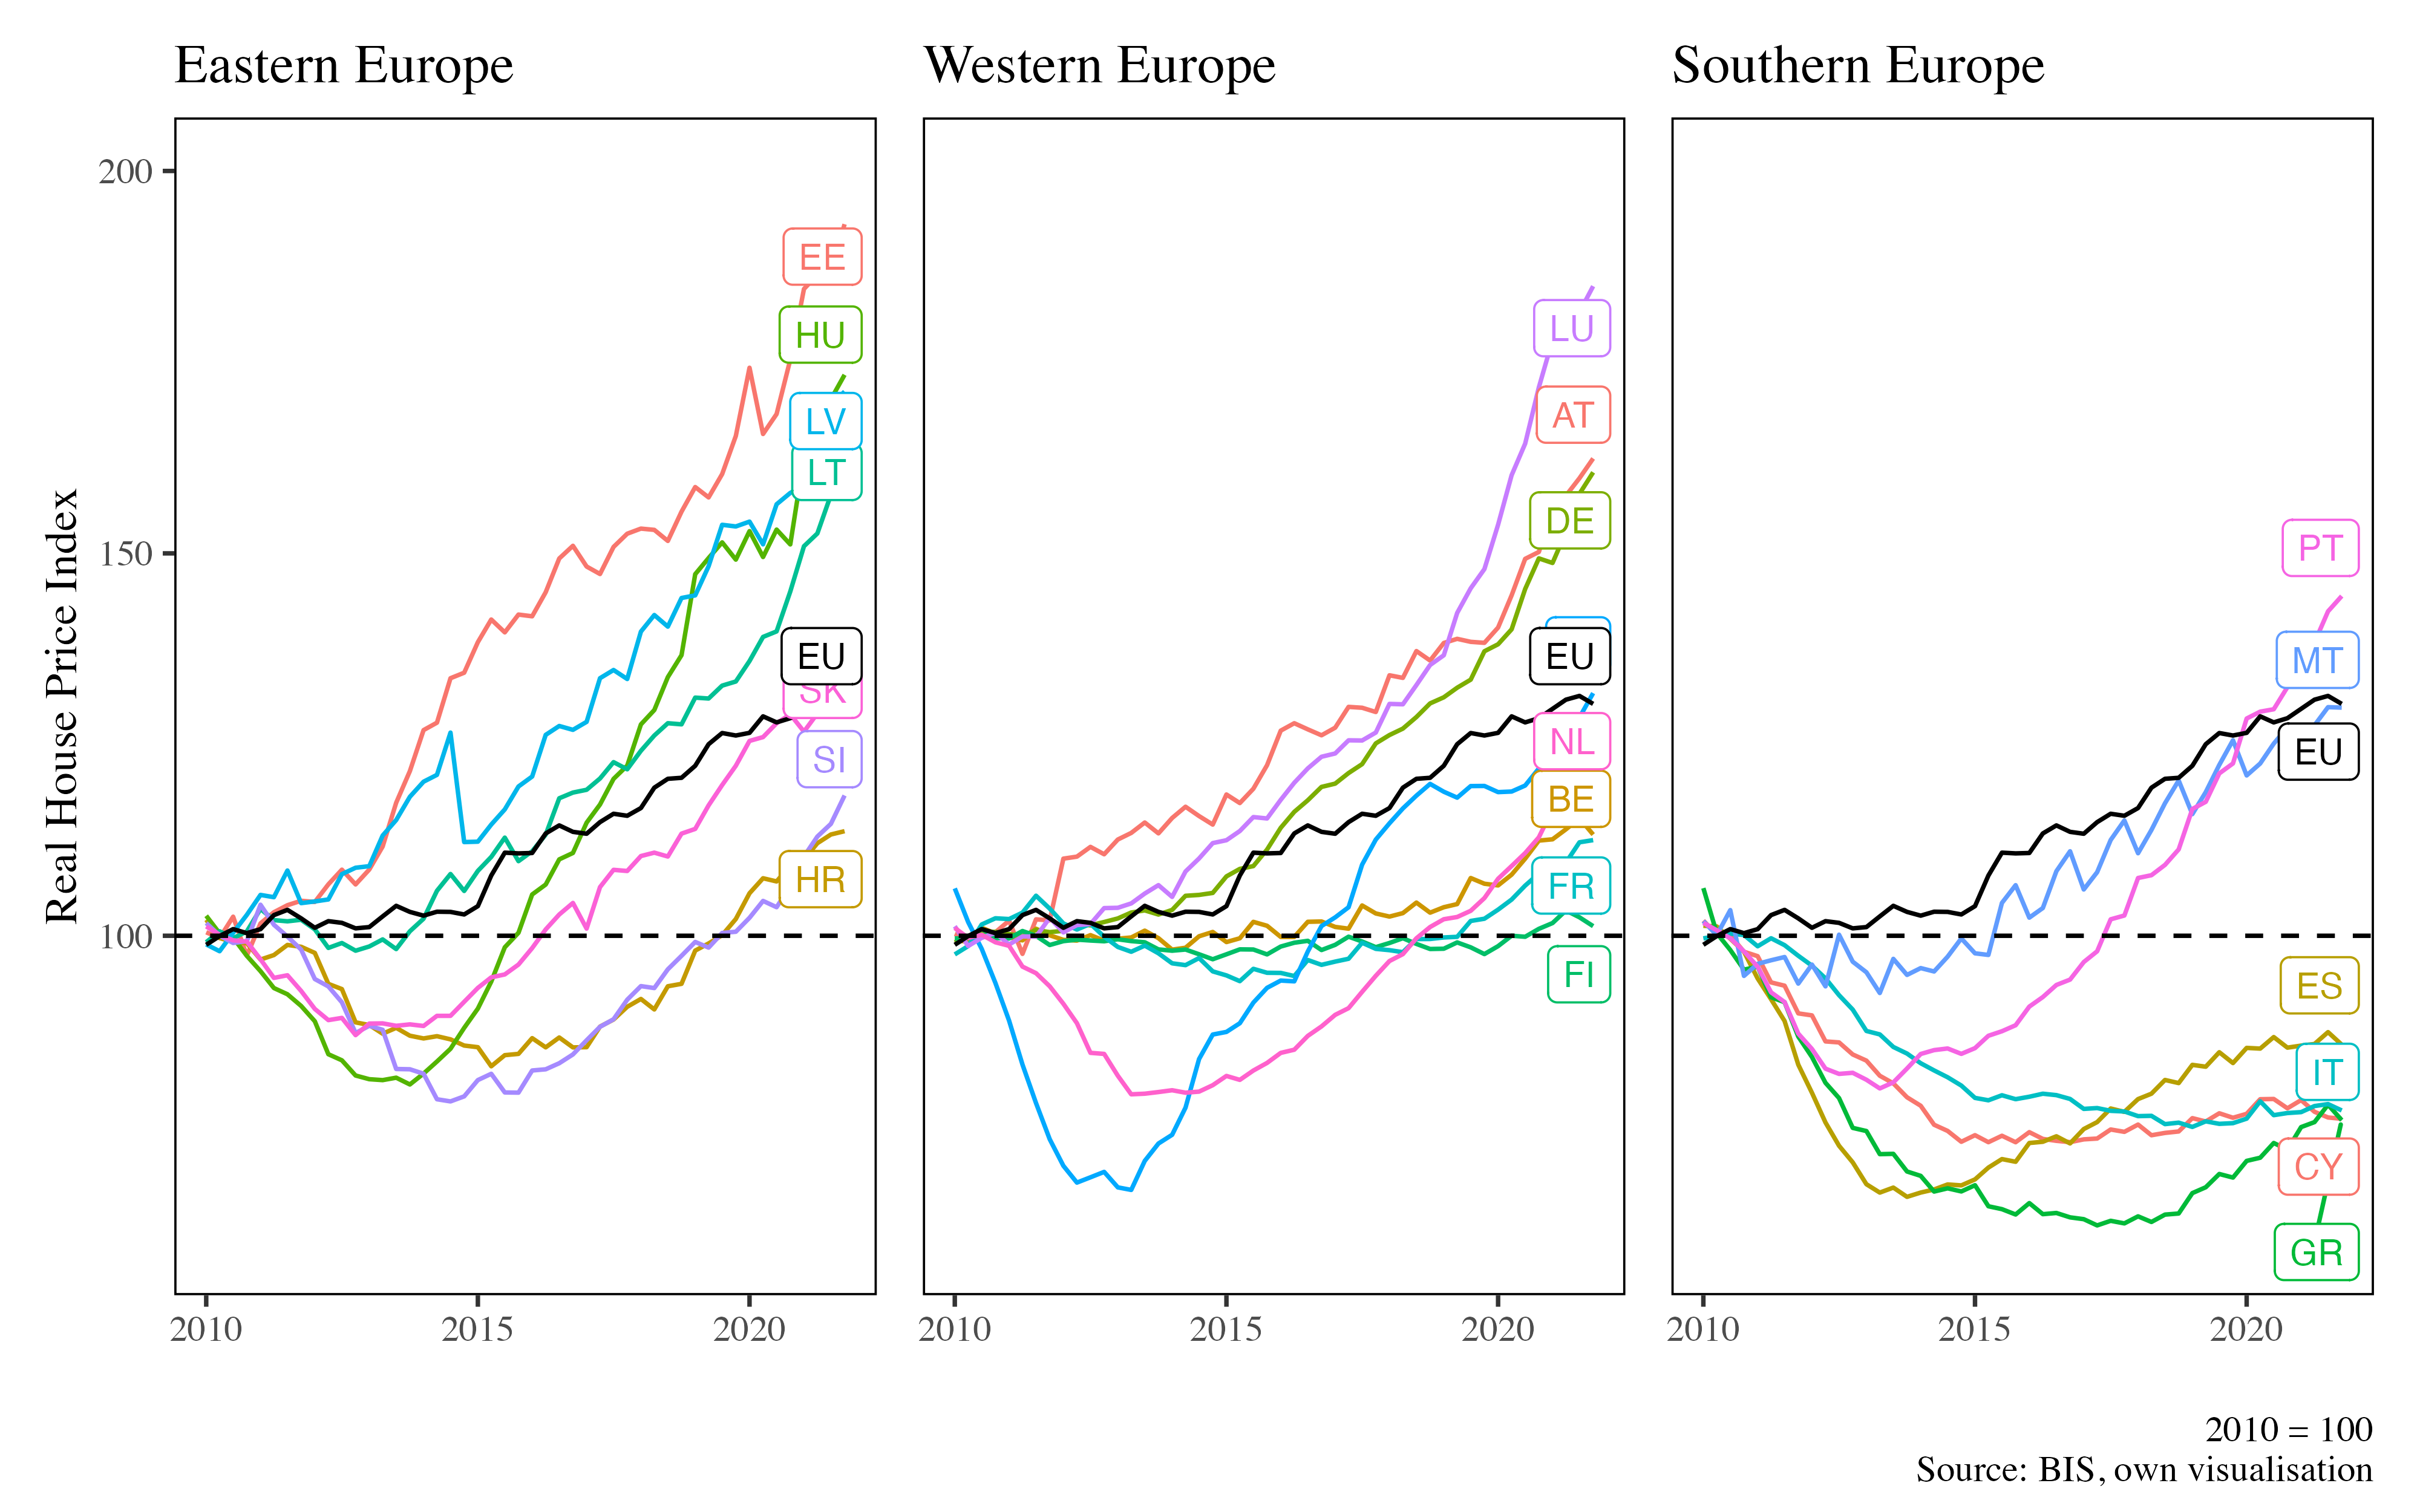
\includegraphics[keepaspectratio]{../output/desc/house_prices_europe.png}}

}

\caption{\label{fig-prices}Residential Property Price Index}

\end{figure}%

For Housing Price Data, the Residential Property Price Dataset from the
Bank of International Settlement (BIS) is used
(\citeproc{ref-scatignaResidentialPropertyPrice2014}{Scatigna, Szemere,
and Tsatsaronis 2014}). The dataset is widely used in cross country
comparisons (i.e.
\citeproc{ref-runstlerBusinessHousingCredit2018}{Rünstler and Vlekke
2018}) and includes quarterly time series for most developed countries
in real terms.

Housing Prices in the Eurozone plateaud until 2015 and experienced a
strong increase afterwards, as visible in Figure~\ref{fig-prices}. This
average marks strong differences in the individual member states.
Southern European Countries like Spain, Italy and Greece experienced a
devaluation after 2010, while many western and eastern european
countries show strong increases in property price indices. Price Indices
in Estonia and Luxemburg almost doubled in the observed timeframe, while
they declined by 25 index points in Greece.

Stock prices are represented using the Euro Stoxx 50 index, which
includes 50 large firms from 11 Eurozone countries, offering broad
representation of the region's equity markets. The index captures
approximately 60\% of total market capitalization and serves as a
standard benchmark for European stock market performance (e.g
\citeproc{ref-brechmannRiskManagementHighdimensional2013}{Brechmann and
Czado 2013}).

The final panel dataset includes asset holdings for the three wealth
groups in 21 countries as well as the Eurozone as an aggregate, measured
in nominal values. The number of observations per country ranges from 17
in Latvia to 49 in Greece, totaling 860 observations. This is
complemented by housing price indices for all countries over the
observed time frames and the European stock price index for the entire
time period.

After presenting the data sources used in the analysis, the next section
provides some stylized facts and descriptive statistics drawn from the
DWA.

\section{Stylized Facts about the Wealth
Distribution}\label{sec-descriptive}

The portfolios of the bottom 50\% display the largest heterogeneities
across Europe\footnote{The complete breakdown for all european countries
  is provided in Figure~\ref{fig-portfolio-indiv} in Appendix C.}. In
most countries, they closely resemble the composition of the middle
class with housing as the main asset (examples include Italy, Ireland
and Finland). Outliers to this rule include Germany, Austria and the
Netherlands. The wealth of the lower half in these countries is
predominantly made up of the other assets and housing contributes less
than 50\% to total wealth.

The distribution of these asset classes among the wealth groups in the
Eurozone is described in Figure~\ref{fig-distribution}. As visible,
Housing is distributed most equally of the wealth categories, with the
Top Decile owning 47\% of the total Housing Wealth. It is followed by
Net Wealth with 57\%, and Financial Wealth and Business Wealth with 72\%
and 85\% respectively.

This sequence holds in all european countries, with the absolute numbers
differing considerably\footnote{The expanded version of
  Figure~\ref{fig-distribution} with country-specific distributions is
  available as Figure~\ref{fig-distribution-indiv} in Appendix C}. While
almost all financial wealth is owned by the top decile in Croatia and
Greece, it is less than half in the Netherlands and Malta. For business
wealth, the most significant share held by the top 10\% is in Austria
and Germany, while Greece and Cyprus feature the most equal
distribution. In Housing Wealth, it is not the share of the top 10\%
that varies much, but the bottom 50\%. In Germany, Austria and the
Netherlands they possess below 2\% of the asset, while their
counterparts in Slovakia and Lithuania own more than 15\%.

\begin{figure}

\begin{minipage}{0.50\linewidth}

\begin{figure}[H]

\centering{

\pandocbounded{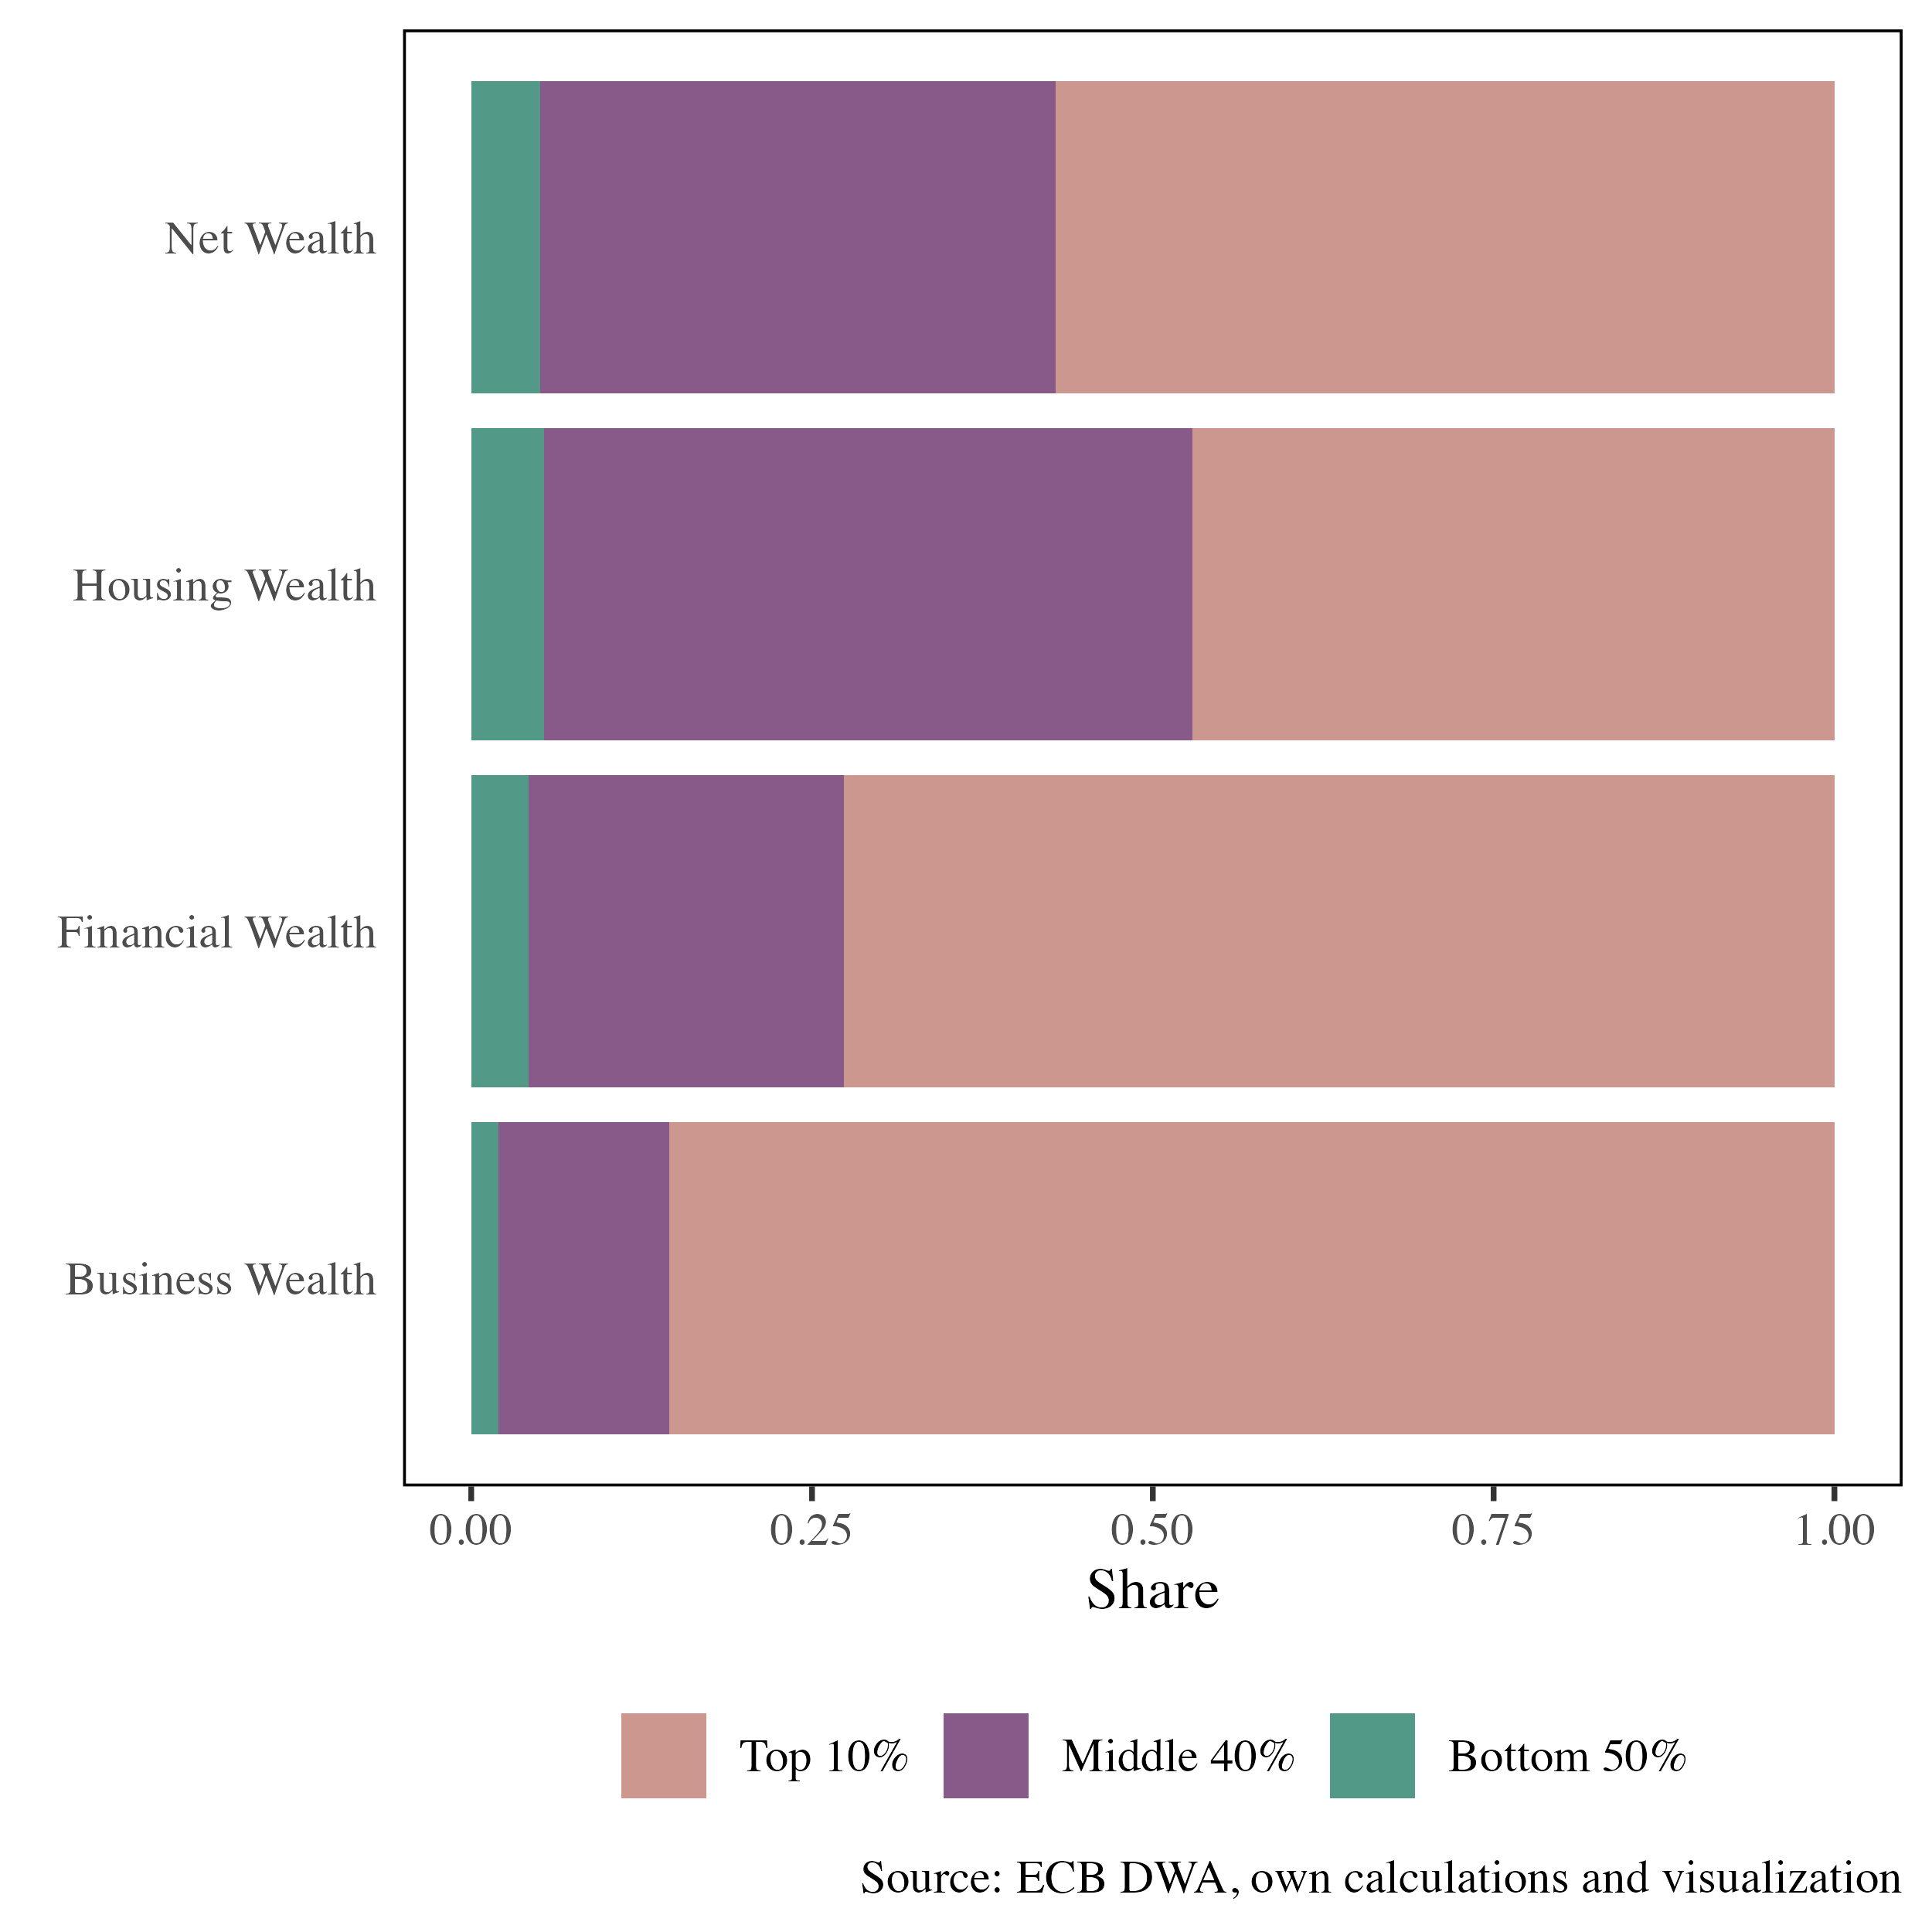
\includegraphics[keepaspectratio]{../output/desc/asset_distribution_decile.png}}

}

\caption{\label{fig-distribution}Asset distribution among wealth groups
(Eurozone Average)}

\end{figure}%

\end{minipage}%
%
\begin{minipage}{0.50\linewidth}

\begin{figure}[H]

\centering{

\pandocbounded{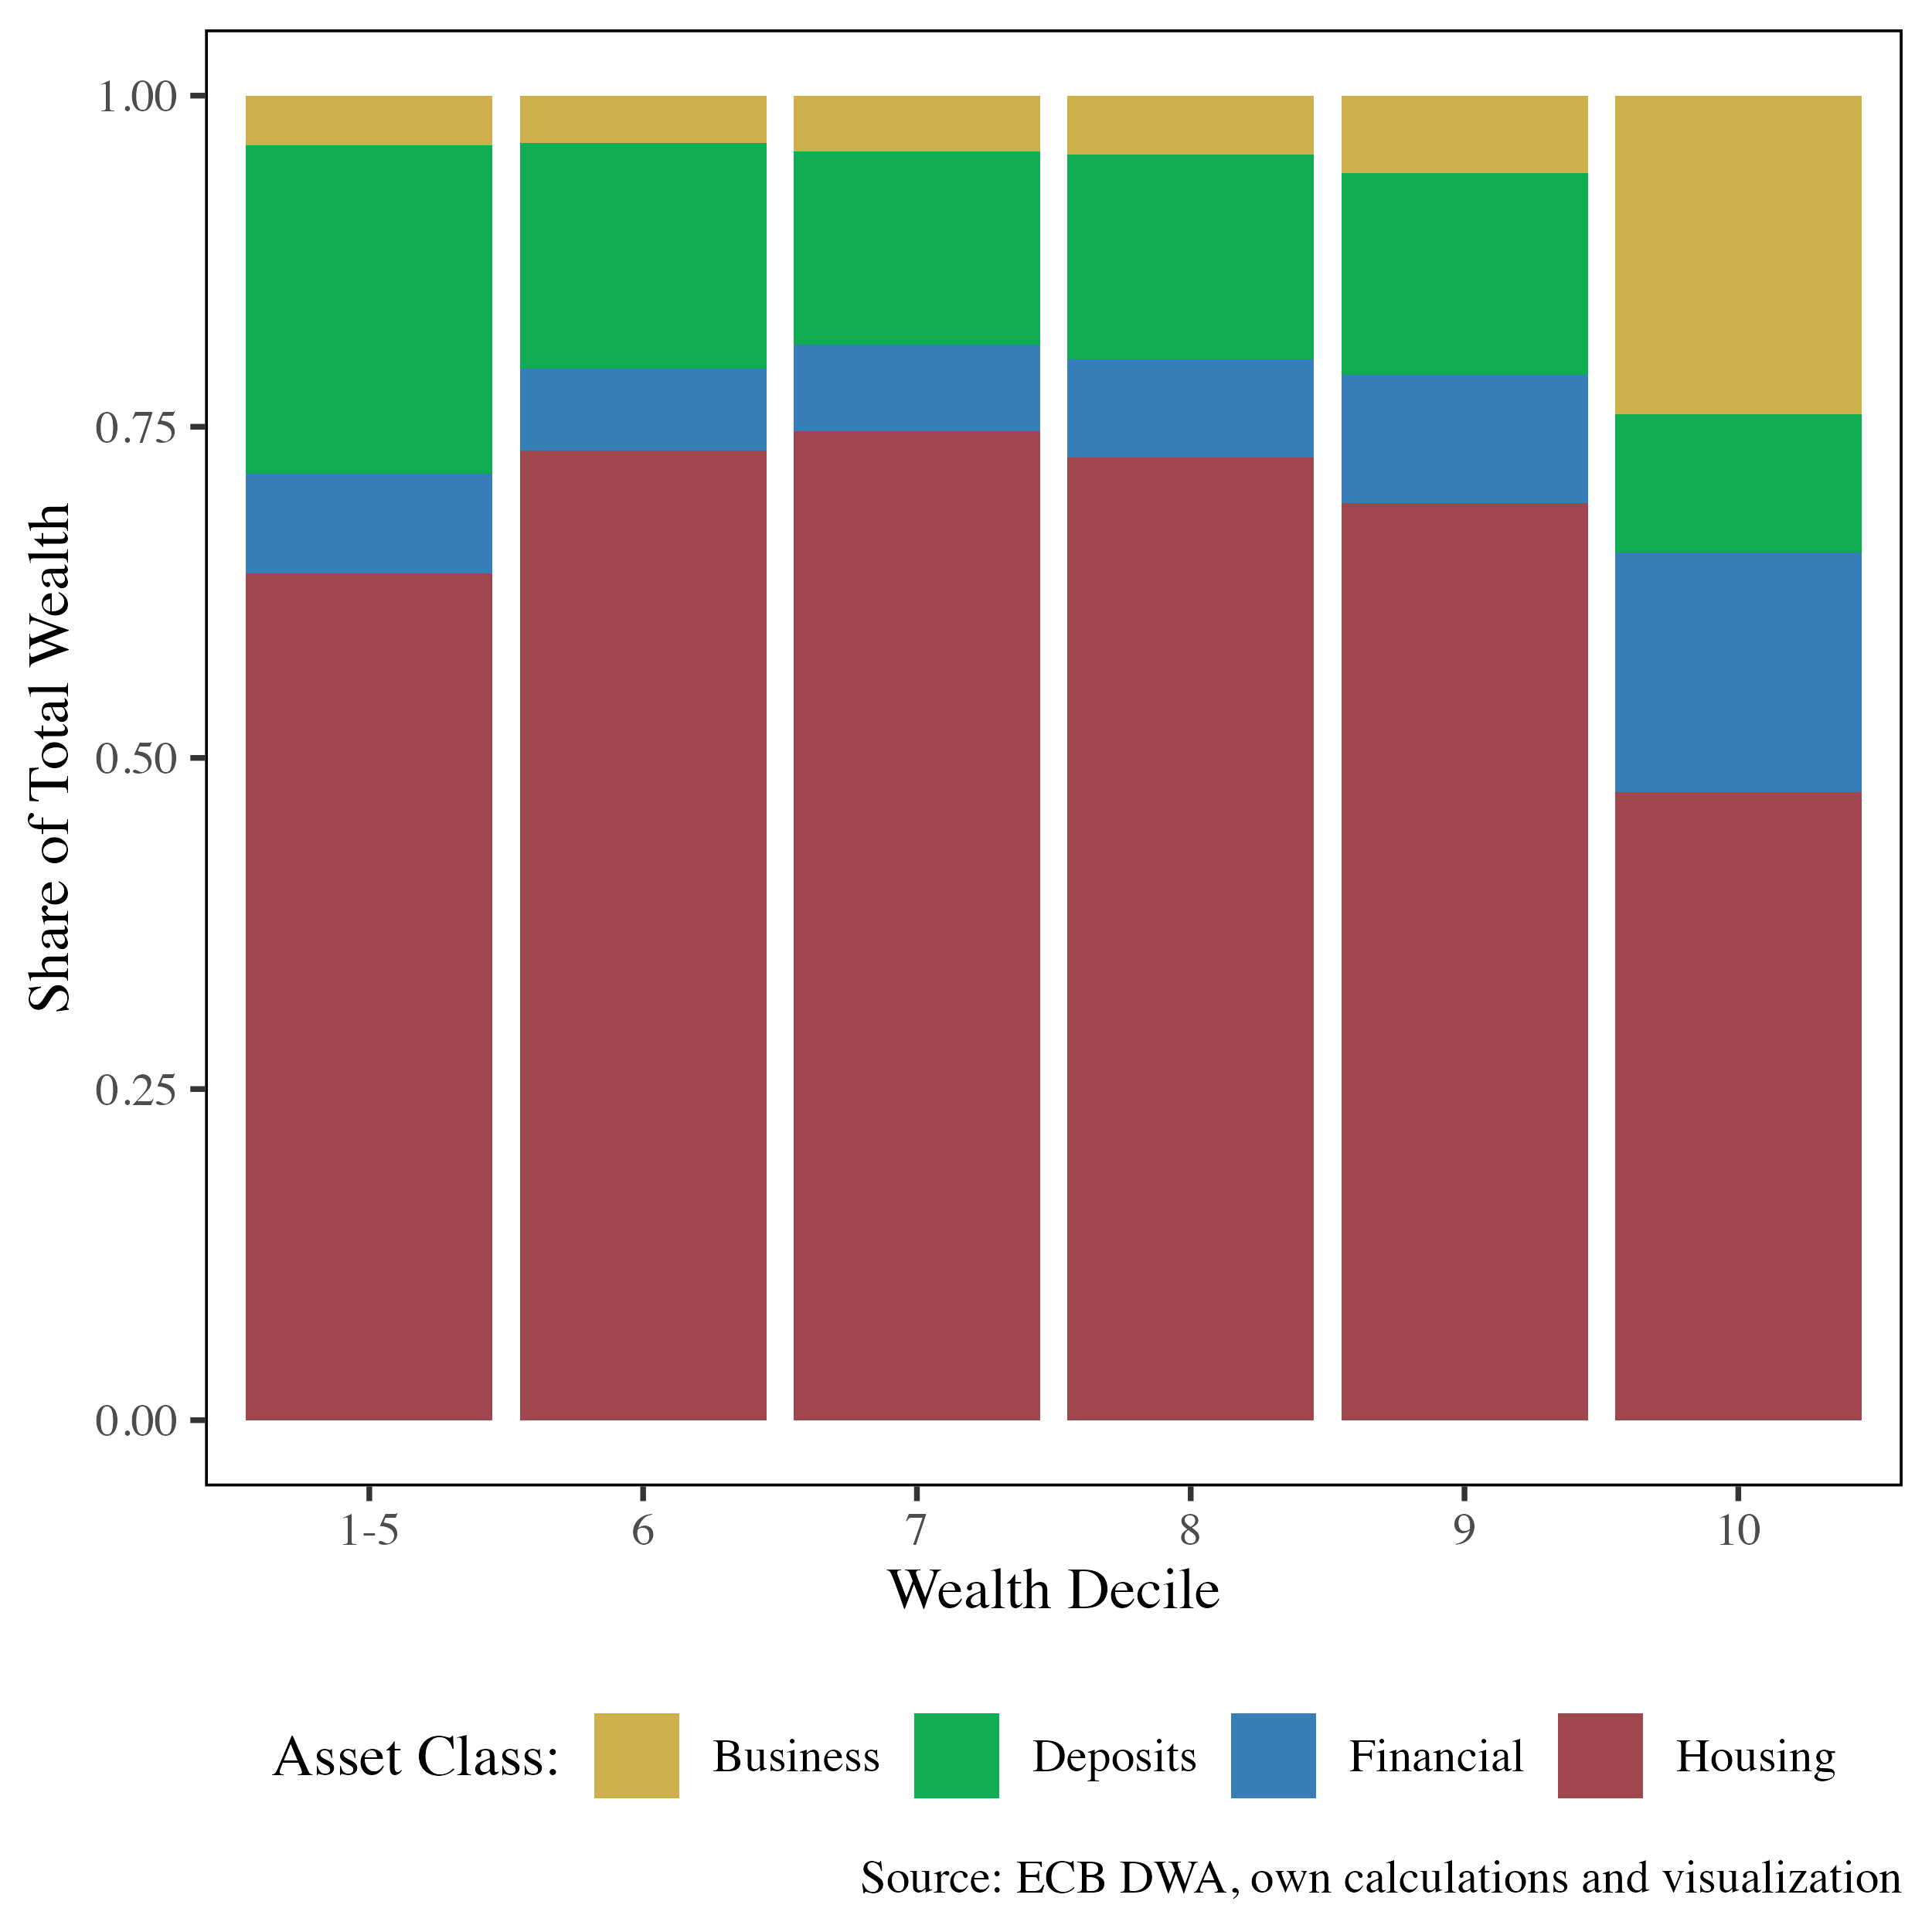
\includegraphics[keepaspectratio]{../output/desc/portfolio_europe.png}}

}

\caption{\label{fig-portfolio}Portfolio Composition of Deciles (Eurozone
Average)}

\end{figure}%

\end{minipage}%

\end{figure}%

Figure~\ref{fig-trends} tracks the portfolios of the wealth groups over
the observed time frame. The figure confirms the large heterogeneity of
wealth portfolios in the literature and additionally adds a time
dimension displaying the diffferent growth trends of net wealth.

The lower half of the distribution have little wealth, with housing and
deposits playing the largest role. They are highly leveraged and
essentially did not increase their net wealth until 2015, after which it
grew slowest of all groups. The portfolio of the Middle 40\% is
dominated by housing. Compared to the Bottom 50\%, they exhibit much
higher net wealth and much lower debt. In the top decile, Business as
well as Financial Wealth play a larger role, while debt plays a smaller
one. The net wealth of the top 10\% grew fastest, from 539 thousand
euros to 849 thousand euros per capita, a 57\% increase in the span of
12 years.

\begin{figure}[h]

\centering{

\pandocbounded{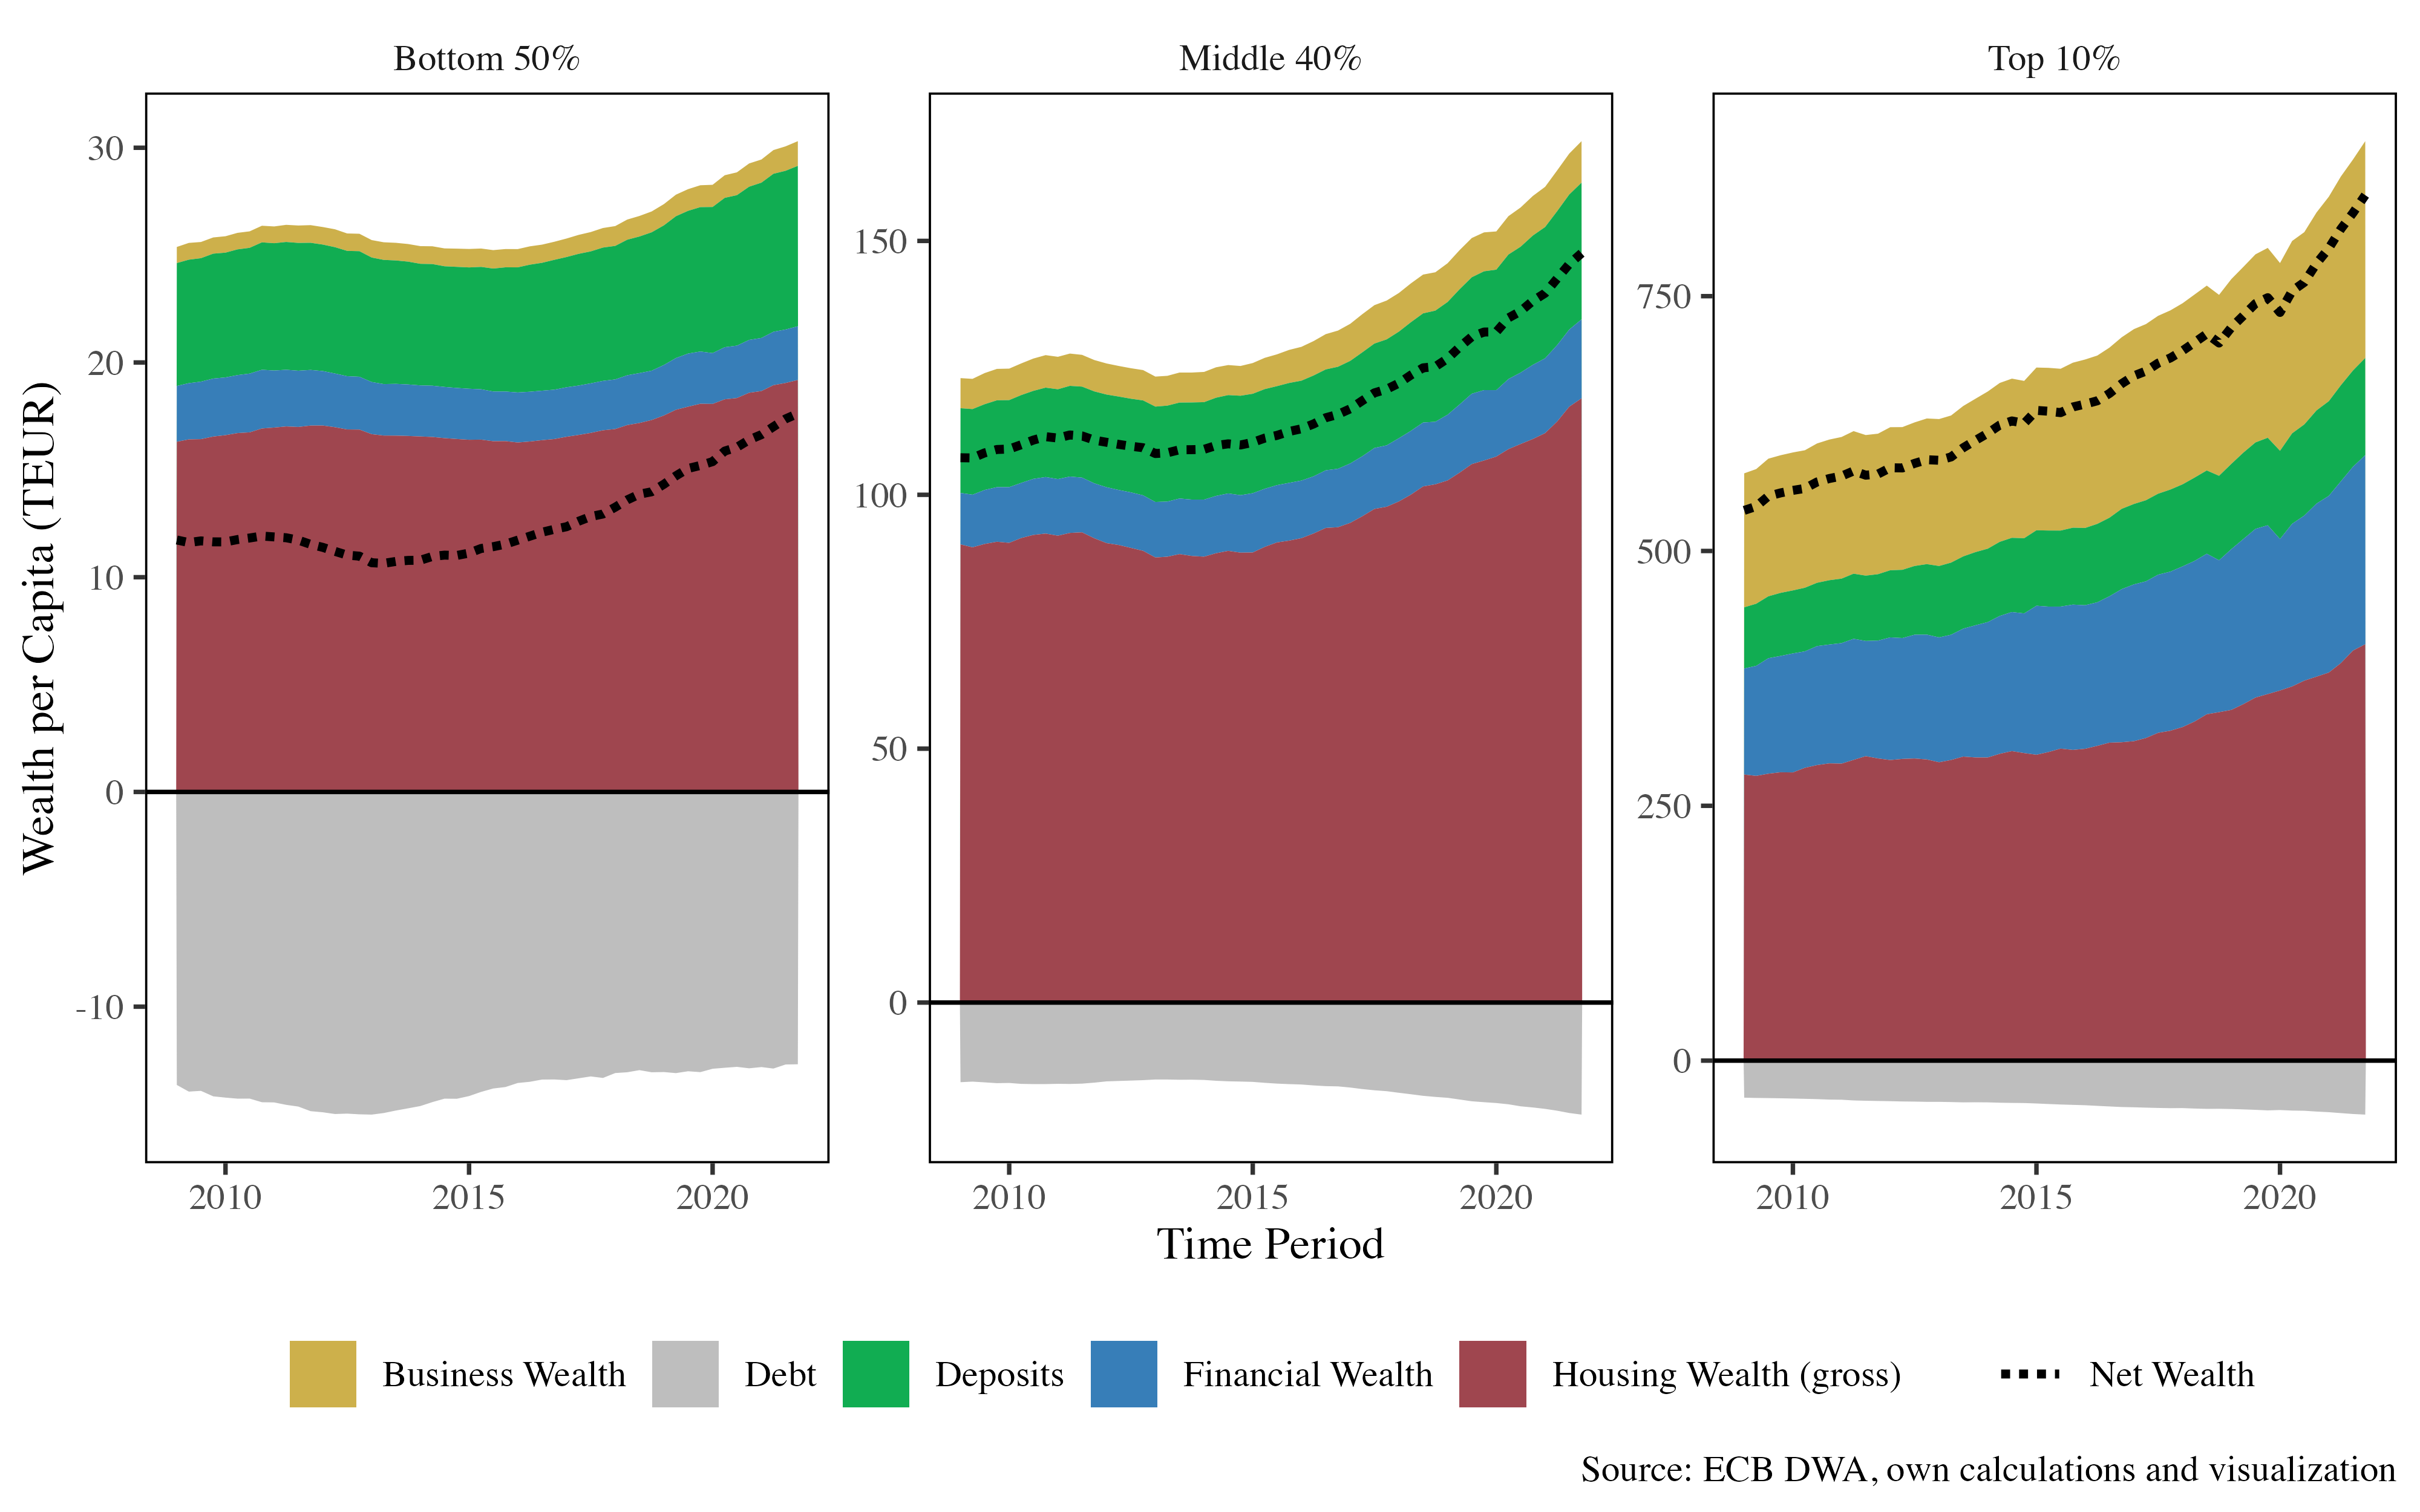
\includegraphics[keepaspectratio]{../output/desc/asset_distribution_over_time.png}}

}

\caption{\label{fig-trends}Differential Wealth Trends (Eurozone
Average)}

\end{figure}%

These differences in portfolio size and composition suggest that changes
in asset prices are likely to affect each segment of the distribution in
distinct ways. The next section sets out the econometric framework used
to quantify these effects.

\section{Empirical Strategy}\label{sec-strategy}

As described above, different segments of the wealth distribution hold
different portfolios, in size as well as in composition of asset
classes. Their net wealth therefore reacts in distinct ways to identical
changes in valuation of assets. This has a direct effect on the share of
overall wealth held by the segment and consequently on general wealth
inequality.

To estimate this response, a panel regression outlined in
Equation~\ref{eq-regression} is estimated:

\begin{equation}\phantomsection\label{eq-regression}{
\Delta \log (\omega_{i,t}^g) = \beta_0 + \beta_h \Delta \log (p_{i,t}^h) + \beta_s \Delta \log(p^s_{t})+ \epsilon_t
}\end{equation}

\(\Delta \log\) is the first difference of the log, as in
\(\Delta \log (x_t) = \log(x_t) - \log(x_{t-1})\). \(\omega_{i,t}^g\) is
the wealth share of a wealth group \(g\) (Bottom 50\%, Middle 40\%, Top
10\%) in country \(i\) in quarter \(t\). \(p^h\) describes the housing
price index and \(p^s\) the stock market index. \(\epsilon_t\) is an
error term. The resulting estimates can be interpreted as the elasticity
of the groups wealth share with respect to asset prices
(\citeproc{ref-wooldridgeIntroductoryEconometricsModern2013}{Wooldridge
2013, 44}).

Some regressions are extended to include country and time fixed effects.
To control for seasonal patterns and macroeconomic shocks, one
specification also includes separate fixed effects for each quarter and
each year. Quarter fixed effects are defined as categorical indicators
for Q1 to Q4, while year fixed effects cover the years 2011 to 2022,
capturing annual shocks common across countries.

A potential concern with this type of panel structure is spatial
dependence. As the cross-section of countries is not randomly sampled,
they are subject to common unobserved and observed disturbances, which
potentially bias the standard errors of the parameter estimations. To
adress this issue, the standard errors are computed using the spatial
correlation consistent (SCC) method by Driscoll and Kraay
(\citeproc{ref-driscollConsistentCovarianceMatrix1998}{1998}).

Another problem is the heterogeneity in responses subsumed under the
parameter estimates in an Ordinary Least Squares (OLS) Regression. Due
to differing portfolio compositions of the same wealth groups across
Europe, \(\beta_h\) and \(\beta_s\) will not have the same slope in all
countries and their estimates will not be able to explain the large
variation.

To adress this, the estimates are additionally calculated with the mean
group estimator (MGE) proposed by Pesaran and Smith
(\citeproc{ref-pesaranEstimatingLongrunRelationships1995}{1995}). This
estimator allows for heterogeneity in individual coefficients and error
terms by running separate regressions for each unit. Resulting estimates
are averaged as \(\hat{\beta}^{MG} = 1/N \sum_{i=1}^N \hat{\beta}_i\)
(\citeproc{ref-milloPanelTimeSeries2018}{Millo and Croissant 2018,
190}).

The MGE requires that \(T \ge p\) and \(N\) and \(T\) are sufficiently
large. Using Monte Carlo simulations, Hsiao, Pesaran, and Tahmiscioglu
(\citeproc{ref-hsiaoBayesEstimationShortrun1999}{1999}) find that
\(T=5\) leads to considerable estimation error, while \(T=20\) yields
reliable results. The DWA dataset places well within the recommended
range for applying the MGE, with \(N=21\) and \(T\) ranging from 17 to
49 across countries

One specification of the MGE is demeaned cross-sectionally, which
reduces the influence of common factors. It is comparable to Time Fixed
Effects in an OLS estimate
(\citeproc{ref-coakleyUnobservedHeterogeneityPanel2006}{Coakley,
Fuertes, and Smith 2006}). Both the standard as well as the demeaned MGE
use the implementation in R by Croissant et al.
(\citeproc{ref-croissantPlmLinearModels2023}{2023}).

Additionally, regressions are estimated separately for each country.
This allows for the interpretation of country-specific responses to
identical price movements and helps identify outliers. One problem with
the OLS estimator in real world time series data like the one used in
this analysis is standard errors are autocorrelated. This could result
in biased estimates of the standard errors, as one of the core
assumptions of the OLS estimator is not fulfilled. To address the
autocorrelation and potential heteroskedasticity in the time series,
standard errors are computed using the Newey-West estimator
(\citeproc{ref-neweyHypothesisTestingEfficient1987}{Newey and West
1987}). This method corrects the standard errors by computing a
heteroskedasticity and autocorrelation consistent variance matrix with a
lag window to capture common disturbances
(\citeproc{ref-pesaranTimeSeriesPanel2015}{Pesaran 2015, 113}).

The following section applies this framework to estimate the
relationship between asset price changes and wealth shares.

\section{Wealth Share Elasticities: Panel Regression}\label{sec-panel}

\begin{table}

\caption{\label{tbl-panelT10}Top 10\% Panel Regression}

\centering{

\fontsize{9.0pt}{10.8pt}\selectfont
\begin{tabular*}{\linewidth}{@{\extracolsep{\fill}}lccccc}
\toprule
 & \multicolumn{3}{c}{OLS Estimator} & \multicolumn{2}{c}{Mean Group Estimator} \\ 
\cmidrule(lr){2-4} \cmidrule(lr){5-6}
  & (1) & (2) & (3) & (4) & (5) \\ 
\midrule\addlinespace[2.5pt]
House Prices & -0.091*** & -0.077*** & -0.056 & -0.055*** & -0.057*** \\ 
 & (0.013) & (0.009) & (0.047) & (0.020) & (0.018) \\ 
Stock Prices &  & 0.017*** & 0.027*** &  & 0.014*** \\ 
{} & {} & {(0.007)} & {(0.009)} & {} & {(0.004)} \\ 
\midrule
Unit Fixed Effects & No & Yes & Yes & - & - \\ 
Time Fixed Effects & Yes & No & Year + Quarter & Yes & No \\ 
\midrule
{N} & {860} & {860} & {860} & {860} & {860} \\ 
R² & 0.071 & 0.087 & 0.076 & 0.443 & 0.313 \\ 
Adj. R² & 0.013 & 0.062 & 0.050 & 0.408 & 0.269 \\ 
\bottomrule
\end{tabular*}
\begin{minipage}{\linewidth}
* p < 0.1, ** p < 0.05, *** p < 0.01\\
OLS Estimators use the SCC Standard Errors by Millo (2017)\\
\end{minipage}

}

\end{table}%

Table~\ref{tbl-panelT10} reports the results of the panel regression for
the share of the Top 10\%. The first column includes time fixed effects,
which absorb the stock prices due to the identical nature of the index
in every country. Column 2 drops the time fixed effects, and includes
unit fixed effects, while the third specification adds year and quarter
fixed effects to control for seasonality. Column 4 presents calculations
using the Demeaned MGE, which again absorb the estimates for stock
prices. Column 5 uses the standard MGE. A separate regression with year
and quarter fixed effects is not included, as it is identical. Including
lags of the dependent variable does not materially alter the estimated
effects. Full results with lags are reported in Table~\ref{tbl-dynamic}
in Appendix E.

The top 10\% wealth share decreases in response to house price
increases. The estimates are consistently negative in all specifications
and statistically significant, ranging from -0.091 in the first column
to -0.057 in the last and preferred specification. A 10\% increase in
House Prices leads to approximately a half percentage point decrease in
the top decile wealth share.

Rising stock prices are found to have an effect in the opposite
direction. Estimates for the elasticity of the top decile wealth share
range from 0.027 in the third specification and 0.014 in the last. An
increase in stock prices increase the share of wealth hold by the Top
10\%, while an increase in house prices compresses the share.

The OLS estimates for this as well as the other segments of the wealth
distribution display a low coefficient of determination due to the
heterogeneity in the data. Using the Mean Group Estimator, the models
can explain above 20\% of the variance in the standard configuration and
above 30\% in the demeaned configuration for all groups.

\begin{table}

\caption{\label{tbl-panelM40}Middle 40\% Panel Regression}

\centering{

\fontsize{9.0pt}{10.8pt}\selectfont
\begin{tabular*}{\linewidth}{@{\extracolsep{\fill}}lccccc}
\toprule
 & \multicolumn{3}{c}{OLS Estimator} & \multicolumn{2}{c}{Mean Group Estimator} \\ 
\cmidrule(lr){2-4} \cmidrule(lr){5-6}
  & (1) & (2) & (3) & (4) & (5) \\ 
\midrule\addlinespace[2.5pt]
House Prices & 0.058*** & 0.036*** & -0.010 & 0.033** & 0.031* \\ 
 & (0.012) & (0.009) & (0.040) & (0.015) & (0.016) \\ 
Stock Prices &  & -0.019** & -0.031*** &  & -0.014*** \\ 
{} & {} & {(0.008)} & {(0.009)} & {} & {(0.005)} \\ 
\midrule
Unit Fixed Effects & No & Yes & Yes & - & - \\ 
Time Fixed Effects & Yes & No & Year + Quarter & Yes & No \\ 
\midrule
{N} & {860} & {860} & {860} & {860} & {860} \\ 
R² & 0.027 & 0.049 & 0.034 & 0.388 & 0.258 \\ 
Adj. R² & -0.034 & 0.023 & 0.008 & 0.349 & 0.210 \\ 
\bottomrule
\end{tabular*}
\begin{minipage}{\linewidth}
* p < 0.1, ** p < 0.05, *** p < 0.01\\
OLS Estimators use the SCC Standard Errors by Millo (2017)\\
\end{minipage}

}

\end{table}%

Contrasting effects to those of the top decile are identified for the
Middle 40\% (Table~\ref{tbl-panelM40}). The elasticity of their wealth
share with respect to house prices is positive, ranging from 0.058 in
Model (1) to 0.031 in the preferred Model (5). An outlier is the
estimate for the specification with Year and Quarter Fixed Effects,
which is however not statistically significant. Stock prices on the
other hand have a statistically significant negative effect on the
middle segment of the wealth distribution. A 10\% increase in stock
prices leads to a decline in the share of net wealth of approximately
0.14 to 0.31 percentage points, depending on the specification.

The Bottom half of the wealth distribution responds similarly to the
middle 40\% in direction, albeit with greater magnitude. Estimates for
the House Price elasticity range from 0.189 to 0.481. Conversely,
accelerating stock prices by 10\% decreases the share of the group by
0.28 percentage points to 0.51 percentage points.

This group is notable for its lack of statistical significance for most
coefficient values, particularly in specifications that use the mean
group estimator. As outlined above, it is the lower half that exhibits
the most variation in their wealth portfolio and positions. Therefore,
they will display the most variation in their response to price
movements of their assets, which cannot be averaged without high
standard errors.

\begin{table}

\caption{\label{tbl-panelB50}Bottom 50\% Panel Regression}

\centering{

\fontsize{9.0pt}{10.8pt}\selectfont
\begin{tabular*}{\linewidth}{@{\extracolsep{\fill}}lccccc}
\toprule
 & \multicolumn{3}{c}{OLS Estimator} & \multicolumn{2}{c}{Mean Group Estimator} \\ 
\cmidrule(lr){2-4} \cmidrule(lr){5-6}
  & (1) & (2) & (3) & (4) & (5) \\ 
\midrule\addlinespace[2.5pt]
House Prices & 0.481*** & 0.393*** & 0.189 & 0.212 & 0.253 \\ 
 & (0.109) & (0.062) & (0.175) & (0.192) & (0.179) \\ 
Stock Prices &  & -0.028* & -0.051 &  & -0.029 \\ 
{} & {} & {(0.016)} & {(0.033)} & {} & {(0.022)} \\ 
\midrule
Unit Fixed Effects & No & Yes & Yes & - & - \\ 
Time Fixed Effects & Yes & No & Year + Quarter & Yes & No \\ 
\midrule
{N} & {860} & {860} & {860} & {860} & {860} \\ 
R² & 0.065 & 0.056 & 0.043 & 0.361 & 0.340 \\ 
Adj. R² & 0.006 & 0.030 & 0.016 & 0.320 & 0.298 \\ 
\bottomrule
\end{tabular*}
\begin{minipage}{\linewidth}
* p < 0.1, ** p < 0.05, *** p < 0.01\\
OLS Estimators use the SCC Standard Errors by Millo (2017)\\
\end{minipage}

}

\end{table}%

\section{Country-Level Variation}\label{sec-indiv}

To examine these heterogeneous effects across countries, the regression
is re-estimated separately for each country following
Equation~\ref{eq-indiv}\footnote{Full regression tables are presented in
  Appendix D}. As mentioned above, the standard errors are
heteroskedasticity and autocorrelation consistent by use of the method
of Newey and West
(\citeproc{ref-neweyHypothesisTestingEfficient1987}{1987}).

\begin{equation}\phantomsection\label{eq-indiv}{
\Delta \log (\omega_{t}^g) = \beta_0 + \beta_h \Delta \log (p_{t}^h) + \beta_s \Delta \log(p^s_{t})+ \epsilon_t
}\end{equation}

Figure Figure~\ref{fig-coeffplot} displays the resulting country-level
coefficients for housing prices for each segment of the wealth
distribution. Estimates are ordered by magnitude and colored by
statistical significance, with their standard errors represented by the
error bars\footnote{A corresponding stock price coefficient plot is
  available in Appendix F.}.

Visible in the panels is the large heterogeneity in all wealth segments.
Estimates for the top decile range from -0.20 for Spain to 0.19 for the
Netherlands. The majority of the coefficients with statistical
significance are negative, which confirms the results from
Table~\ref{tbl-panelT10}. For the middle 40\%, the coefficients fall
between -0.11 in the Netherlands and 0.13 in France, with a large share
of countries for which the null hypothesis cannot be rejected. Results
in the lower half of the wealth distribution exceed those of the other
groups. The Netherlands has an estimated elasticity of -2.71, which
indicates that a 1\% increase in house prices decreases the share of net
wealth held by that group by 2.7\%. In contrast, they increase their
share by 2.18\% in Ireland in response to an identical increase in house
prices.

Boelhouwer (\citeproc{ref-boelhouwerHousingMarketNetherlands2020}{2020})
present explanations for the dutch outlier results. The social housing
sector in the Netherlands is larger than in other european countries,
promising affordable renting for poorer households. Additionally, new
stricter mortgage lending requirements were implemented in 2011,
reducing the ability of first time buyers to afford sufficient housing.
This could explain the very low share of housing wealth owned by the
bottom 50\% documented in Figure~\ref{fig-distribution-indiv} and the
negative effect in response to increasing house prices.

\begin{figure}[h]

\centering{

\pandocbounded{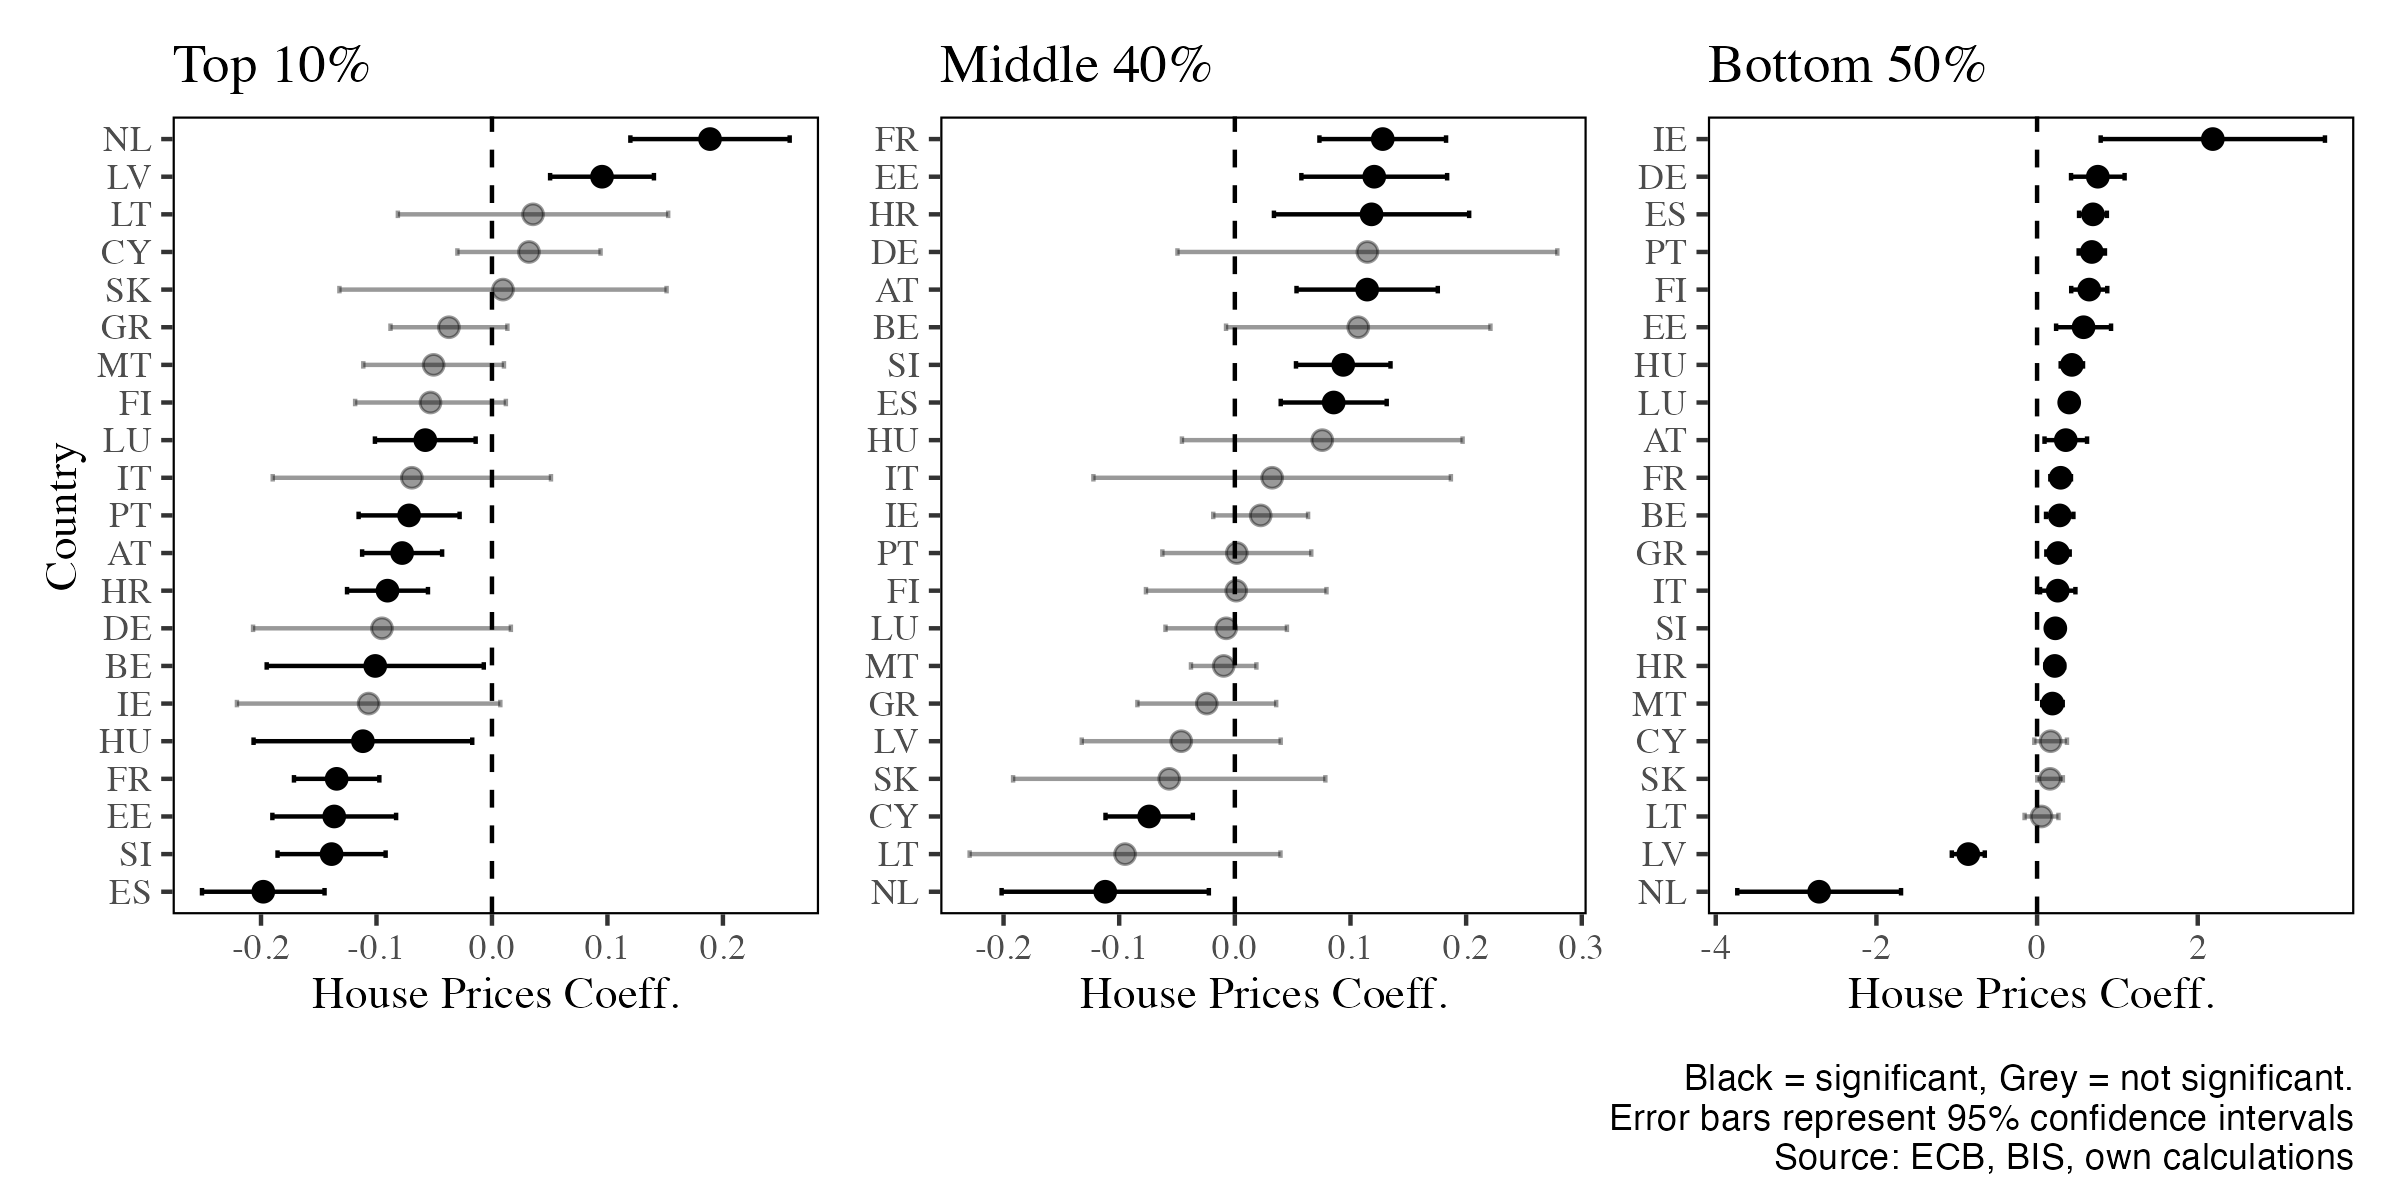
\includegraphics[keepaspectratio]{../output/ts_tables/HP_coeff.png}}

}

\caption{\label{fig-coeffplot}House Price Coefficient Plots}

\end{figure}%

In general, the individual regressions support the panel model results.
Accelerating stock prices profits the upper decile of the wealth
distribution, at the expense of the rest of the population. House prices
have a contrary effect, increasing the share of the bottom 50\% and
middle 40\%. Statistical significance as well as \(R^2\) varies due to
heterogeneity in the responses in european countries.

To address the outlier effect of the Netherlands, the panel regressions
are re-estimated excluding this country. Table Table~\ref{tbl-panelNL}
compares the results of the preferred specification using the standard
mean group estimator with and without the Dutch data.

Excluding the Netherlands slightly reduces the magnitude of the
coefficients for housing prices on the Top 10\% and Middle 40\%, but the
signs and significance remain stable. For the Top 10\%, the negative
effect of house prices weakens from -0.057 to -0.069, while for the
Middle 40\%, the positive effect increases slightly and becomes more
statistically significant.

The most notable change is for the bottom 50\%. The coefficient on house
prices increases from 0.253 to 0.395 and becomes statistically
significant at the 1\% level. This suggests that, once the outlier is
removed, the effect of housing prices on the lower half of the
distribution becomes clearer and more robust.

Stock price effects remain broadly stable across all specifications,
with a significant positive effect on the Top 10\% and a negative effect
on the Middle 40\%, consistent with prior estimates. No meaningful
change is observed when the Netherlands is excluded

Overall, the results strengthen the interpretation that rising house
prices tend to benefit the Bottom 50\% and Middle 40\%, while rising
stock prices disproportionately benefit the Top 10\%. Having established
the sensitivity of wealth segments to asset prices, the next section
simulates the evolution of wealth shares under different scenarios.

\begin{table}

\caption{\label{tbl-panelNL}Panel Regression without the Netherlands}

\centering{

\fontsize{9.0pt}{10.8pt}\selectfont
\begin{tabular*}{\linewidth}{@{\extracolsep{\fill}}lcccccc}
\toprule
 & \multicolumn{2}{c}{Top 10\%} & \multicolumn{2}{c}{Middle 40\%} & \multicolumn{2}{c}{Bottom 50\%} \\ 
\cmidrule(lr){2-3} \cmidrule(lr){4-5} \cmidrule(lr){6-7}
  & (1) & (2) & (3) & (4) & (5) & (6) \\ 
\midrule\addlinespace[2.5pt]
House Prices & -0.057*** & -0.069*** & 0.031* & 0.037** & 0.253 & 0.395*** \\ 
 & (0.018) & (0.015) & (0.016) & (0.016) & (0.179) & (0.115) \\ 
Stock Prices & 0.014*** & 0.012*** & -0.014*** & -0.014*** & -0.029 & -0.008 \\ 
{} & {(0.004)} & {(0.004)} & {(0.005)} & {(0.005)} & {(0.022)} & {(0.007)} \\ 
\midrule
NL included & Yes & No & Yes & No & Yes & No \\ 
\midrule
{N} & {860} & {832} & {860} & {832} & {860} & {832} \\ 
R² & 0.313 & 0.262 & 0.258 & 0.223 & 0.340 & 0.278 \\ 
Adj. R² & 0.269 & 0.215 & 0.210 & 0.174 & 0.298 & 0.232 \\ 
\bottomrule
\end{tabular*}
\begin{minipage}{\linewidth}
* p < 0.1, ** p < 0.05, *** p < 0.01\\
\end{minipage}

}

\end{table}%

\section{Alternative Asset Price Scenarios}\label{sec-simulation}

To illustrate the distributional consequences of asset price dynamics,
counterfactual scenarios are simulated using the estimated elasticities.
Its goal is to highlight how wealth shares would have evolved if prices
had followed a different path than observed.

The values are estimated using the formula in Equation~\ref{eq-fitted}.
\begin{equation}\phantomsection\label{eq-fitted}{
\Delta \log (\hat{\omega}_{EU,t}^{T10}) = \hat{\beta}_0 + \hat{\beta}_h \, \Delta \log (p_{t}^h) + \hat{\beta}_s \, \Delta \log(p_t^s)
}\end{equation}

and the counterfactual absolute shares are calcualted using
Equation~\ref{eq-ctf}.

\begin{equation}\phantomsection\label{eq-ctf}{
\hat{\omega}_{EU,t}^{T10}  = \hat{\omega}_{EU,t-1}^{T10} \cdot \exp \left( \Delta \log (\hat{\omega}_{EU,t}^{T10}) \right)
}\end{equation}

Five scenarios are considered in the counterfactual simulations. (1) In
the baseline scenario fitted values are calculated using the actual
asset price paths observed in the Eurozone, with
\(\Delta p^h = \Delta p_{EU}^h\) and
\(\Delta p^s = \Delta p^s_{\text{Stoxx50}}\). (2) In the second
scenario, stock prices are fixed to their initial value
(\(\Delta p^s = 0\)), while house prices follow their observed path. (3)
Conversely, the third scenario assumes stable housing prices throughout
(\(\Delta p^h = 0\)), with stock prices equal to the actual price index.
(4) In the fourth case, housing prices follow the trajectory observed in
Greece ( \(\Delta p^h = \Delta p^h_{GR}\) ). Finally, (5) housing prices
evolve as in Estonia ( \(\Delta p^h = \Delta p^h_{EE}\) ), representing
the strongest observed housing boom in the Eurozone.

The fitted values in Figure~\ref{fig-ctfT10} diverge slightly from
actual values, particularly between 2013 and 2018, suggesting that there
are factors not captured by the model. Over the full period from 2010 to
2022, the predicted as well as observed share of the top decile rises
from 54.1\% to 57.5\%.

In a scenario with flat stock prices, the share increases, albeit at a
slower rate. This indicates the important role equities play in wealth
portfolios, as the top decile predominantly holds stocks. Conversely, in
a scenario where house prices plateau, the middle 40\% and the bottom
50\% experience minimal wealth growth, resulting in a relative loss and
greater wealth concentration at the top.

When housing prices follow Estonia's trajectory, which exhibited the
steepest growth in the eurozone, the top decile's share is the lowest of
all the scenarios. This suggests that rapid housing appreciation can
benefit the rest of the population trough relatively higher asset gains.
In contrast, when housing prices follow Greece's trajectory of decline
since 2010, the estimated share reaches its highest level. In this case,
financial assets, mainly held by the top decile, drive wealth growth,
thereby reinforcing concentration.

The results also enable the calculation of the approximate ratio of
house price growth to stock price growth needed to maintain a stable top
decile share \footnote{Starting from the regression equation
  \(\Delta \log(\omega_{t}^{T10}) = \beta_h \Delta \log(p^h_t) + \beta_s \Delta \log({p^s_t}) + \epsilon_t\),
  the condition \(\Delta \log(\omega_{t}^{T10}) = 0\) is imposed to keep
  the top 10\% share constant. Solving for the ratio yields
  \(\frac{\beta_h}{\beta_s}  = - \frac{\log({p^s})}{\log({p^h})}\).
  Substituting the estimated EU coefficients results in the reported
  value.}. The estimated ratio to fulfill this condition equals 4.46.
This implies that housing prices would need to grow more than four times
as fast as stock prices to keep the top 10\% wealth share constant.

This accounting exercise exemplifies the first order consequences of
asset valuations in the wealth distribution. Rising house prices can to
a certain extent compensate stock prices due to the differential
distribution of gains among wealth segments. The estimated difference in
top wealth shares between scenario (4) with low house price growth and
(5) with high house price growth amounts to 6.8 percentage points.
However, not even the highest house price growth in Estonia reaches the
necessary ratio to keep the share stable.

\begin{figure}[h]

\centering{

\pandocbounded{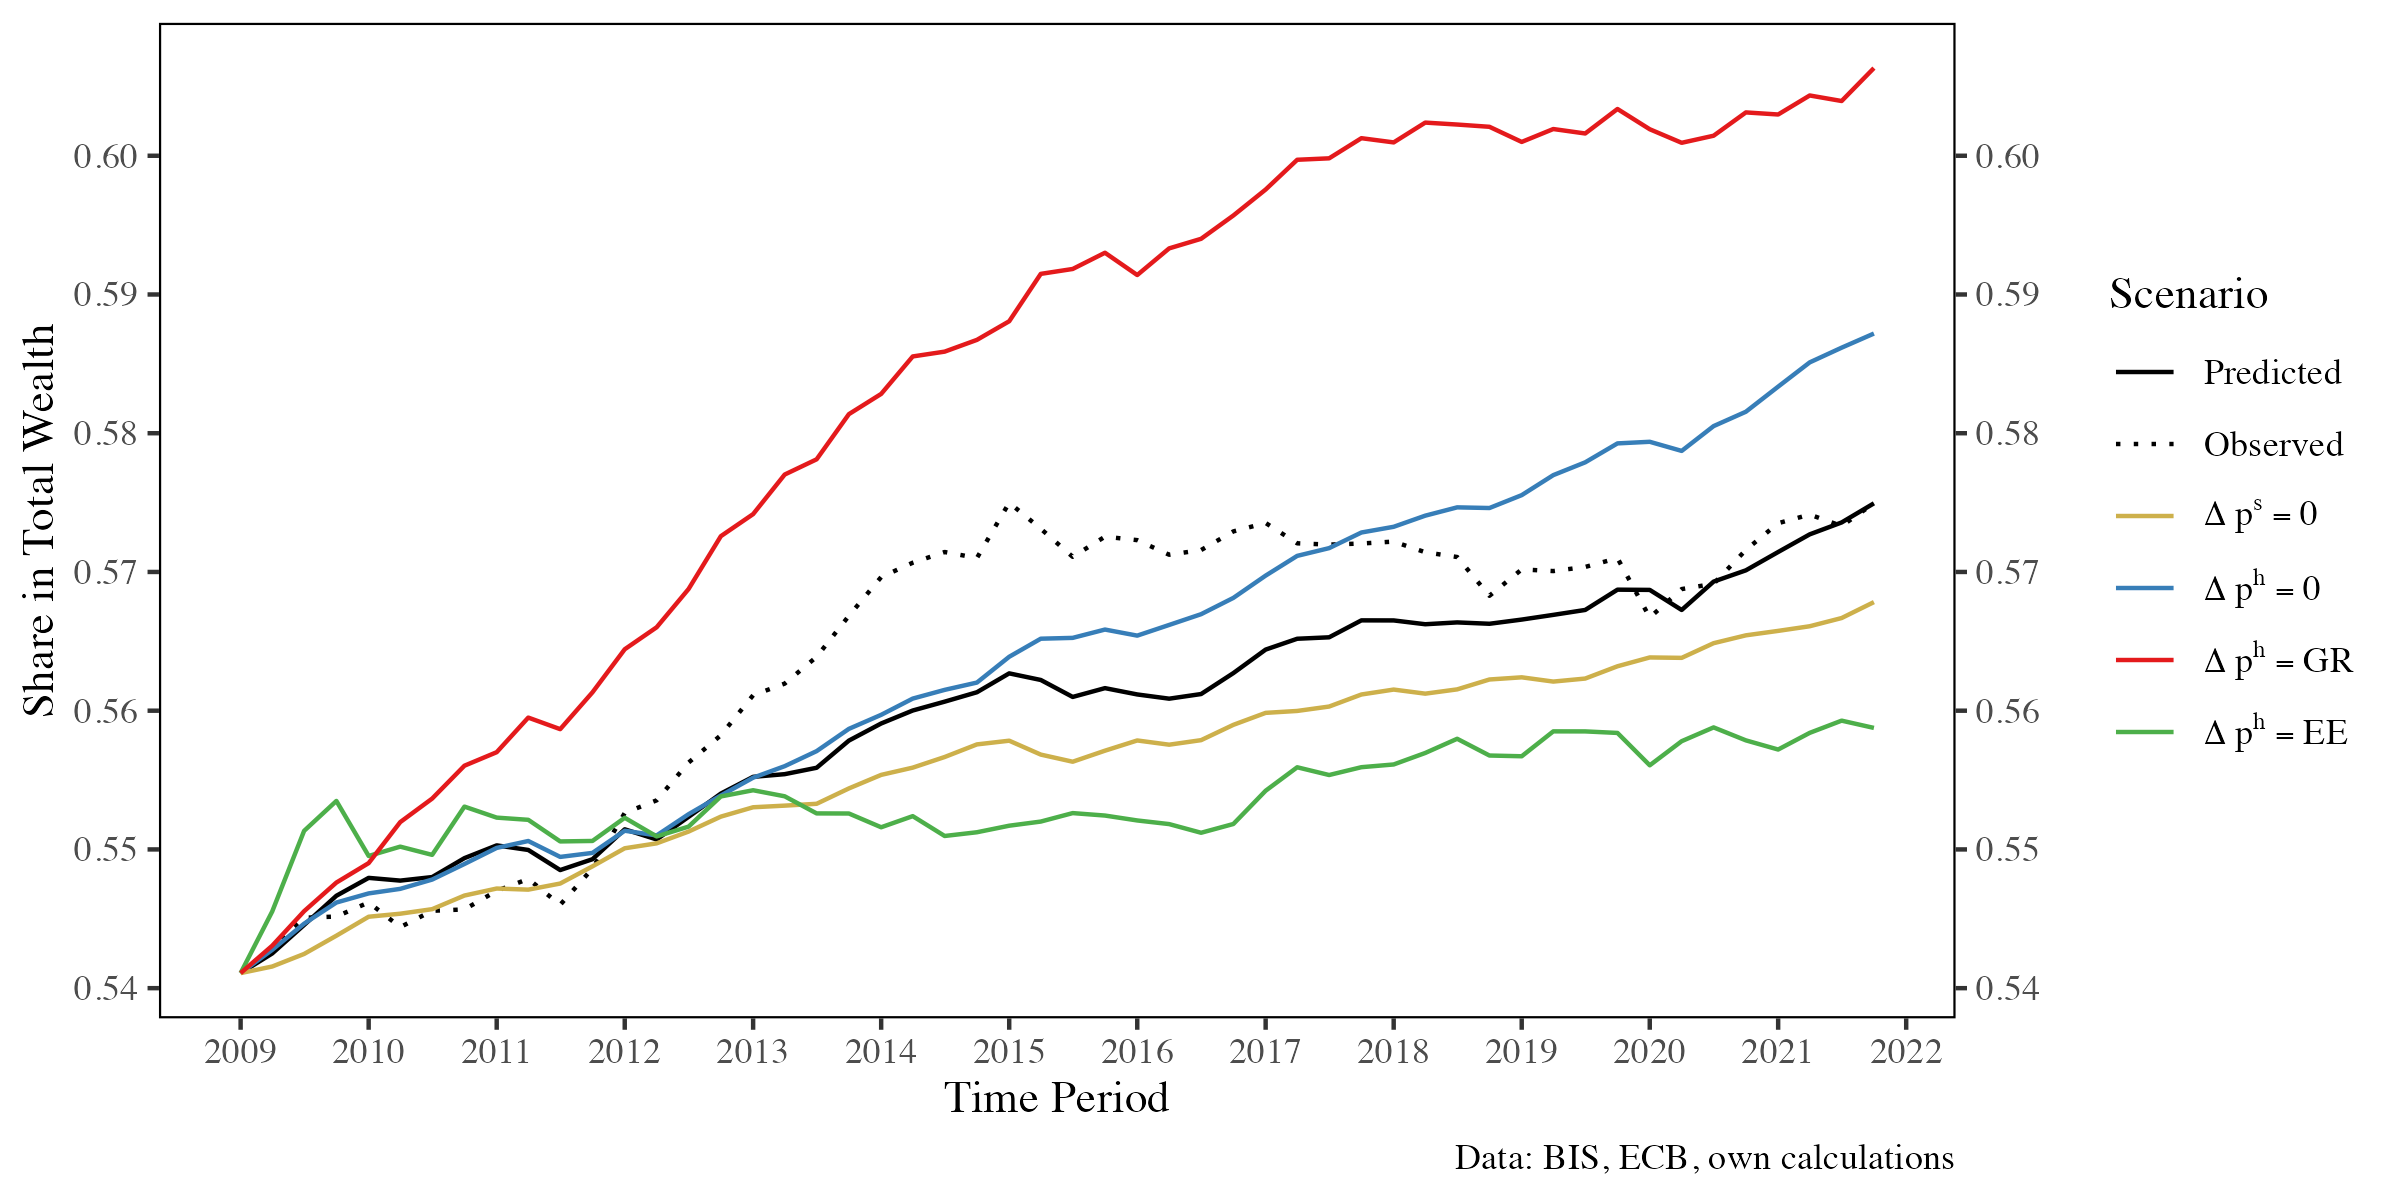
\includegraphics[keepaspectratio]{../output/simulation/counterfactual_T10.png}}

}

\caption{\label{fig-ctfT10}Counterfactual Simulations of top decile
wealth shares}

\end{figure}%

\section{Discussion}\label{sec-discussion}

The empirical results provide a first indication of how asset prices
correlate with changes in wealth distribution across Europe.

One theoretical concern in the regression is reverse causality: rather
than asset prices driving shifts in wealth inequality, it is plausible
that changes in the wealth distribution affect asset price dynamics
themselves. Higher inequality leads to more disposable wealth accruing
at the top, which in turn could lead to more investment in financial
assets and housing, therefore raising prices in a supply-constrained
environment. Goda, Stewart, and Torres García
(\citeproc{ref-godaAbsoluteIncomeInequality2020}{2020}) use
cointegration tests to find that absolute income inequality and housing
prices are positively correlated in OECD countries, suggesting that
inequality itself can fuel price growth.

Given the relatively short time frame of the analysis and its focus on
wealth inequality, it is unlikely that long-run structural shifts in
inequality have been the main driver of housing prices. If the argument
holds, countries with higher inequality at start would have seen a
stronger price increase than the ones with lower inequality.
Empirically, this does not seem to be the case, as presented in Figure
Figure~\ref{fig-reverse} in Appendix G. The relationship between initial
inequality and subsequent housing price growth is weak and inconsistent
across periods. In particular, countries with higher Gini coefficients
in 2014 or 2019 did not systematically experience higher housing price
growth over the following five years.

The literature on drivers of housing prices also emphasises the role of
other exogenous factors (\citeproc{ref-ducaWhatDrivesHouse2021}{Duca,
Muellbauer, and Murphy 2021}). Especially important are financial
constraints, e.g.~interest rates and borrowing regulation, as well as
feedback loops driving endogenous cycles. The authors also stress the
diverse regional trajectories and institutions governing house prices.
In sum, while housing prices clearly drive shifts in housing wealth and
its distribution through the valuation channel, the evidence for a
consistent reverse effect from inequality to price growth is limited in
this context..

Another potential issue is the use of the Stoxx 50 as a stock price
index. As an european average, it cannot capture the individual stock
market conditions in european countries, therefore assuming all
portfolios move in an identical manner.

On the other hand, the broadness of the index ensures that over 60\% of
the european market capitalization is accounted for. Additionally, the
local stock markets in the European Union are highly integrated into the
european market. As Kim, Moshirian, and Wu
(\citeproc{ref-kimDynamicStockMarket2005}{2005}) describes for 15 member
states before 2004 and Savva and Aslanidis
(\citeproc{ref-savvaStockMarketIntegration2010}{2010}) for new member
states after 2004, there are significant comovements of local and
european stock prices. Using local stock indices therefore would not
yield significantly different results and introduce a range of new
problems concerning comparability.

A key limitation of the DWA is that it does not differentiate between
the valuation effect and savings effect when measuring changes in
wealth. An increase in a given groups net wealth could be driven by
changes to the valuation of the existing portfolios as well as increased
savings of households. This is especially important if rising earnings
inequality leads to more disposable income in the upper part of the
wealth distribution, which is invested in assets. Rising Income
Inequality would then lead to a larger share of wealth owned by the top
decile independent of changes in asset valuations.

Kuhn, Schularick, and Steins
(\citeproc{ref-kuhnIncomeWealthInequality2020}{2020}) document the
effects for the US distribution. They find that in the four decades
preceding the 2008 financial crisis, the valuation effect played a
similar role to savings in the development of the wealth distribution
(\citeproc{ref-kuhnIncomeWealthInequality2020}{2020, 41}). It is
especially pronounced for the bottom half, where over 90\% of the groups
wealth growth is induced by changes in the valuation of assets,
especially housing. In the period after the financial crisis, US house
prices plummeted while stock prices quickly rebounded. The authors find
that this led to a stark decrease in wealth owned by the bottom 90\%,
while the top 10\% wealth grew due to the stock prices. As a result, the
US saw the strongest increase in wealth concentration in post-war
history, all the while income inequality remained stable.

In the Eurozone, a similar picture emerges. Wealth inequality increased
over the observed period (2011-2022), while income inequality decreased
slightly (\citeproc{ref-eurostatGiniCoefficientEquivalised2024}{EUROSTAT
2024}). This suggests, that valuation effects are primarily responsible
for the wealth growth, and savings play a smaller role. Furthermore,
given that the temporal frame of the observation is limited to a brief
period, it is more plausible to attribute the increase in net wealth to
asset prices.

In addition to the short-term consequences of asset prices on
inequality, it is important to consider the second-order effects. Rising
house prices without corresponding income increases reduce the
affordability of owning a house, especially for first time buyers. This
could lead to higher wealth inequality in the long term, as lower income
and wealth groups are increasingly excluded from accumulating housing
assets and thus miss out on the associated wealth gains.

Empirical evidence of this phenomenon is presented by C. Bonnet,
Garbinti, and Grobon
(\citeproc{ref-bonnetRisingInequalitiesAccess2019}{2019}) for France.
They find that in the last 40 years, low-income households between 25
and 44 years exhibited a decline in their homeownership rates, with the
reverse for high-income households. In 1973, in the former group 34\% of
households owned their home, while in the latter it was 43\%. This gap
widened in the following decades, with 66\% of the high income group
owning their residence, while the percentage of the low income group
more than halved with 16\%. Notably, the average homeownership rate
remained relatively stable during this period. The authors attribute the
rise in housing inequality to increasing house prices, the subsequent
growing importance of inheritances, and shifts in family structures.

Additionally, rising house prices often translate into higher rents,
further eroding affordability. As Hick, Pomati, and Stephens
(\citeproc{ref-hickHousingAffordabilityPoverty2024}{2024}) document,
housing cost burdens across Europe have become increasingly concentrated
among renters in the private market. Higher rents reduce tenants ability
to save and often prevent the accumulation of wealth, while rental
income flows to landlords, who are disproportionately in the top wealth
deciles. This dynamic also affects first-time buyers as high rents make
it harder to save for mortgage deposits, delaying homeownership and
deepening the divide between those with and without housing wealth.

This divergence between the ``have's'' and ``have-not's'' is described
in Figure~\ref{fig-ratio}. The graph illustrates the growing divide
between tenants and owners across EU countries using the tenant-to-owner
wealth ratio. In many countries the ratio has increased sharply,
indicating that owners have seen much stronger wealth growth relative to
tenants. The largest ratio is measured in Croatia, where home owners own
approximately 20 times as much wealth as tenants, up from 10.23 in the
second quarter of 2017.

\begin{figure}[h]

\centering{

\pandocbounded{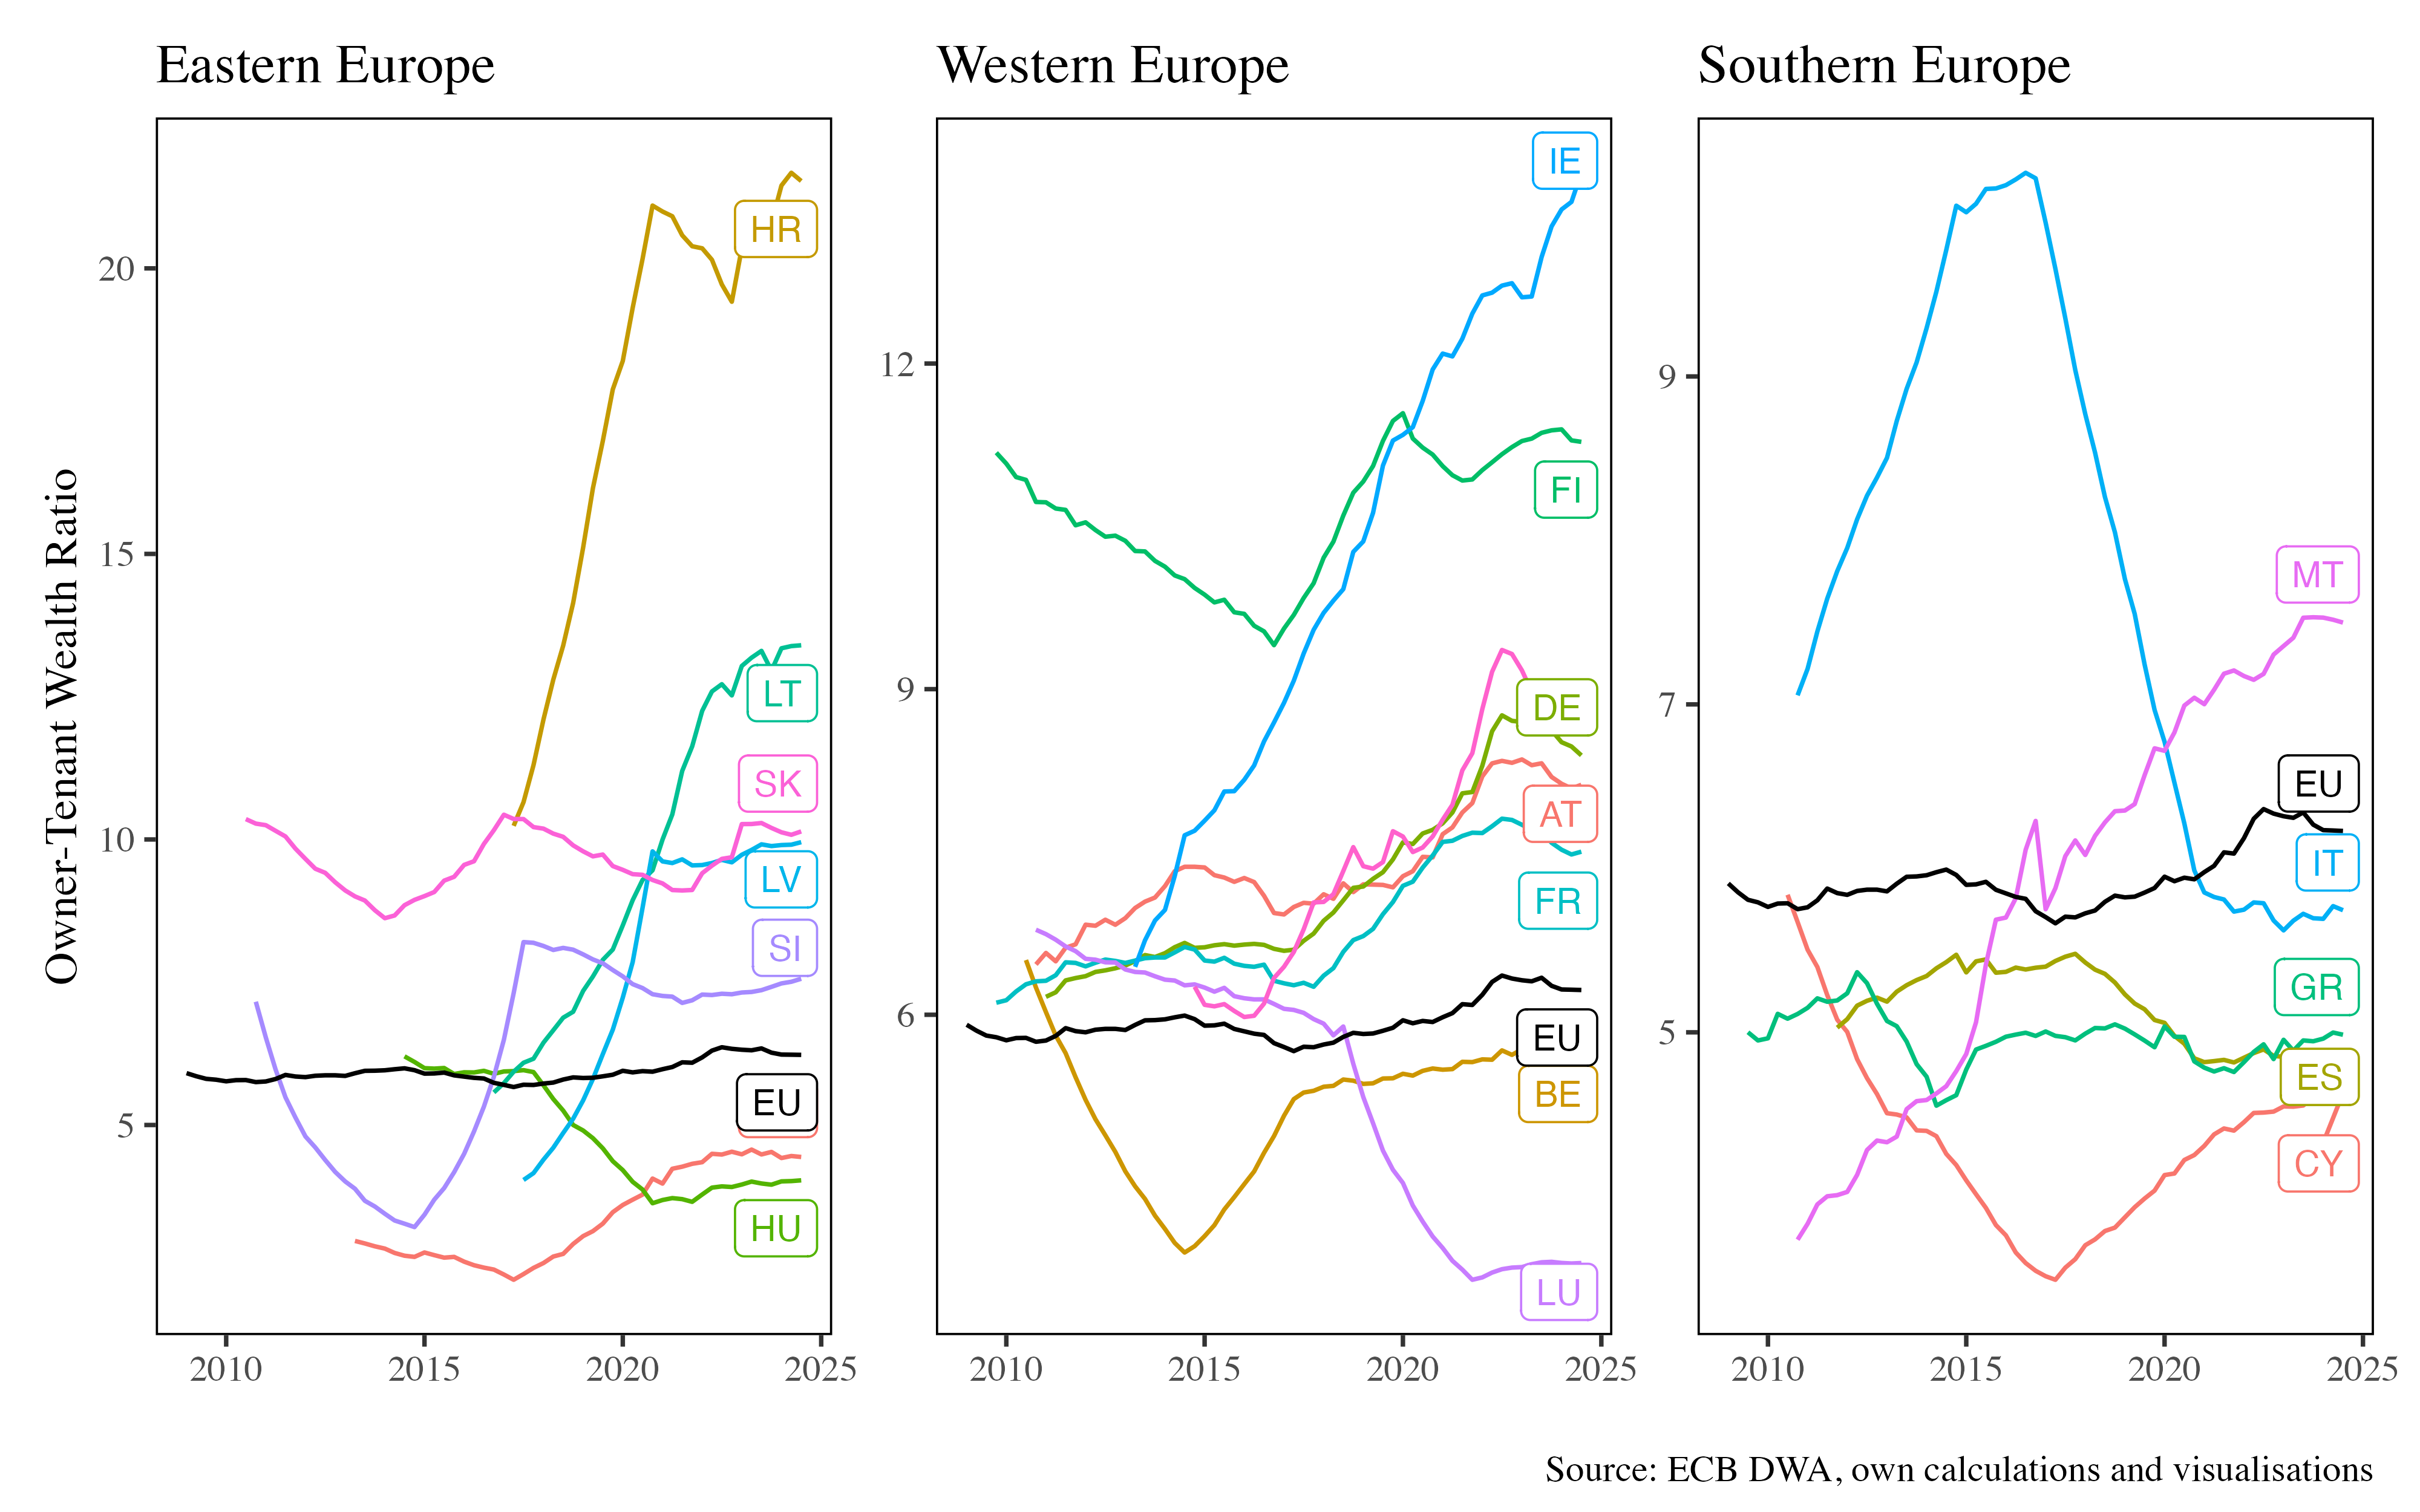
\includegraphics[keepaspectratio]{../output/desc/tenant_owner_wealth_ratio_europe.png}}

}

\caption{\label{fig-ratio}Owner-Tenant Wealth Ratios}

\end{figure}%

This aligns with the argument proposed by Kaas, Kocharkov, and
Preugschat (\citeproc{ref-kaasWealthInequalityHomeownership2019}{2019}),
who employed a decomposition approach to analyze european wealth Gini
coefficients, distinguishing between owner and tenant groups. Their
analysis revealed that the between-group component contributed
significantly to the overall inequality observed
(\citeproc{ref-kaasWealthInequalityHomeownership2019}{2019, 34}).

Wealth share responses estimated in this thesis are also relevant in the
context of monetary policy, particularly given the strong influence of
monetary interventions on asset prices. Conventional policy tools, such
as interest rate cuts, are known to increase equity valuations
(\citeproc{ref-bernankeWhatExplainsStock2005}{Bernanke and Kuttner
2005}). Housing markets respond similarly: contractionary shocks have
been shown to lower house prices in Europe
(\citeproc{ref-coenMonetaryShocksHouse2024}{Coën and Pourcelot 2024}),
although the effect is highly heterogeneous across countries
(\citeproc{ref-battistiniNavigatingHousingChannel2025}{Battistini et al.
2025}).

The observation period of this thesis (2011--2022) overlaps with a phase
of historically low interest rates, the Eurozone sovereign debt crisis,
and the ECB's shift toward unconventional monetary policy. This included
large-scale purchases of corporate and government securities, boosting
equity prices, which quickly rebounded
(\citeproc{ref-fratzscherECBUnconventionalMonetary2016}{Fratzscher, Lo
Duca, and Straub 2016}). House prices on the other hand plateaud until
2015, before rising, albeit much slower than stock prices.

Thus decisions taken in light of the euro crisis had direct consequences
on the wealth distribution in Europe. Higher stock prices, coupled with
stable house prices, resulted in an increase in capital gains for the
top decile, while the rest of the population did not benefit in a
similar fashion. Bernoth, König, and Beckers
(\citeproc{ref-bernothECBAssetPurchases2016}{2016}) described this
theoretical consequence of the ECB purchasing programs, and more
detailed empirical research on the heterogenous distributional effects
is needed to incorporate it into monetary policy frameworks.

One question that arises from the individual results is why portfolios
and subsequent reactions to asset price movements differ so strongly
across Europe. What institutional and cultural differences explain the
large variance?

Research points into the direction of home ownership as a central
explanatory power. Mathä, Porpiglia, and Ziegelmeyer
(\citeproc{ref-mathaHouseholdWealthEuro2017}{2017}) find that the home
ownership rate in addition to house price dynamics explain more than
50\% of the wealth differences in Europe, particularly in the middle
part of the distribution. Similarly, Kaas, Kocharkov, and Preugschat
(\citeproc{ref-kaasWealthInequalityHomeownership2019}{2019}) highlight
that home ownership rates are strongly negatively related to wealth
inequality in the 9 largest european countries. The authors also stress
that the home ownership rate itself is higly endogenous and variations
have to be explained by institutional and cultural differences.

Several institutions influencing home ownership decisions are analysed
in the literature (for an overview see
\citeproc{ref-bourassaDeterminantsHomeownershipRate2015}{Bourassa et al.
2015}). Cho and Francis (\citeproc{ref-choTaxTreatmentOwner2011}{2011})
focus on preferential tax treatment in the form of mortgage interest
rate deductibility and missing taxation of imputed rents. They find that
it provides a financial incentive to own instead of rent in the US case
and has negative distributional effects.

Kaas, Kocharkov, and Preugschat
(\citeproc{ref-kaasWealthInequalityHomeownership2019}{2019})
additionally highlight the role of sales tax on homes and average
downpayment requirements, which differ across Europe and explain part of
the variation in homeownership rates. In a companion paper
(\citeproc{ref-kaasLowHomeownershipGermany2021}{Kaas et al. 2021}), the
authors incorporate these factors into a structural model to explain the
low german homeownership rate. Running counterfactual experiments, they
show that reducing transfer taxes and implementing mortgage interest
rate deductions would increase the share of homeowners, while reducing
welfare, particularly for new entrants into the housing market.

Therefore, it is important to note that while a higher homeownership
rate may lead to a more equitable distribution of wealth, it also
introduces consequences regarding market efficiency and distribution. In
addition to upper-income classes profiting more if the higher rate is
achieved through preferential tax treatment, it also creates an
incentive to over consume housing as an asset
(\citeproc{ref-choTaxTreatmentOwner2011}{Cho and Francis 2011}). This
creates a ``lock in'' effect for owners, decreasing residential mobility
with adverse effects on the functioning of the labor market
(\citeproc{ref-causaHousingWealthAccumulation2019}{Causa, Woloszko, and
Leite 2019}).

Beyond differences in homeownership rates, variation in household
leverage is another key factor shaping how housing price changes affect
wealth inequality. As noted by Causa, Woloszko, and Leite
(\citeproc{ref-causaHousingWealthAccumulation2019}{2019}), there is
substantial heterogeneity in household leverage, particularly housing
debt. In some countries, such as the Netherlands and Ireland, average
loan-to-value ratios exceed 50\%, with high leverage especially common
in the lower part of the wealth distribution. This can amplify gains
when house prices increase, but also exposes households to significant
risks if prices fall or if interest rates rise, particularly in markets
with variable-rate mortgages.

Such differences in leverage profiles could help explain part of the
cross-country heterogeneity in wealth share reactions found in the
regressions. While Martínez-Toledano
(\citeproc{ref-martinez-toledanoHousePriceCycles2022}{2022}) touches on
these dynamics for Spain
(\citeproc{ref-martinez-toledanoHousePriceCycles2022}{2022, 19}),
broader evidence for other European countries remains scarce. The DWA,
with its coverage of housing and other forms of debt across all wealth
deciles, offers a promising basis for extending this line of research.

Taken together, the discussion highlights the importance of asset
prices, especially housing and equities, in shaping recent wealth
dynamics across Europe. While short-term valuation effects appear to
drive much of the observed inequality, their distributional consequences
are mediated by national institutions, ownership structures, and policy
regimes. The analysis also points to monetary policy as an indirect but
powerful driver of wealth inequality, raising questions about the
distributive impact of asset purchases and interest rate decisions.
Given the data limitations and focus on a relatively short time frame,
further research is needed to disentangle long-run structural drivers
from cyclical price effects, and to assess how policy interventions can
be designed to mitigate wealth concentration.

\section{Conclusion}\label{sec-conclusion}

This thesis examined how wealth inequality in Europe responds to changes
in asset prices. The analysis reveals clear and distinct patterns: the
middle and lower parts of the distribution profit from increases in
house prices, while the top decile benefits predominantly from growth in
stock prices.

The results carry important implications for both housing and monetary
policy. Housing market regimes determine who is able to take part in the
property ladder, while monetary policy decisions shape asset valuations
and, through them, the distribution of wealth. Understanding these
channels is essential for assessing the wider consequences of policy
interventions in both areas.

The literature on the determinants of wealth inequality identifies asset
prices as a central factor, with housing playing a particularly
important role. This thesis contributes to that work by using
higher-frequency, macro-consistent data from the ECB's novel
Distributional Wealth Accounts, allowing a closer examination of
short-term changes in wealth shares. The results confirm that valuation
effects are a key part of wealth dynamics.

This work yields several avenues for future research. One is to further
decompose the role of savings and valuation effects, as well as how they
intertwine. Additionally, the role of leverage in shaping wealth
distribution has not been well-reported until now, and the DWA opens up
multiple avenues for this. Further analysis is also needed to explain
the heterogeneous effects of asset prices at the country-specific level.

\newpage{}

\section*{Appendix}\label{appendix}
\addcontentsline{toc}{section}{Appendix}

\subsection*{Appendix A: Housing Wealth across
Europe}\label{appendix-a-housing-wealth-across-europe}
\addcontentsline{toc}{subsection}{Appendix A: Housing Wealth across
Europe}

\begin{figure}[h]

\centering{

\pandocbounded{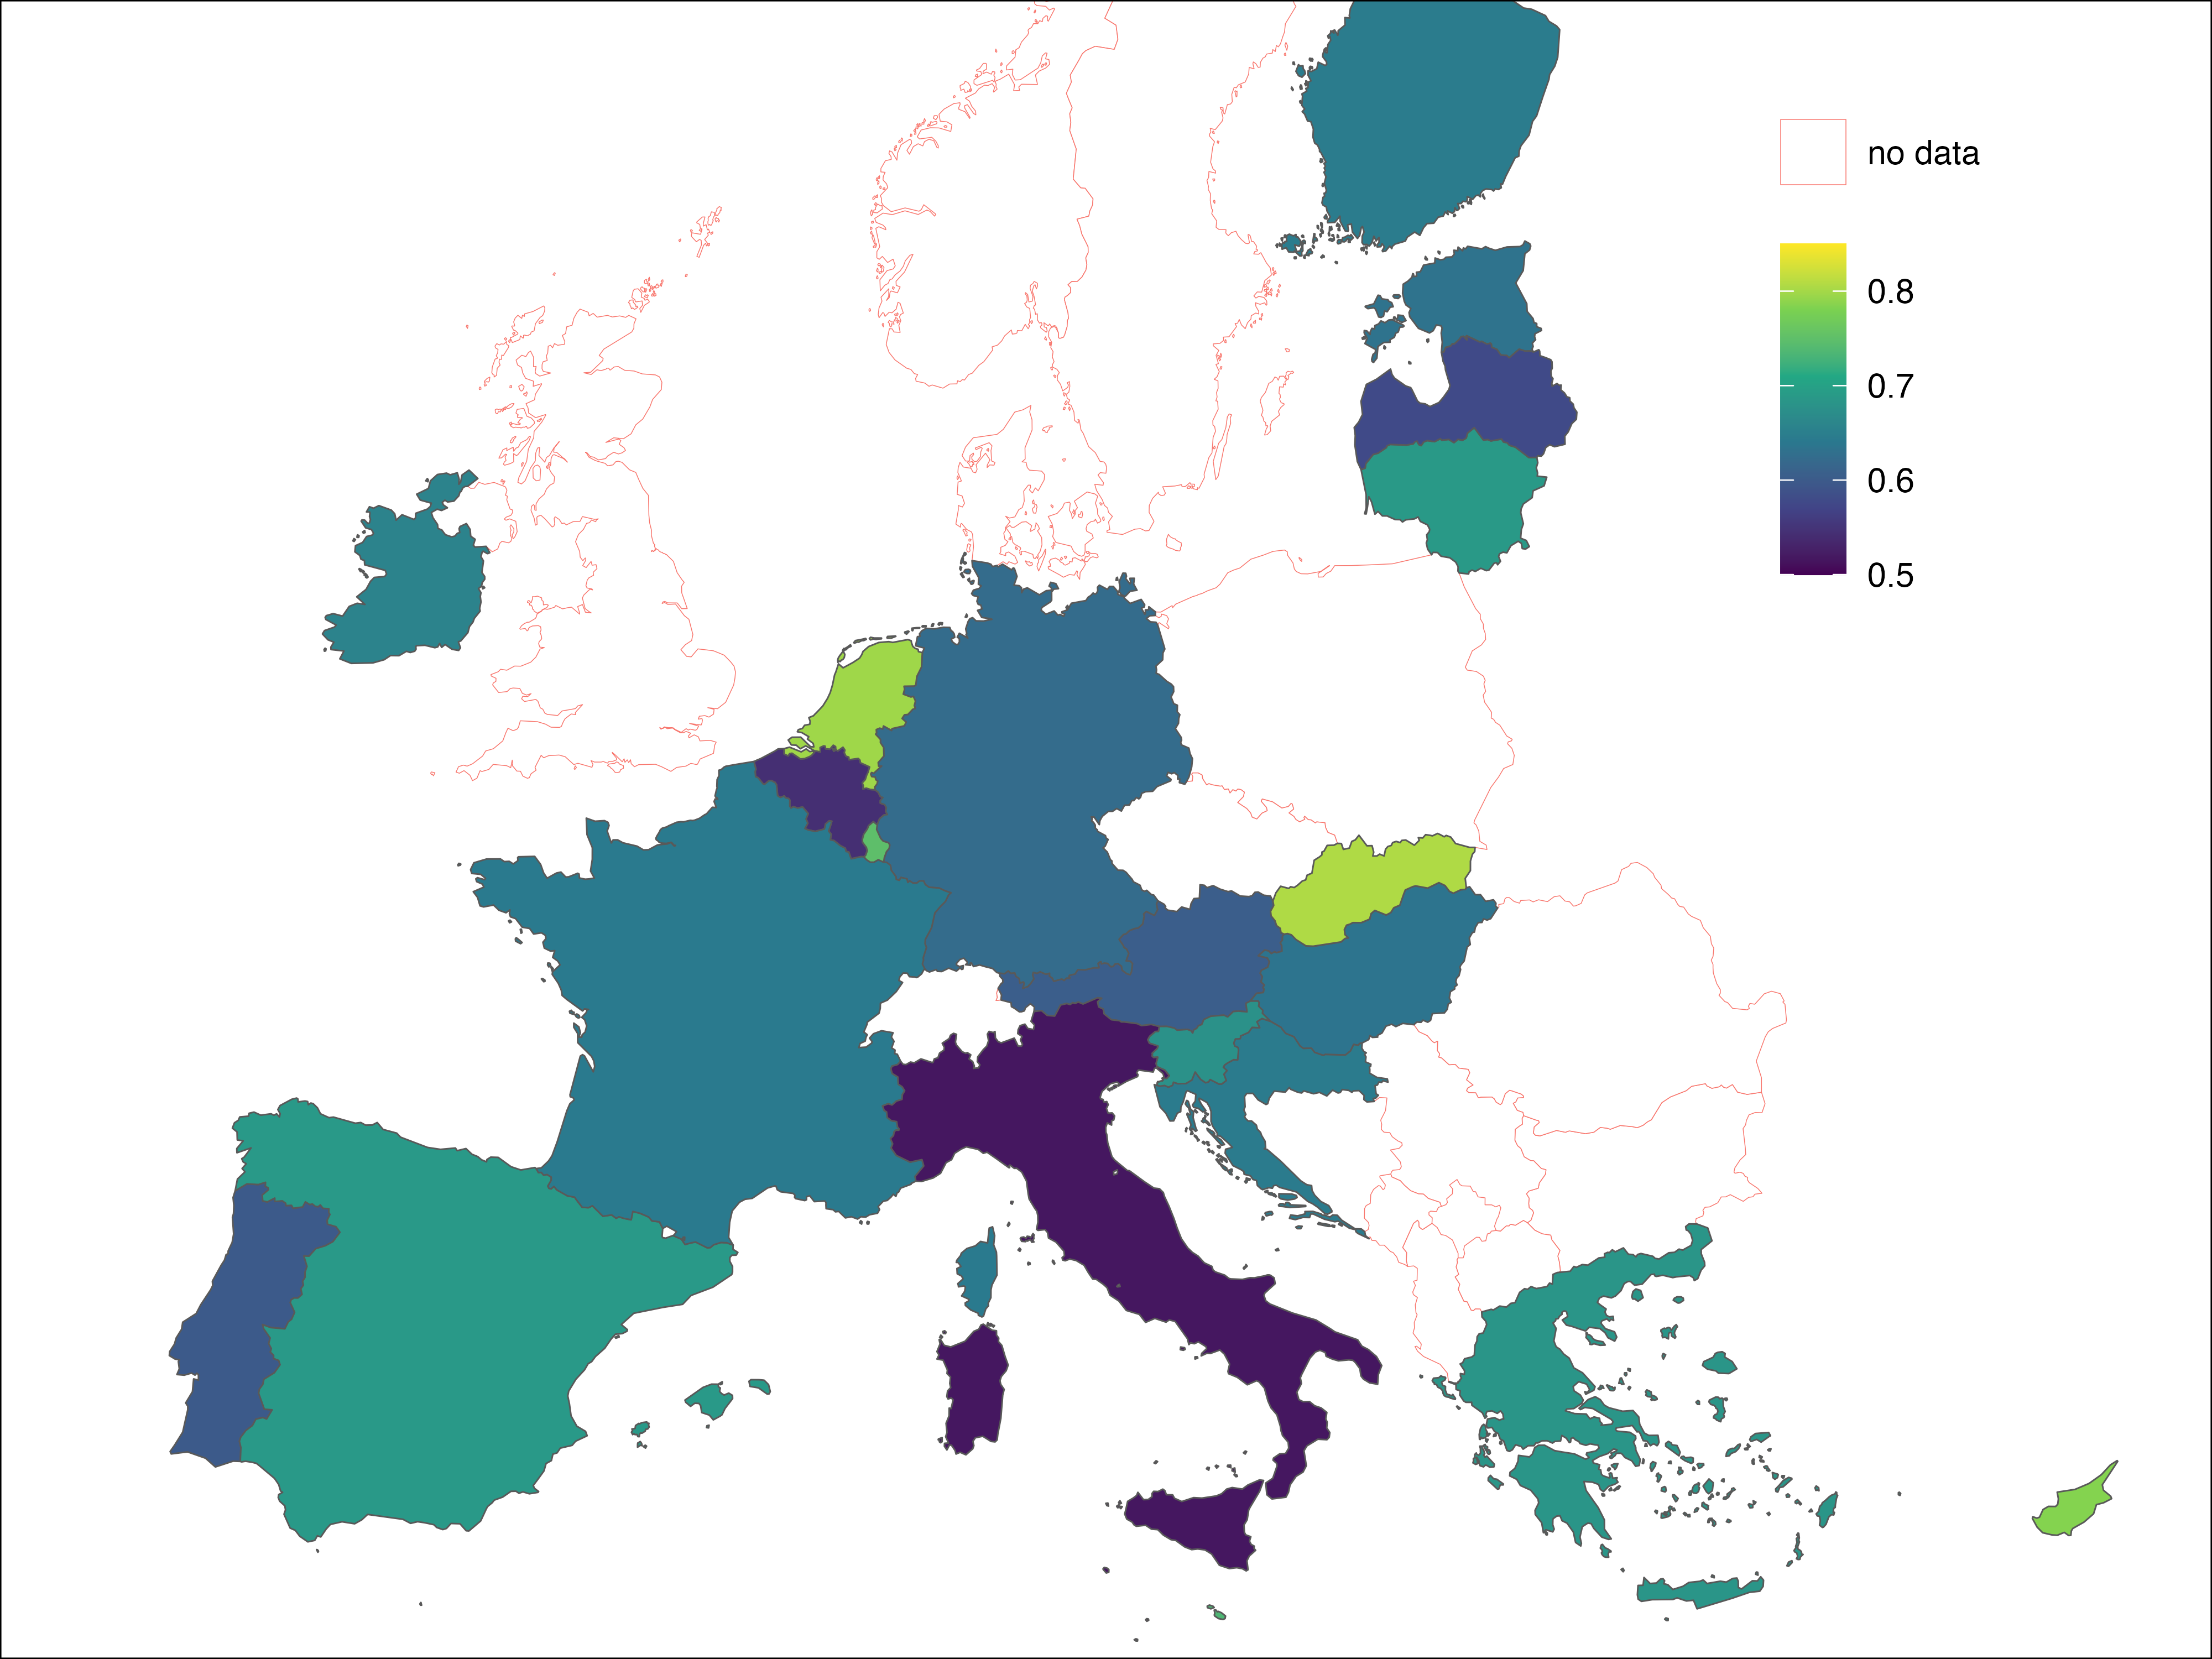
\includegraphics[keepaspectratio]{../output/desc/map.png}}

}

\caption{\label{fig-map}Housing wealth as share of total net wealth}

\end{figure}%

\newpage{}

\subsection*{Appendix B: Descriptive
Table}\label{appendix-b-descriptive-table}
\addcontentsline{toc}{subsection}{Appendix B: Descriptive Table}

The following Table presents the full country names and the net wealth
per Capita in Euro in 2022.

\begin{table}[h]

\caption{\label{tbl-descriptive}Descriptive Table with ISO 2 Codes}

\begin{minipage}{\linewidth}

\fontsize{10.0pt}{12.0pt}\selectfont
\begin{tabular*}{\linewidth}{@{\extracolsep{\fill}}llccrr}
\toprule
\multicolumn{2}{c}{Name} & \multicolumn{2}{c}{Time Period} & \multicolumn{2}{c}{Net Wealth (EUR p.C)} \\ 
\cmidrule(lr){1-2} \cmidrule(lr){3-4} \cmidrule(lr){5-6}
ISO2 & Full Name & Start & End & Mean & Median \\ 
\midrule\addlinespace[2.5pt]
AT & Austria & 2010 Q4 & 2024 Q3 & 213570 & 148200 \\ 
BE & Belgium & 2010 Q3 & 2024 Q3 & 254570 & 288469 \\ 
CY & Cyprus & 2010 Q3 & 2024 Q3 & 200490 & 358090 \\ 
DE & Germany & 2011 Q1 & 2024 Q3 & 221080 & 118634 \\ 
EE & Estonia & 2013 Q2 & 2024 Q3 & 94850 & 92574 \\ 
ES & Spain & 2011 Q4 & 2024 Q3 & 175130 & 202247 \\ 
FI & Finland & 2009 Q4 & 2024 Q3 & 165160 & 129728 \\ 
FR & France & 2009 Q4 & 2024 Q3 & 198810 & 175016 \\ 
GR & Greece & 2009 Q3 & 2024 Q3 & 89890 & 131323 \\ 
HR & Croatia & 2017 Q2 & 2024 Q3 & 39023 & 40130 \\ 
HU & Hungary & 2014 Q3 & 2024 Q3 & 73370 & 86680 \\ 
EU & Eurozone & 2009 Q1 & 2024 Q3 & 182787 & 152275 \\ 
IE & Ireland & 2013 Q2 & 2024 Q3 & 251940 & 357059 \\ 
IT & Italy & 2010 Q4 & 2024 Q3 & 180390 & 158171 \\ 
LT & Lithuania & 2016 Q4 & 2024 Q3 & 75990 & 69192 \\ 
LU & Luxembourg & 2010 Q4 & 2024 Q3 & 606820 & 759153 \\ 
LV & Latvia & 2017 Q3 & 2024 Q3 & 36900 & 27821 \\ 
MT & Malta & 2010 Q4 & 2024 Q3 & 270420 & 414803 \\ 
NL & Netherlands & 2014 Q4 & 2023 Q4 & 396990 & 215032 \\ 
PT & Portugal & 2010 Q2 & 2024 Q3 & 114100 & 125440 \\ 
SI & Slovenia & 2010 Q4 & 2024 Q3 & 119880 & 160980 \\ 
SK & Slovakia & 2010 Q3 & 2024 Q3 & 56080 & 101871 \\ 
\bottomrule
\end{tabular*}

\end{minipage}%

\end{table}%

\subsection*{Appendix C: Portfolio and Asset Distribution across
Europe}\label{appendix-c-portfolio-and-asset-distribution-across-europe}
\addcontentsline{toc}{subsection}{Appendix C: Portfolio and Asset
Distribution across Europe}

The following figures describe Asset Distribution as well as Portfolio
Composition across Europe using the latest quarter of 2021.

\begin{figure}[H]

\centering{

\pandocbounded{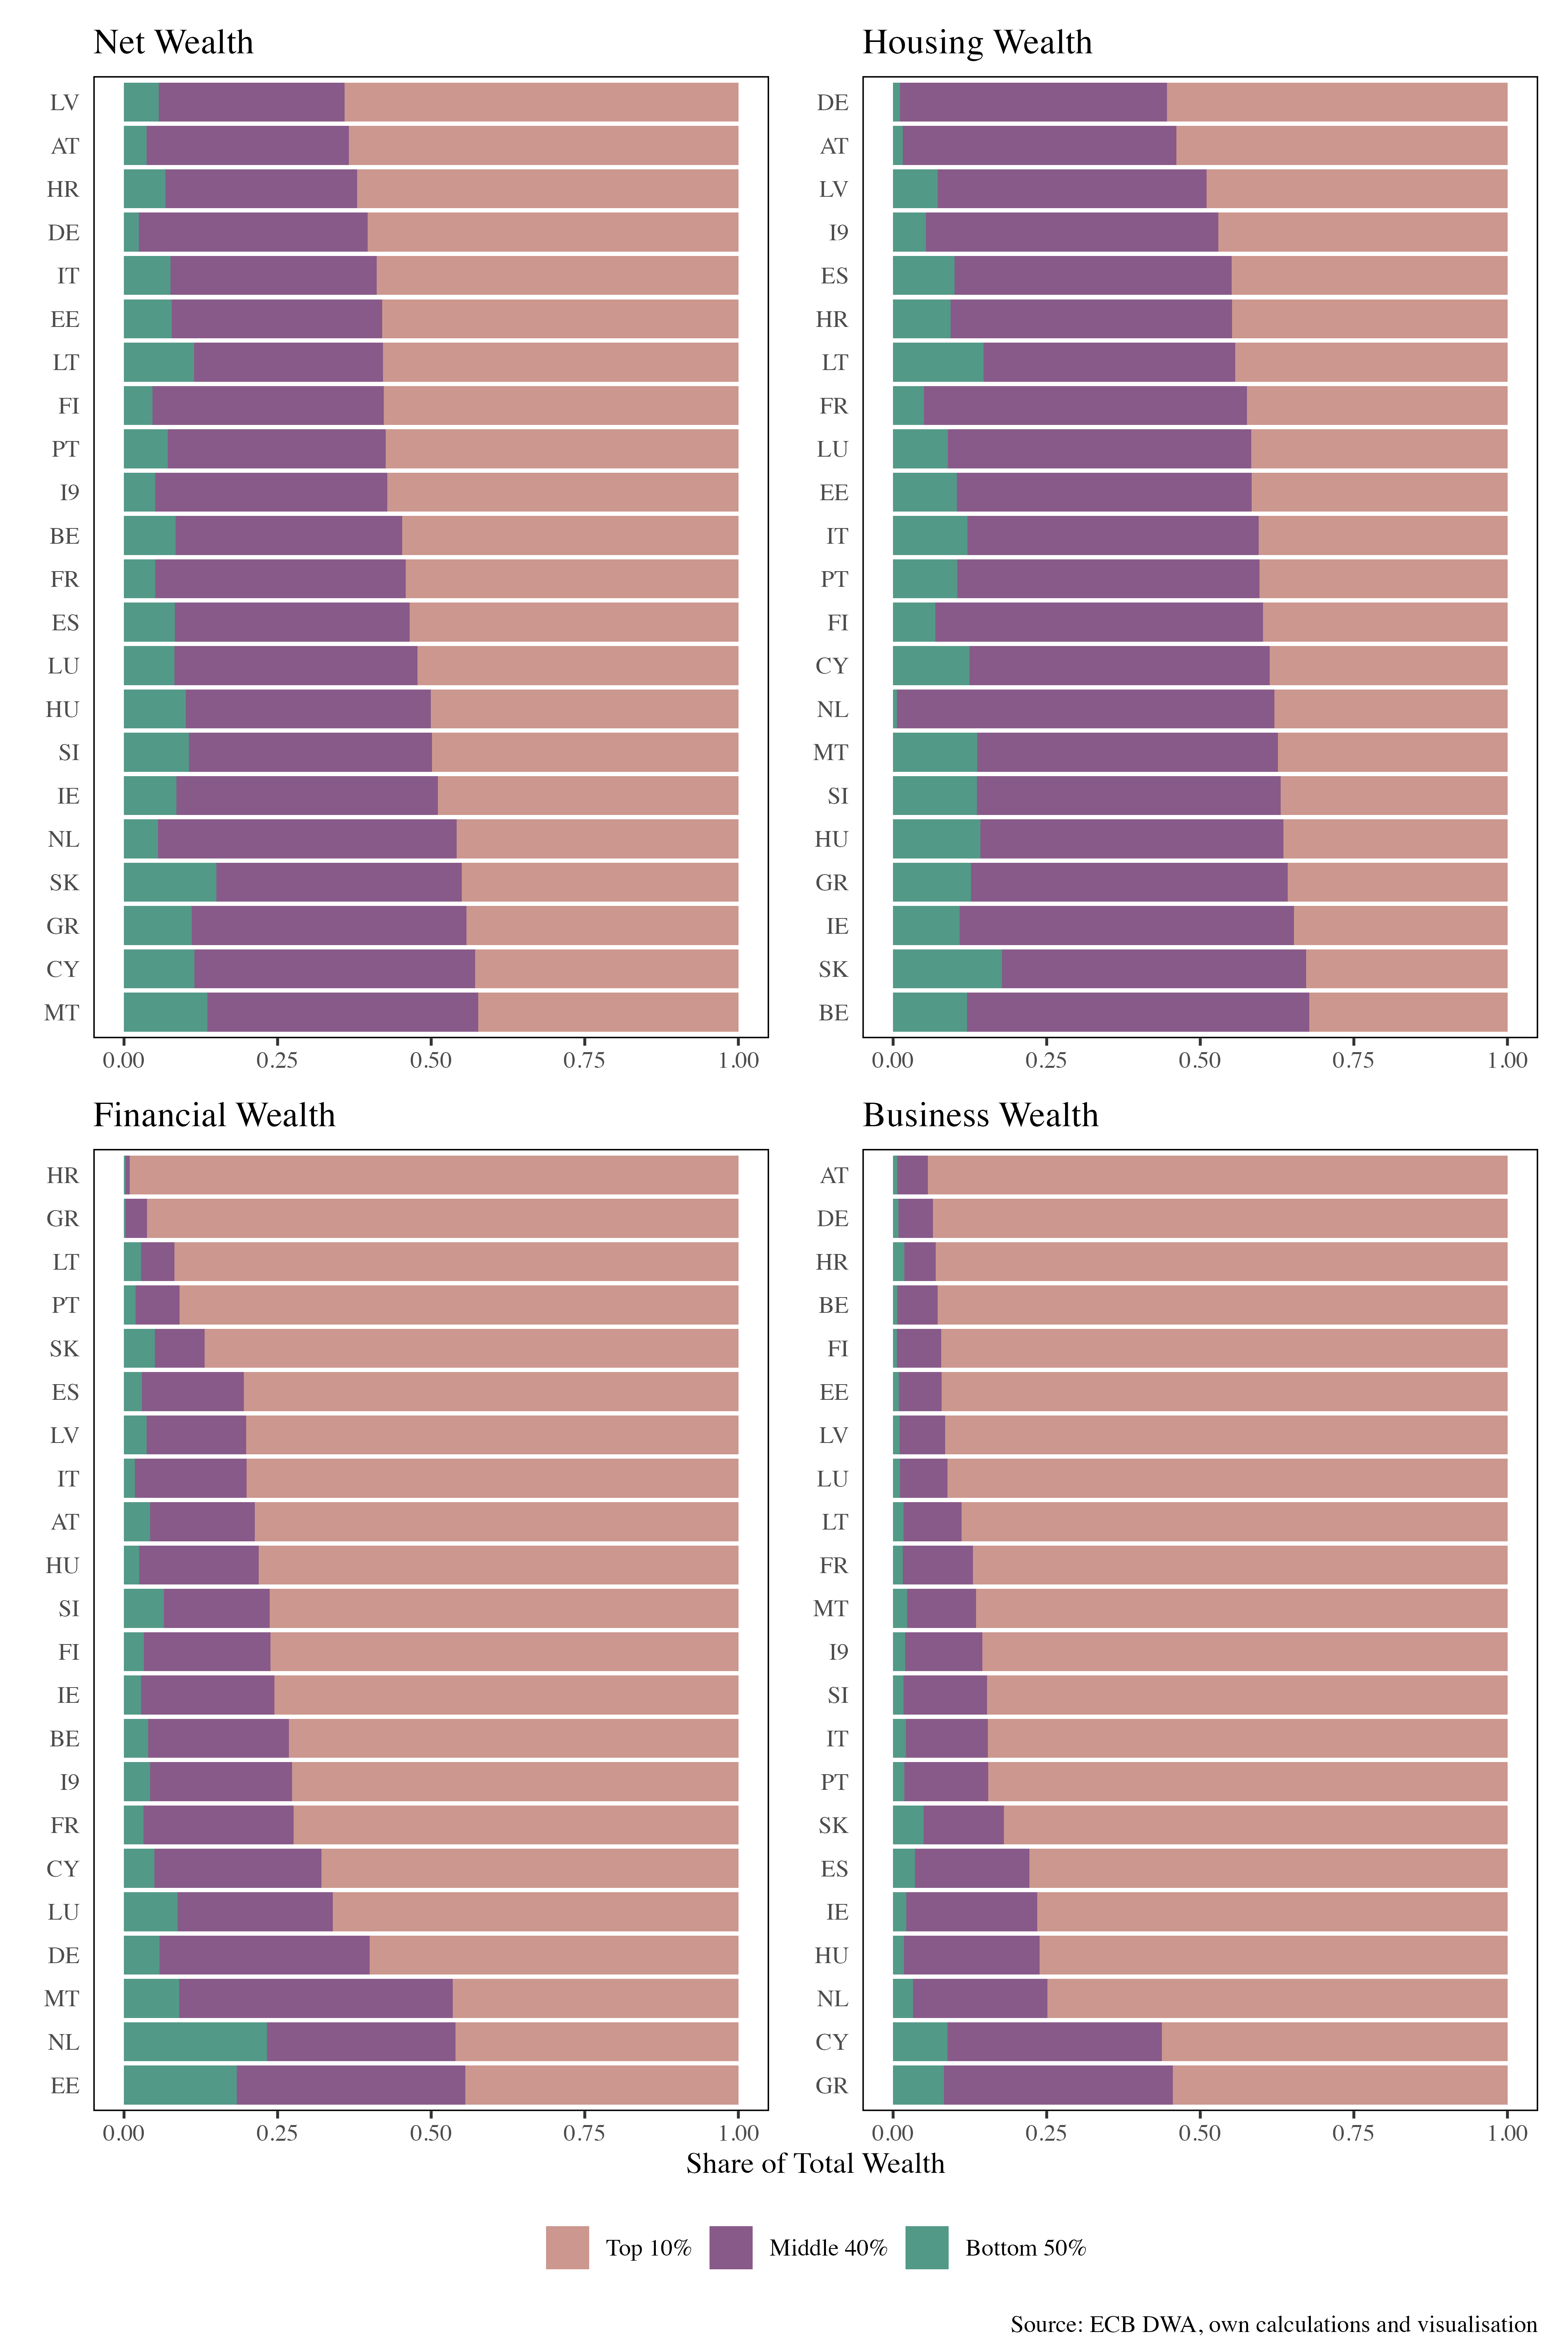
\includegraphics[keepaspectratio]{../output/appendix/asset_distribution_individual.png}}

}

\caption{\label{fig-distribution-indiv}Asset Distribution among Deciles}

\end{figure}%

\begin{figure}[H]

\centering{

\pandocbounded{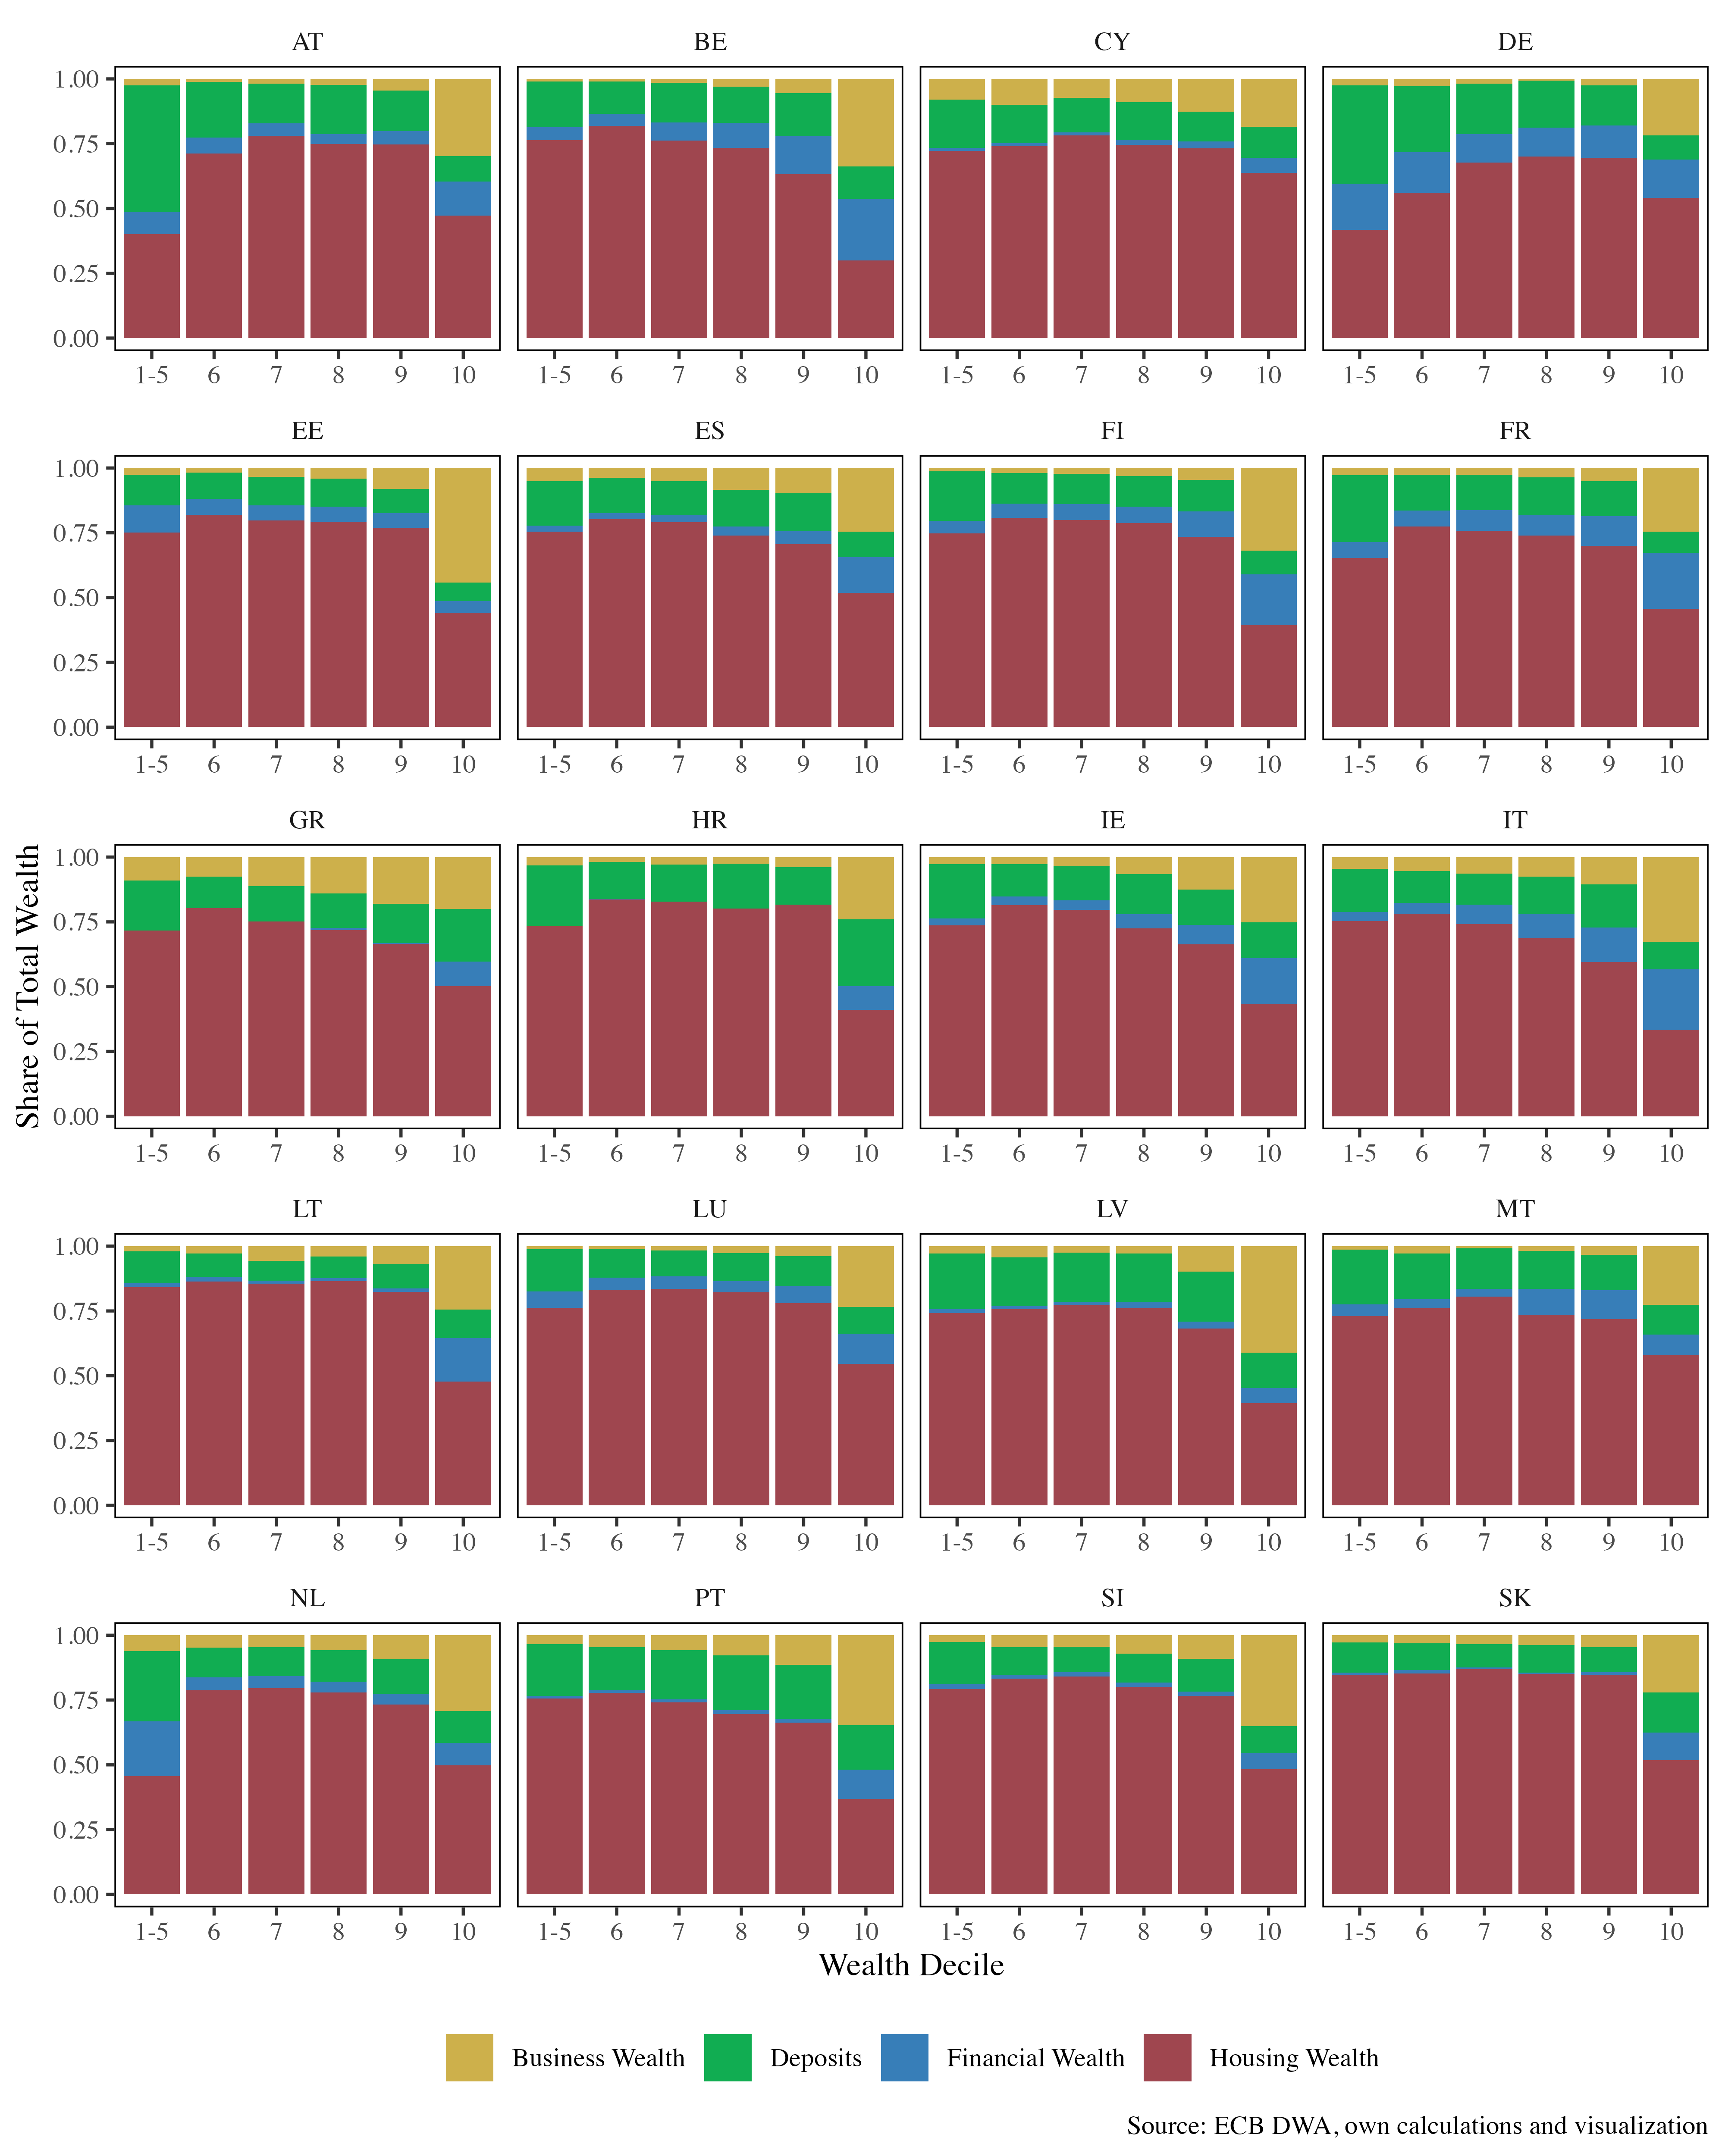
\includegraphics[keepaspectratio]{../output/appendix/portfolios.png}}

}

\caption{\label{fig-portfolio-indiv}Portfolio Composition of Deciles}

\end{figure}%

\subsection*{Appendix D: Individual regressions
results}\label{appendix-d-individual-regressions-results}
\addcontentsline{toc}{subsection}{Appendix D: Individual regressions
results}

\begin{landscape}

\begin{table}[h]
\caption{Top 10\%: Individual regressions} 
\fontsize{7.5pt}{9.0pt}\selectfont
\begin{tabular*}{\linewidth}{@{\extracolsep{\fill}}lccccccccccc}
\toprule
  & AT & BE & CY & DE & EE & ES & FI & FR & GR & HR & HU \\ 
\midrule\addlinespace[2.5pt]
House Prices & -0.078*** & -0.101* & 0.032 & -0.095 & -0.137*** & -0.198*** & -0.053 & -0.134*** & -0.037 & -0.090*** & -0.112* \\ 
 & (0.021) & (0.057) & (0.038) & (0.068) & (0.033) & (0.032) & (0.040) & (0.022) & (0.031) & (0.021) & (0.058) \\ 
Stock Prices & 0.013* & 0.014** & -0.005 & 0.012 & -0.010 & 0.029*** & 0.021*** & 0.032*** & 0.034*** & -0.010 & 0.011 \\ 
{} & {(0.007)} & {(0.006)} & {(0.012)} & {(0.009)} & {(0.018)} & {(0.011)} & {(0.006)} & {(0.006)} & {(0.009)} & {(0.008)} & {(0.023)} \\ 
N & 44 & 45 & 45 & 43 & 34 & 40 & 48 & 48 & 49 & 18 & 29 \\ 
R² & 0.214 & 0.136 & 0.016 & 0.090 & 0.196 & 0.491 & 0.138 & 0.366 & 0.137 & 0.044 & 0.069 \\ 
Adj. R² & 0.176 & 0.095 & -0.031 & 0.045 & 0.144 & 0.463 & 0.100 & 0.337 & 0.100 & -0.084 & -0.002 \\ 
\bottomrule
\end{tabular*}
\begin{minipage}{\linewidth}
* p < 0.1, ** p < 0.05, *** p < 0.01\\
Standard errors estimated following Newey and West (1987)\\
\end{minipage}
\end{table}




\begin{table}[h]
\fontsize{7.5pt}{9.0pt}\selectfont
\begin{tabular*}{\linewidth}{@{\extracolsep{\fill}}lcccccccccc}
\toprule
  & IE & IT & LT & LU & LV & MT & NL & PT & SI & SK \\ 
\midrule\addlinespace[2.5pt]
House Prices & -0.107 & -0.069 & 0.036 & -0.058** & 0.095*** & -0.051 & 0.189*** & -0.072*** & -0.139*** & 0.010 \\ 
 & (0.069) & (0.073) & (0.071) & (0.027) & (0.027) & (0.037) & (0.042) & (0.027) & (0.028) & (0.086) \\ 
Stock Prices & 0.027 & 0.050*** & -0.032** & 0.006 & -0.013 & 0.019 & 0.046*** & 0.023*** & 0.008 & 0.013 \\ 
{} & {(0.023)} & {(0.009)} & {(0.014)} & {(0.006)} & {(0.013)} & {(0.021)} & {(0.007)} & {(0.008)} & {(0.010)} & {(0.020)} \\ 
N & 34 & 44 & 20 & 44 & 17 & 44 & 28 & 46 & 44 & 45 \\ 
R² & 0.072 & 0.298 & 0.139 & 0.111 & 0.246 & 0.042 & 0.333 & 0.165 & 0.291 & 0.011 \\ 
Adj. R² & 0.012 & 0.264 & 0.038 & 0.067 & 0.139 & -0.004 & 0.279 & 0.127 & 0.256 & -0.036 \\ 
\bottomrule
\end{tabular*}
\begin{minipage}{\linewidth}
* p < 0.1, ** p < 0.05, *** p < 0.01\\
Standard errors estimated following Newey and West (1987)\\
\end{minipage}
\end{table}




\end{landscape}

\newpage{}

\begin{landscape}

\begin{table}[h]
\caption{Middle 40\%: Individual regressions} 
\fontsize{7.5pt}{9.0pt}\selectfont
\begin{tabular*}{\linewidth}{@{\extracolsep{\fill}}lccccccccccc}
\toprule
  & AT & BE & CY & DE & EE & ES & FI & FR & GR & HR & HU \\ 
\midrule\addlinespace[2.5pt]
House Prices & 0.114*** & 0.107 & -0.074*** & 0.115 & 0.121*** & 0.085*** & 0.001 & 0.128*** & -0.024 & 0.118** & 0.076 \\ 
 & (0.037) & (0.069) & (0.023) & (0.100) & (0.038) & (0.028) & (0.047) & (0.033) & (0.036) & (0.051) & (0.074) \\ 
Stock Prices & -0.020 & -0.016* & -0.001 & -0.022 & -0.002 & -0.031*** & -0.032*** & -0.034*** & -0.032*** & 0.023 & -0.017 \\ 
{} & {(0.013)} & {(0.009)} & {(0.008)} & {(0.015)} & {(0.024)} & {(0.010)} & {(0.007)} & {(0.008)} & {(0.007)} & {(0.016)} & {(0.029)} \\ 
N & 44 & 45 & 45 & 43 & 34 & 40 & 48 & 48 & 49 & 18 & 29 \\ 
R² & 0.182 & 0.098 & 0.090 & 0.085 & 0.147 & 0.266 & 0.171 & 0.294 & 0.155 & 0.030 & 0.027 \\ 
Adj. R² & 0.142 & 0.055 & 0.047 & 0.039 & 0.092 & 0.227 & 0.134 & 0.263 & 0.118 & -0.099 & -0.048 \\ 
\bottomrule
\end{tabular*}
\begin{minipage}{\linewidth}
* p < 0.1, ** p < 0.05, *** p < 0.01\\
Standard errors estimated following Newey and West (1987)\\
\end{minipage}
\end{table}




\begin{table}[h]
\fontsize{7.5pt}{9.0pt}\selectfont
\begin{tabular*}{\linewidth}{@{\extracolsep{\fill}}lcccccccccc}
\toprule
  & IE & IT & LT & LU & LV & MT & NL & PT & SI & SK \\ 
\midrule\addlinespace[2.5pt]
House Prices & 0.022 & 0.032 & -0.095 & -0.007 & -0.046 & -0.010 & -0.112* & 0.002 & 0.094*** & -0.057 \\ 
 & (0.025) & (0.094) & (0.082) & (0.032) & (0.052) & (0.017) & (0.054) & (0.039) & (0.025) & (0.082) \\ 
Stock Prices & -0.016 & -0.066*** & 0.046** & -0.016** & 0.024 & -0.003 & -0.021 & -0.036*** & -0.005 & -0.013 \\ 
{} & {(0.021)} & {(0.012)} & {(0.019)} & {(0.007)} & {(0.017)} & {(0.011)} & {(0.014)} & {(0.012)} & {(0.009)} & {(0.018)} \\ 
N & 34 & 44 & 20 & 44 & 17 & 44 & 28 & 46 & 44 & 45 \\ 
R² & 0.030 & 0.271 & 0.191 & 0.068 & 0.078 & 0.003 & 0.104 & 0.104 & 0.179 & 0.037 \\ 
Adj. R² & -0.033 & 0.235 & 0.096 & 0.022 & -0.054 & -0.045 & 0.032 & 0.062 & 0.139 & -0.009 \\ 
\bottomrule
\end{tabular*}
\begin{minipage}{\linewidth}
* p < 0.1, ** p < 0.05, *** p < 0.01\\
Standard errors estimated following Newey and West (1987)\\
\end{minipage}
\end{table}




\end{landscape}

\newpage{}

\begin{landscape}

\begin{table}[h]
\caption{Bottom 50\%: Individual regressions} 
\fontsize{7.5pt}{9.0pt}\selectfont
\begin{tabular*}{\linewidth}{@{\extracolsep{\fill}}lccccccccccc}
\toprule
  & AT & BE & CY & DE & EE & ES & FI & FR & GR & HR & HU \\ 
\midrule\addlinespace[2.5pt]
House Prices & 0.357** & 0.282*** & 0.169 & 0.756*** & 0.579*** & 0.696*** & 0.649*** & 0.293*** & 0.261*** & 0.220*** & 0.433*** \\ 
 & (0.161) & (0.104) & (0.123) & (0.203) & (0.208) & (0.105) & (0.136) & (0.078) & (0.088) & (0.070) & (0.084) \\ 
Stock Prices & -0.026 & -0.035** & 0.025 & 0.020 & 0.079 & -0.041* & 0.006 & -0.051*** & -0.003 & -0.022 & -0.013 \\ 
{} & {(0.027)} & {(0.016)} & {(0.027)} & {(0.046)} & {(0.080)} & {(0.022)} & {(0.015)} & {(0.018)} & {(0.030)} & {(0.024)} & {(0.043)} \\ 
N & 44 & 45 & 45 & 43 & 34 & 40 & 48 & 48 & 49 & 18 & 29 \\ 
R² & 0.204 & 0.117 & 0.045 & 0.215 & 0.189 & 0.596 & 0.277 & 0.257 & 0.248 & 0.183 & 0.330 \\ 
Adj. R² & 0.165 & 0.075 & -0.000 & 0.176 & 0.137 & 0.574 & 0.244 & 0.224 & 0.216 & 0.074 & 0.278 \\ 
\bottomrule
\end{tabular*}
\begin{minipage}{\linewidth}
* p < 0.1, ** p < 0.05, *** p < 0.01\\
Standard errors estimated following Newey and West (1987)\\
\end{minipage}
\end{table}




\begin{table}[h]
\fontsize{7.5pt}{9.0pt}\selectfont
\begin{tabular*}{\linewidth}{@{\extracolsep{\fill}}lcccccccccc}
\toprule
  & IE & IT & LT & LU & LV & MT & NL & PT & SI & SK \\ 
\midrule\addlinespace[2.5pt]
House Prices & 2.188** & 0.257* & 0.056 & 0.400*** & -0.856*** & 0.192** & -2.713*** & 0.681*** & 0.227*** & 0.162 \\ 
 & (0.849) & (0.134) & (0.128) & (0.063) & (0.125) & (0.077) & (0.620) & (0.100) & (0.045) & (0.097) \\ 
Stock Prices & -0.003 & -0.051*** & 0.037* & 0.020 & 0.016 & -0.043 & -0.471** & -0.025 & -0.021 & -0.010 \\ 
{} & {(0.244)} & {(0.018)} & {(0.020)} & {(0.017)} & {(0.065)} & {(0.033)} & {(0.171)} & {(0.022)} & {(0.018)} & {(0.032)} \\ 
N & 34 & 44 & 20 & 44 & 17 & 44 & 28 & 46 & 44 & 45 \\ 
R² & 0.137 & 0.234 & 0.078 & 0.176 & 0.675 & 0.197 & 0.255 & 0.541 & 0.412 & 0.057 \\ 
Adj. R² & 0.081 & 0.197 & -0.031 & 0.136 & 0.628 & 0.158 & 0.195 & 0.519 & 0.383 & 0.013 \\ 
\bottomrule
\end{tabular*}
\begin{minipage}{\linewidth}
* p < 0.1, ** p < 0.05, *** p < 0.01\\
Standard errors estimated following Newey and West (1987)\\
\end{minipage}
\end{table}




\end{landscape}

\newpage{}

\subsection*{Appendix E: Dynamic Panel
Regression}\label{appendix-e-dynamic-panel-regression}
\addcontentsline{toc}{subsection}{Appendix E: Dynamic Panel Regression}

\begin{table}[h]

\caption{\label{tbl-dynamic}Dynamic Panel Regression}

\begin{minipage}{\linewidth}

\fontsize{9.0pt}{10.8pt}\selectfont
\begin{tabular*}{\linewidth}{@{\extracolsep{\fill}}lccccc}
\toprule
  & (1) & (2) & (3) & (4) & (5) \\ 
\midrule\addlinespace[2.5pt]
House Prices & -0.057*** & -0.071*** & -0.070*** & -0.073*** & -0.070*** \\ 
 & (0.018) & (0.017) & (0.015) & (0.016) & (0.016) \\ 
Stock Prices & 0.014*** & 0.016*** & 0.018*** & 0.019*** & 0.020*** \\ 
 & (0.004) & (0.004) & (0.004) & (0.004) & (0.004) \\ 
Lag 1 &  & 0.076 & 0.029 & 0.016 & 0.009 \\ 
 &  & (0.078) & (0.073) & (0.076) & (0.076) \\ 
Lag 2 &  &  & 0.082* & 0.058 & 0.030 \\ 
 &  &  & (0.046) & (0.046) & (0.059) \\ 
Lag 3 &  &  &  & 0.024 & -0.003 \\ 
 &  &  &  & (0.033) & (0.040) \\ 
Lag 4 &  &  &  &  & -0.055 \\ 
{} & {} & {} & {} & {} & {(0.062)} \\ 
N & 860 & 838 & 816 & 794 & 772 \\ 
R² & 0.313 & 0.431 & 0.463 & 0.484 & 0.505 \\ 
Adj. R² & 0.269 & 0.381 & 0.401 & 0.408 & 0.416 \\ 
\bottomrule
\end{tabular*}
\begin{minipage}{\linewidth}
* p < 0.1, ** p < 0.05, *** p < 0.01\\
\end{minipage}

\end{minipage}%
\newline
\begin{minipage}{\linewidth}
\end{minipage}%

\end{table}%

Table~\ref{tbl-dynamic} reports results from dynamic panel regressions
of the top 10\% wealth share on changes in house and stock prices,
including up to four lags of the dependent variable. The coefficients on
house prices remain negative and highly significant across all
specifications, indicating that rising house prices reduce the top 10\%
share. Stock prices consistently exhibit a positive and significant
effect. Lagged dependent variables are mostly insignificant, suggesting
limited persistence in quarterly changes. Model fit improves modestly
with additional lags, but the main asset price effects remain stable.

\newpage{}

\subsection*{Appendix F: Stock Prices Coefficient
Plot}\label{appendix-f-stock-prices-coefficient-plot}
\addcontentsline{toc}{subsection}{Appendix F: Stock Prices Coefficient
Plot}

\begin{figure}[h]

\centering{

\pandocbounded{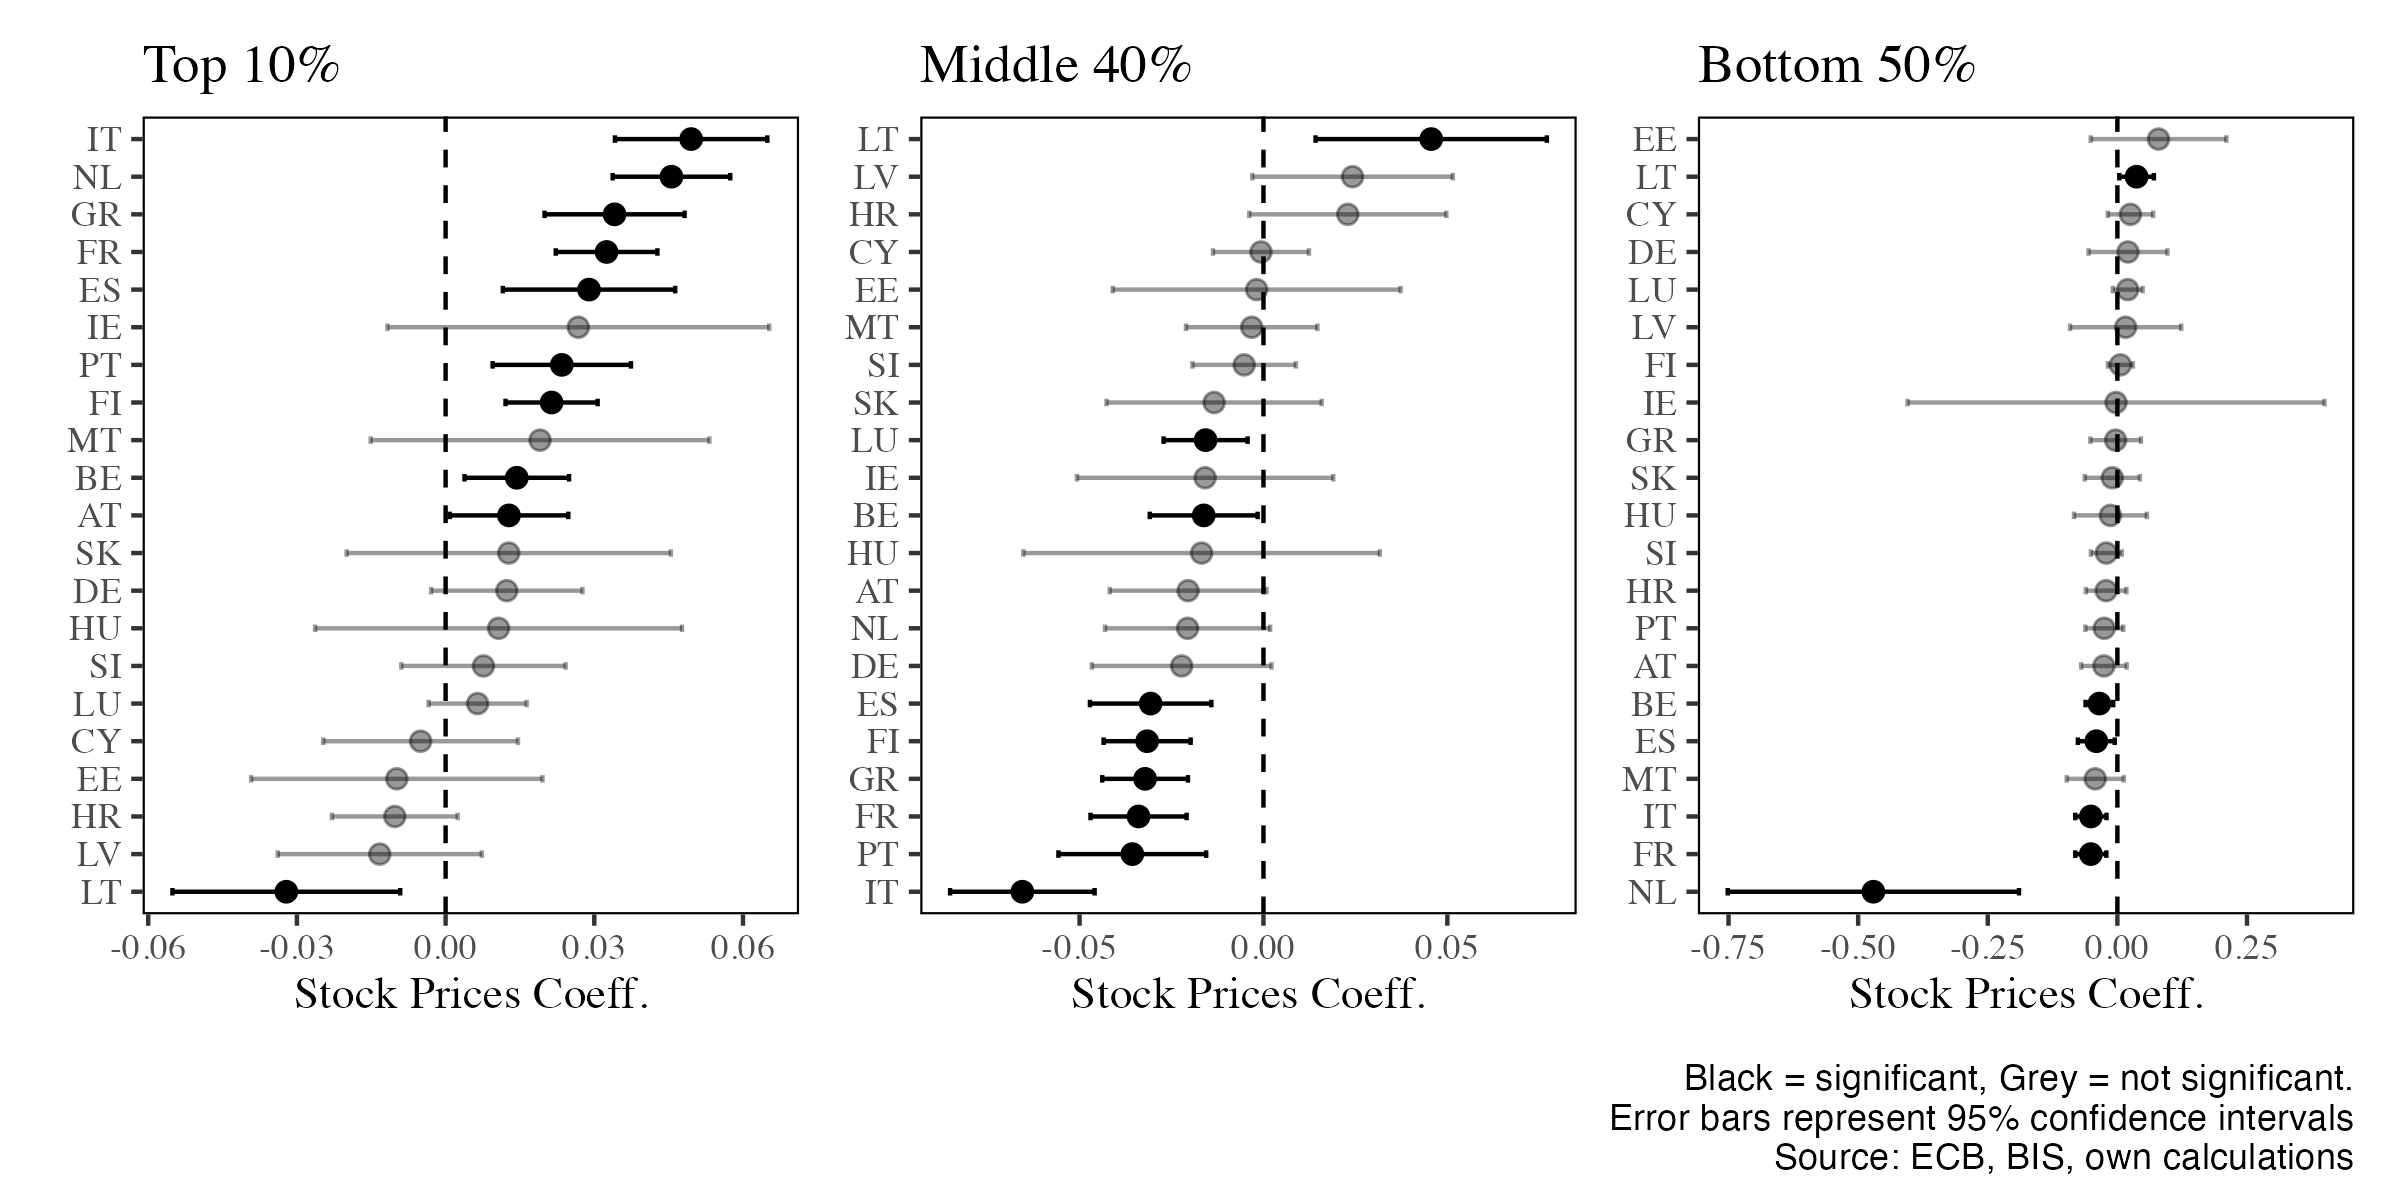
\includegraphics[keepaspectratio]{../output/ts_tables/SP_coeff.png}}

}

\caption{\label{fig-coeffStock}Stock Prices Coefficient Plot}

\end{figure}%

\subsection*{Appendix G: Reverse
Causality}\label{appendix-g-reverse-causality}
\addcontentsline{toc}{subsection}{Appendix G: Reverse Causality}

\begin{figure}[h]

\centering{

\pandocbounded{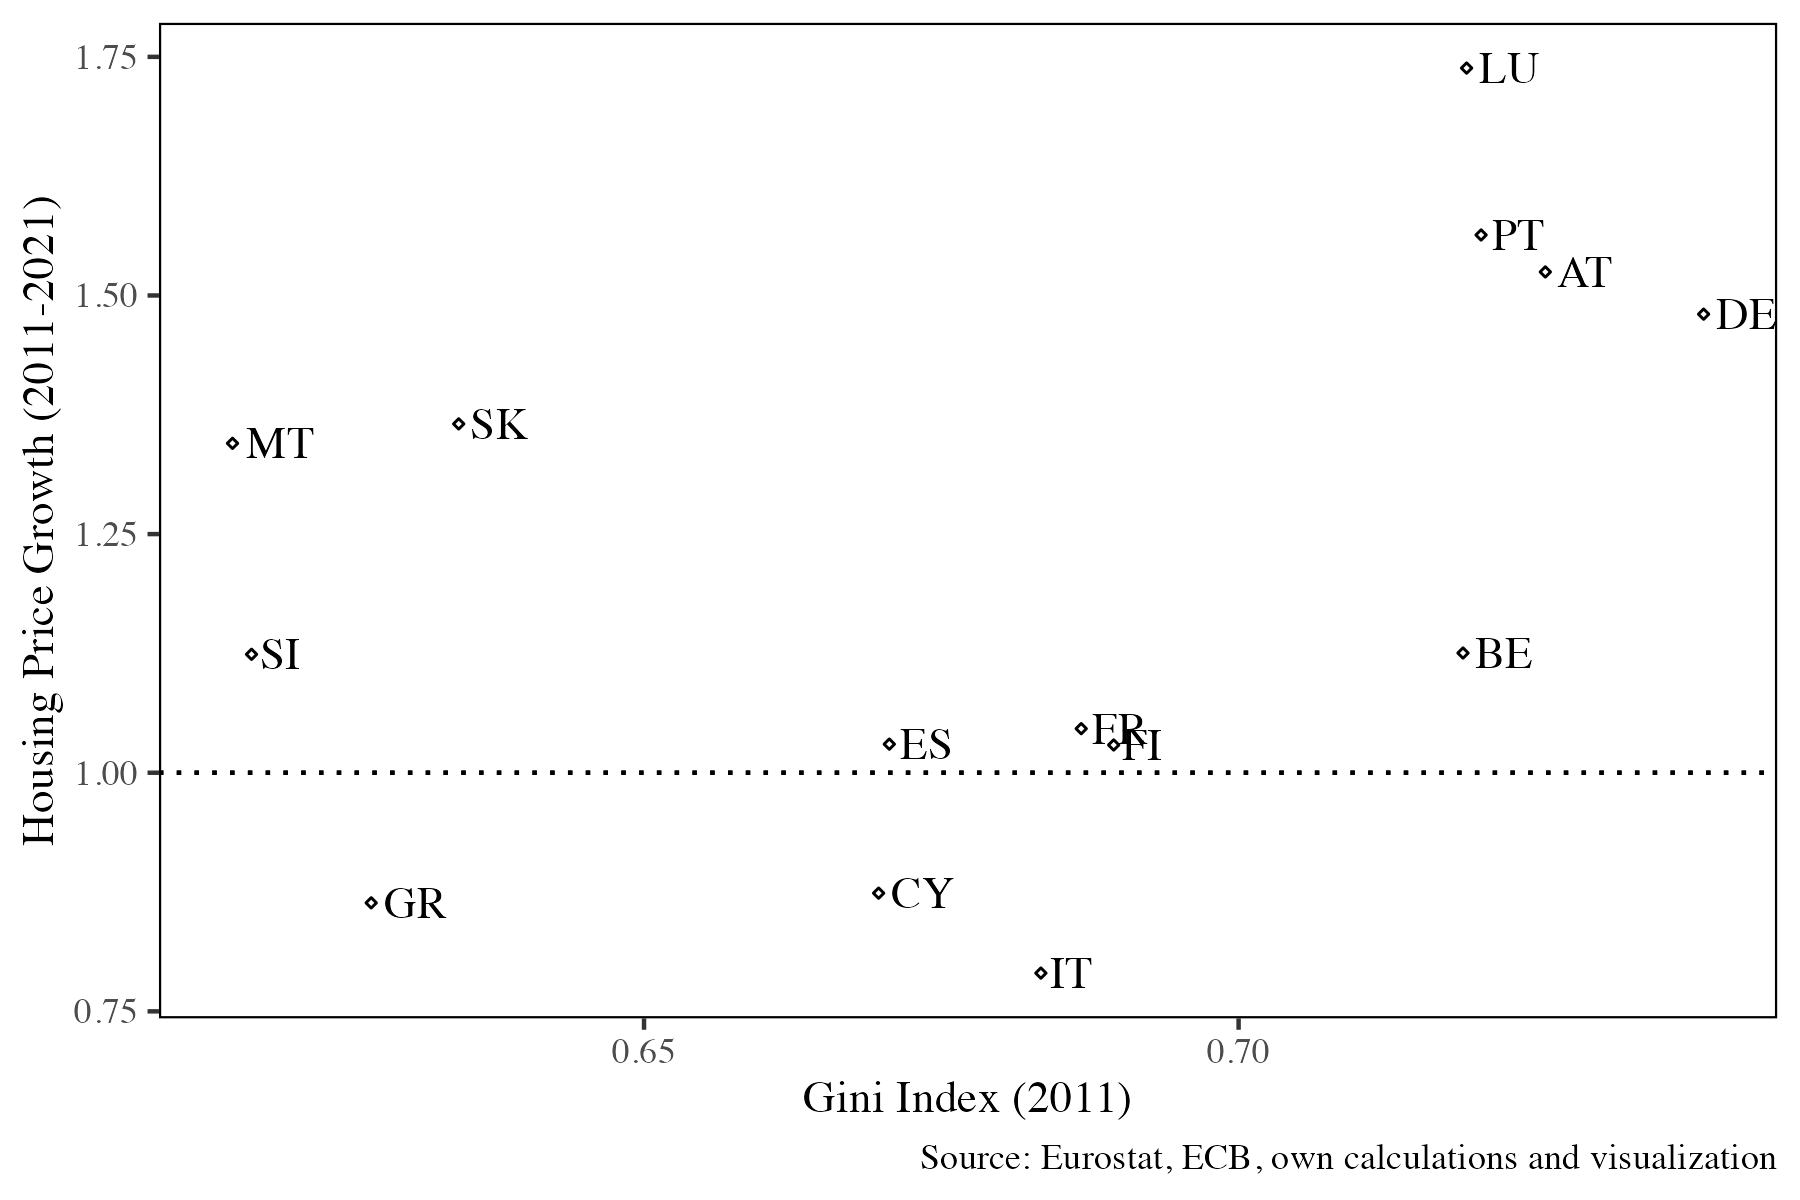
\includegraphics[keepaspectratio]{../output/appendix/hp-ineq.png}}

}

\caption{\label{fig-reverse}Inequality and Housing Price Growth}

\end{figure}%

Figure~\ref{fig-reverse} plots the relationship between the Gini
coefficient at the beginning of a five-year period and the cumulative
growth in real house prices during that period. Two periods are shown:
2014--2019 (red) and 2019--2024 (blue). The year 2014 is used as the
starting point because it maximizes country coverage in the ECB DWA
dataset. The periods are split to account for potential structural
breaks around the COVID-19 pandemic and related policy interventions.
Each point represents a country, and linear fits are shown separately
for each period. The absence of a clear or consistent slope in either
period suggests that higher initial inequality does not robustly predict
stronger house price growth.

\newpage{}

\subsection*{Appendix E: Data and Code}\label{appendix-e-data-and-code}
\addcontentsline{toc}{subsection}{Appendix E: Data and Code}

Data and code used in this thesis are available for reproduction online
at \url{https://github.com/skriptum/inequality}

\newpage{}

\section*{References}\label{references}
\addcontentsline{toc}{section}{References}

\phantomsection\label{refs}
\begin{CSLReferences}{1}{0}
\bibitem[\citeproctext]{ref-adamDistributionalConsequencesAsset2016}
Adam, Klaus, and Panagiota Tzamourani. 2016. {``Distributional
Consequences of Asset Price Inflation in the {Euro Area}.''}
\emph{European Economic Review} 89 (October): 172--92.
\url{https://doi.org/10.1016/j.euroecorev.2016.07.005}.

\bibitem[\citeproctext]{ref-allegreDoesHousingWealth2015}
Allègre, Guillaume, and Xavier Timbeau. 2015. {``{Does housing wealth
contribute to wealth inequality?:A reply to Bonnet et al. (2014)}.''}
\emph{Revue de l'OFCE} 137 (1): 83--95.

\bibitem[\citeproctext]{ref-alvaredoGlobalInequalityDynamics2017}
Alvaredo, Facundo, Lucas Chancel, Thomas Piketty, Emmanuel Saez, and
Gabriel Zucman. 2017. {``Global {Inequality Dynamics}: {New Findings}
from {WID}.world.''} \emph{American Economic Review} 107 (5): 404--9.
\url{https://doi.org/10.1257/aer.p20171095}.

\bibitem[\citeproctext]{ref-bachRichPickingsRisk2020}
Bach, Laurent, Laurent E. Calvet, and Paolo Sodini. 2020. {``Rich
{Pickings}? {Risk}, {Return}, and {Skill} in {Household Wealth}.''}
\emph{American Economic Review} 110 (9): 2703--47.
\url{https://doi.org/10.1257/aer.20170666}.

\bibitem[\citeproctext]{ref-battistiniNavigatingHousingChannel2025}
Battistini, Niccolò, Matteo Falagiarda, Angelina Hackmann, and Moreno
Roma. 2025. {``Navigating the Housing Channel of Monetary Policy Across
Euro Area Regions.''} \emph{European Economic Review} 171 (January):
104897. \url{https://doi.org/10.1016/j.euroecorev.2024.104897}.

\bibitem[\citeproctext]{ref-battyDistributionalFinancialAccounts2022}
Batty, Michael, Jesse Bricker, Joseph Briggs, Sarah Friedman, Danielle
Nemschoff, Eric Nielsen, Kamila Sommer, and Alice Henriques Volz. 2022.
{``The {Distributional Financial Accounts} of the {United States}.''} In
\emph{Measuring {Distribution} and {Mobility} of {Income} and {Wealth}},
641--78. University of Chicago Press.

\bibitem[\citeproctext]{ref-bernankeWhatExplainsStock2005}
Bernanke, Ben S., and Kenneth N. Kuttner. 2005. {``What {Explains} the
{Stock Market}'s {Reaction} to {Federal Reserve Policy}?''} \emph{The
Journal of Finance} 60 (3): 1221--57.
\url{https://doi.org/10.1111/j.1540-6261.2005.00760.x}.

\bibitem[\citeproctext]{ref-bernothECBAssetPurchases2016}
Bernoth, Kerstin, Philipp König, and Benjamin Beckers. 2016. {``{ECB}
Asset Purchases May Affect Wealth Distribution.''} \emph{DIW Economic
Bulletin} 6 (7): 75--81.

\bibitem[\citeproctext]{ref-biewenShapeWealthDistribution2025}
Biewen, Martin, Stefan Glaisner, and Rolf Kleimann. 2025. {``The Shape
of the Wealth Distribution and Differences in Wealth Inequality Across
{Euro} Area Countries.''} \emph{The Journal of Economic Inequality} 23
(1): 1--25. \url{https://doi.org/10.1007/s10888-024-09630-z}.

\bibitem[\citeproctext]{ref-blanchetHowUnequalEurope2019}
Blanchet, Thomas, Lucas Chancel, and Amory Gethin. 2019. {``How {Unequal
Is Europe}? {Evidence} from {Distributional National Accounts},
1980--2017.''} \emph{WID Working Papers}, no. 2019/06 (June).

\bibitem[\citeproctext]{ref-blatnikIntroducingDistributionalWealth2024}
Blatnik, Nina, Alina Bobasu, Georgi Krustev, and Mika Tujula. 2024.
{``Introducing the {Distributional Wealth Accounts} for Euro Area
Households.''} \emph{Economic Bulletin Articles} 5.

\bibitem[\citeproctext]{ref-boelhouwerHousingMarketNetherlands2020}
Boelhouwer, Peter. 2020. {``The Housing Market in {The Netherlands} as a
Driver for Social Inequalities: Proposals for Reform.''}
\emph{International Journal of Housing Policy} 20 (3): 447--56.
\url{https://doi.org/10.1080/19491247.2019.1663056}.

\bibitem[\citeproctext]{ref-bonnetRisingInequalitiesAccess2019}
Bonnet, Carole, Bertrand Garbinti, and Sebastien Grobon. 2019. {``Rising
{Inequalities} in {Access} to {Home Ownership} Among {Young Households}
in {France}, 1973-2013.''} \emph{Banque de France Working Paper}, no.
711 (March). \url{https://doi.org/10.2139/ssrn.3352361}.

\bibitem[\citeproctext]{ref-bonnetDoesHousingCapital2014}
Bonnet, Odran, Pierre-Henri Bono, Guillaume Flamerie de La Chapelle, and
Etienne Wasmer. 2014. {``Does Housing Capital Contribute to Inequality?
{A} Comment on {Thomas Piketty}'s {Capital} in the 21st {Century}.''}

\bibitem[\citeproctext]{ref-bourassaDeterminantsHomeownershipRate2015}
Bourassa, Steven C., Donald R. Haurin, Patric H. Hendershott, and Martin
Hoesli. 2015. {``Determinants of the {Homeownership Rate}: {An
International Perspective}.''} \emph{Journal of Housing Research} 24
(2): 193--210. \url{https://doi.org/10.1080/10835547.2015.12092104}.

\bibitem[\citeproctext]{ref-brechmannRiskManagementHighdimensional2013}
Brechmann, Eike Christain, and Claudia Czado. 2013. {``Risk Management
with High-Dimensional Vine Copulas: {An} Analysis of the {Euro Stoxx}
50.''} \emph{Statistics \& Risk Modeling} 30 (4): 307--42.
\url{https://doi.org/10.1524/strm.2013.2002}.

\bibitem[\citeproctext]{ref-causaHousingWealthAccumulation2019}
Causa, Orsetta, Nicolas Woloszko, and David Leite. 2019. {``Housing,
Wealth Accumulation and Wealth Distribution: {Evidence} and Stylized
Facts.''} \emph{OECD Economics Department Working Papers}, no. 1588
(December).

\bibitem[\citeproctext]{ref-cesa-bianchiHousingCyclesMacroeconomic2013}
Cesa-Bianchi, Ambrogio. 2013. {``Housing Cycles and Macroeconomic
Fluctuations: {A} Global Perspective.''} \emph{Journal of International
Money and Finance} 37 (October): 215--38.
\url{https://doi.org/10.1016/j.jimonfin.2013.06.004}.

\bibitem[\citeproctext]{ref-choTaxTreatmentOwner2011}
Cho, Sang-Wook (Stanley), and Johanna L. Francis. 2011. {``Tax Treatment
of Owner Occupied Housing and Wealth Inequality.''} \emph{Journal of
Macroeconomics}, {SI}: {Macroeconomics} with {Frictions}, 33 (1):
42--60. \url{https://doi.org/10.1016/j.jmacro.2010.09.002}.

\bibitem[\citeproctext]{ref-coakleyUnobservedHeterogeneityPanel2006}
Coakley, Jerry, Ana-María Fuertes, and Ron Smith. 2006. {``Unobserved
Heterogeneity in Panel Time Series Models.''} \emph{Computational
Statistics \& Data Analysis}, Statistical signal extraction and
filtering, 50 (9): 2361--80.
\url{https://doi.org/10.1016/j.csda.2004.12.015}.

\bibitem[\citeproctext]{ref-coccoPortfolioChoicePresence2005}
Cocco, João F. 2005. {``Portfolio {Choice} in the {Presence} of
{Housing}.''} \emph{The Review of Financial Studies} 18 (2): 535--67.
\url{https://doi.org/10.1093/rfs/hhi006}.

\bibitem[\citeproctext]{ref-coenMonetaryShocksHouse2024}
Coën, Alain, and Alexis Pourcelot. 2024. {``Monetary Shocks and House
Prices in {Europe}.''} \emph{Journal of European Real Estate Research}
17 (3): 331--72. \url{https://doi.org/10.1108/JERER-12-2023-0050}.

\bibitem[\citeproctext]{ref-croissantPlmLinearModels2023}
Croissant, Yves, Giovanni Millo, Kevin Tappe, Ott Toomet, Christian
Kleiber, Achim Zeileis, Arne Henningsen, Liviu Andronic, and Nina
Schoenfelder. 2023. {``Plm: {Linear Models} for {Panel Data}.''}

\bibitem[\citeproctext]{ref-driscollConsistentCovarianceMatrix1998}
Driscoll, John C., and Aart C. Kraay. 1998. {``Consistent {Covariance
Matrix Estimation} with {Spatially Dependent Panel Data}.''} \emph{The
Review of Economics and Statistics} 80 (4): 549--60.
\url{https://doi.org/10.1162/003465398557825}.

\bibitem[\citeproctext]{ref-ducaWhatDrivesHouse2021}
Duca, John V., John Muellbauer, and Anthony Murphy. 2021. {``What
{Drives House Price Cycles}? {International Experience} and {Policy
Issues}.''} \emph{Journal of Economic Literature} 59 (3): 773--864.
\url{https://doi.org/10.1257/jel.20201325}.

\bibitem[\citeproctext]{ref-engelDevelopingReconciledQuarterly2022}
Engel, Janina, Pau Gayà Riera, Joseph Grilli, and Pierre Sola. 2022.
{``Developing Reconciled Quarterly Distributional National Wealth:
{Insight} into Inequality and Wealth Structures.''} \emph{ECB Working
Paper}, no. 2687 (July). \url{https://doi.org/10.2866/412495}.

\bibitem[\citeproctext]{ref-eurostatGiniCoefficientEquivalised2024}
EUROSTAT. 2024. {``Gini Coefficient of Equivalised Disposable Income by
Age.''} \url{https://doi.org/10.2908/ILC_DI12}.

\bibitem[\citeproctext]{ref-fagerengHeterogeneityPersistenceReturns2020}
Fagereng, Andreas, Luigi Guiso, Davide Malacrino, and Luigi Pistaferri.
2020. {``Heterogeneity and {Persistence} in {Returns} to {Wealth}.''}
\emph{Econometrica} 88 (1): 115--70.
\url{https://doi.org/10.3982/ECTA14835}.

\bibitem[\citeproctext]{ref-fratzscherECBUnconventionalMonetary2016}
Fratzscher, Marcel, Marco Lo Duca, and Roland Straub. 2016. {``{ECB
Unconventional Monetary Policy}: {Market Impact} and {International
Spillovers}.''} \emph{IMF Economic Review} 64 (1): 36--74.
\url{https://doi.org/10.1057/imfer.2016.5}.

\bibitem[\citeproctext]{ref-fullerHousingPricesWealth2020}
Fuller, Gregory W., Johnston, and Aidan and Regan. 2020. {``Housing
Prices and Wealth Inequality in {Western Europe}.''} \emph{West European
Politics} 43 (2): 297--320.
\url{https://doi.org/10.1080/01402382.2018.1561054}.

\bibitem[\citeproctext]{ref-godaAbsoluteIncomeInequality2020}
Goda, Thomas, Chris Stewart, and Alejandro Torres García. 2020.
{``Absolute Income Inequality and Rising House Prices.''}
\emph{Socio-Economic Review} 18 (4): 941--76.
\url{https://doi.org/10.1093/ser/mwz028}.

\bibitem[\citeproctext]{ref-hickHousingAffordabilityPoverty2024}
Hick, Rod, Marco Pomati, and Mark Stephens. 2024. {``Housing
Affordability and Poverty in {Europe}: On the Deteriorating Position of
Market Renters.''} \emph{Journal of Social Policy}, January, 1--24.
\url{https://doi.org/10.1017/S0047279423000703}.

\bibitem[\citeproctext]{ref-hsiaoBayesEstimationShortrun1999}
Hsiao, Cheng, M. Hashem Pesaran, and A. Kamil Tahmiscioglu. 1999.
{``Bayes Estimation of Short-Run Coefficients in Dynamic Panel Data
Models.''} In \emph{Analysis of {Panels} and {Limited Dependent Variable
Models}}, edited by Cheng Hsiao, M. Hashem Pesaran, Kajal Lahiri, and
Lung Fei Lee, 1st ed., 268--96. Cambridge University Press.
\url{https://doi.org/10.1017/CBO9780511493140.013}.

\bibitem[\citeproctext]{ref-jordaGreatMortgagingHousing2016}
Jordà, Òscar, Moritz Schularick, and Alan M. Taylor. 2016. {``The Great
Mortgaging: Housing Finance, Crises and Business Cycles.''}
\emph{Economic Policy} 31 (85): 107--52.
\url{https://doi.org/10.1093/epolic/eiv017}.

\bibitem[\citeproctext]{ref-kaasWealthInequalityHomeownership2019}
Kaas, Leo, Georgi Kocharkov, and Edgar Preugschat. 2019. {``Wealth
{Inequality} and {Homeownership} in {Europe}.''} \emph{Annals of
Economics and Statistics}, no. 136: 27--54.
\url{https://doi.org/10.15609/annaeconstat2009.136.0027}.

\bibitem[\citeproctext]{ref-kaasLowHomeownershipGermany2021}
Kaas, Leo, Georgi Kocharkov, Edgar Preugschat, and Nawid Siassi. 2021.
{``Low {Homeownership} in {Germany}---a {Quantitative Exploration}.''}
\emph{Journal of the European Economic Association} 19 (1): 128--64.
\url{https://doi.org/10.1093/jeea/jvaa004}.

\bibitem[\citeproctext]{ref-kimDynamicStockMarket2005}
Kim, Suk Joong, Fariborz Moshirian, and Eliza Wu. 2005. {``Dynamic Stock
Market Integration Driven by the {European Monetary Union}: {An}
Empirical Analysis.''} \emph{Journal of Banking \& Finance} 29 (10):
2475--2502. \url{https://doi.org/10.1016/j.jbankfin.2004.09.002}.

\bibitem[\citeproctext]{ref-kuhnIncomeWealthInequality2020}
Kuhn, Moritz, Moritz Schularick, and Ulrike I. Steins. 2020. {``Income
and {Wealth Inequality} in {America}, 1949--2016.''} \emph{Journal of
Political Economy} 128 (9): 3469--519.
\url{https://doi.org/10.1086/708815}.

\bibitem[\citeproctext]{ref-martinez-toledanoHousePriceCycles2022}
Martínez-Toledano, Clara. 2022. {``House {Price Cycles}, {Wealth
Inequality} and {Portfolio Reshuffling},''} World {Inequality Database
WORKING PAPER},.

\bibitem[\citeproctext]{ref-mathaHouseholdWealthEuro2017}
Mathä, Thomas Y., Alessandro Porpiglia, and Michael Ziegelmeyer. 2017.
{``Household Wealth in the Euro Area: {The} Importance of
Intergenerational Transfers, Homeownership and House Price Dynamics.''}
\emph{Journal of Housing Economics} 35 (March): 1--12.
\url{https://doi.org/10.1016/j.jhe.2016.12.001}.

\bibitem[\citeproctext]{ref-milloPanelTimeSeries2018}
Millo, Giovanni, and Yves Croissant. 2018. {``Panel {Time Series}.''} In
\emph{Panel {Data Econometrics} with {R}}, 185--209. John Wiley \& Sons,
Ltd. \url{https://doi.org/10.1002/9781119504641.ch8}.

\bibitem[\citeproctext]{ref-nesshoeferRanglisteGroesstenVermoegen2024}
Neßhöfer, Christoph, and Andreas Bornefeld. 2024. {``{Rangliste der
gr{ö}{ß}ten Verm{ö}gen 2024}.''} \emph{manager magazin}, October.

\bibitem[\citeproctext]{ref-networkEurosystemHouseholdFinance2013}
Network, Eurosystem Household Finance and Consumption. 2013. {``The
{Eurosystem Household Finance} and {Consumption Survey} - {Results} from
the First Wave.''} Working \{\{Paper\}\} 2. ECB Statistics Paper.
\url{https://doi.org/10.2866/12862}.

\bibitem[\citeproctext]{ref-neweyHypothesisTestingEfficient1987}
Newey, Whitney K., and Kenneth D. West. 1987. {``Hypothesis {Testing}
with {Efficient Method} of {Moments Estimation}.''} \emph{International
Economic Review} 28 (3): 777--87. \url{https://doi.org/10.2307/2526578}.

\bibitem[\citeproctext]{ref-pesaranTimeSeriesPanel2015}
Pesaran, M. Hashem. 2015. \emph{Time {Series} and {Panel Data
Econometrics}}. Oxford University Press.

\bibitem[\citeproctext]{ref-pesaranEstimatingLongrunRelationships1995}
Pesaran, M. Hashem, and Ron Smith. 1995. {``Estimating Long-Run
Relationships from Dynamic Heterogeneous Panels.''} \emph{Journal of
Econometrics} 68 (1): 79--113.
\url{https://doi.org/10.1016/0304-4076(94)01644-F}.

\bibitem[\citeproctext]{ref-pikettyCapitalTwentyFirstCentury2014}
Piketty, Thomas. 2014. \emph{Capital in the {Twenty-First Century}}.
Harvard University Press. \url{https://doi.org/10.4159/9780674369542}.

\bibitem[\citeproctext]{ref-pikettyIncomeInequalityUnited2003}
Piketty, Thomas, and Emmanuel Saez. 2003. {``Income {Inequality} in the
{United States}, 1913--1998*.''} \emph{The Quarterly Journal of
Economics} 118 (1): 1--41.
\url{https://doi.org/10.1162/00335530360535135}.

\bibitem[\citeproctext]{ref-pikettyDistributionalNationalAccounts2018}
Piketty, Thomas, Emmanuel Saez, and Gabriel Zucman. 2018.
{``Distributional {National Accounts}: {Methods} and {Estimates} for the
{United States}*.''} \emph{The Quarterly Journal of Economics} 133 (2):
553--609. \url{https://doi.org/10.1093/qje/qjx043}.

\bibitem[\citeproctext]{ref-pikettyCapitalBackWealthIncome2014a}
Piketty, Thomas, and Gabriel Zucman. 2014. {``Capital Is {Back}:
{Wealth-Income Ratios} in {Rich Countries} 1700--2010 *.''} \emph{The
Quarterly Journal of Economics} 129 (3): 1255--1310.
\url{https://doi.org/10.1093/qje/qju018}.

\bibitem[\citeproctext]{ref-runstlerBusinessHousingCredit2018}
Rünstler, Gerhard, and Marente Vlekke. 2018. {``Business, Housing, and
Credit Cycles.''} \emph{Journal of Applied Econometrics} 33 (2):
212--26. \url{https://doi.org/10.1002/jae.2604}.

\bibitem[\citeproctext]{ref-savvaStockMarketIntegration2010}
Savva, Christos S., and Nektarios Aslanidis. 2010. {``Stock Market
Integration Between New {EU} Member States and the {Euro-zone}.''}
\emph{Empirical Economics} 39 (2): 337--51.
\url{https://doi.org/10.1007/s00181-009-0306-6}.

\bibitem[\citeproctext]{ref-scatignaResidentialPropertyPrice2014}
Scatigna, Michela, Robert Szemere, and Kostas Tsatsaronis. 2014.
{``Residential {Property Price Statistics Across} the {Globe}.''}
\{\{SSRN Scholarly Paper\}\}. Rochester, NY: Social Science Research
Network.

\bibitem[\citeproctext]{ref-sierminskaOwnNotOwn2013}
Sierminska, Eva, and Karina Doorley. 2013. {``To Own or Not to Own?
{Household} Portfolios, Demographics and Institutions in a
Cross-National Perspective.''} Working \{\{Paper\}\} 611. SOEPpapers on
Multidisciplinary Panel Data Research.

\bibitem[\citeproctext]{ref-stephensPikettyInequalityHousing2017}
Stephens, Mark. 2017. {``Piketty, {Inequality} and {Housing}.''}
\emph{Housing, Theory and Society} 34 (2): 167--70.
\url{https://doi.org/10.1080/14036096.2017.1293381}.

\bibitem[\citeproctext]{ref-vermeulenEstimatingTopTail2016}
Vermeulen, Philip. 2016. {``Estimating the {Top Tail} of the {Wealth
Distribution}.''} \emph{American Economic Review} 106 (5): 646--50.
\url{https://doi.org/10.1257/aer.p20161021}.

\bibitem[\citeproctext]{ref-wolffTopHeavyStudy1995}
Wolff, Edward N. 1995. \emph{Top Heavy: A Study of the Increasing
Inequality of Wealth in {America}}. A {Twentieth Century Fund} Report.
Twentieth Century Fund Press.

\bibitem[\citeproctext]{ref-wolffHeterogenousRatesReturn2025}
---------. 2025. {``Heterogenous {Rates} of {Return} on {Homes}: {Do The
Rich Do Better}?''} \emph{Review of Income and Wealth} 71 (1): e12704.
\url{https://doi.org/10.1111/roiw.12704}.

\bibitem[\citeproctext]{ref-wooldridgeIntroductoryEconometricsModern2013}
Wooldridge, Jeffrey M. 2013. \emph{Introductory {Econometrics}: {A
Modern Approach}}. Cengage Learning.

\end{CSLReferences}

\newpage{}




\end{document}
